%% An Introduction to LaTeX Thesis Template of Wuhan University
%%
%% Created by WHUTUG

% !TeX program = xelatex

\documentclass[type=master, class=academic]{whu-thesis}
\usepackage{rotating}
\renewcommand{\cleardoublepage}{\clearpage}
% 注释掉下面这行编译出来的即为插入空白页，不注释则为不插入空白页
% 针对前几页有效

\newcommand{\figcite}[1]{\scalebox{1.3}[1.3]{\raisebox{-0.7ex}{\cite{#1}}}}
\whusetup
  {
    info               =
      {
        title          = {分布式信源编码辅助的\\编码计算结果传输方法研究},
        title*         = {Revisiting Distributed Source Coding for Expedited Downlink Transmission in Coded Edge Computing},
%%%%% ------------------------------------------------------------------- %%%%%
        student-number = {2023202120067},
        school         = {电子信息学院},
        school*        = {Electronic Information School},
        author         = {胡蓉},
        author*        = {\sc Hu~Rong},
        clc            = {},%%%%%
        % subject        = {学科},
        major          = {信息与通信工程},
        major*         = {Information and Communication Engineering},
        advisor        = {贺晓帆, 教授},
        advisor*       = {\sc Prof.~He~Xiaofan},
        direction      = {编码边缘计算},%%%%
        direction*     = {Coded Edge Computing},%%%%
        date           = {2026/5},
        keywords       = {编码边缘计算, 分布式信源编码, 伴随式穿刺, 嵌套线性码, 非正交多址接入},
        keywords*      = {Coded Edge Computing; Distributed Source Coding; Syndrome Puncturing; Nested Linear Codes; Non-Orthogonal Multiple Access},
      },
    style              =
    {
    	graphics-path  = {{figures/}{data/}},
    	list-of-figures,
    	list-of-tables,
    	% bib-backend    = {bibtex},
    	bib-style      = {numerical},
    	cite-style     = {numerical-super},
    	cjk-font       = overleaf
    },
    element            =
      {
        innovation     = {pages/innovation},
        abstract       = {pages/abstract},
        abstract*      = {pages/enabstract},
        bibliography   = {refs},
        appendix       = {pages/appendix},
        achievements   = {pages/achievements},
        thanks         = {pages/thanks}
      }
  }

\usepackage{amsfonts}
\usepackage{bbm}
\usepackage{pifont}
\usepackage{setspace}
\usepackage{cases}
\usepackage{bm}
\usepackage{multirow}
\usepackage{arydshln}
%\usepackage[subrefformat=parens]{subfig}
\newcommand{\upcite}[1]{{\setcitestyle{square,super}\cite{#1}}}
% \allowdisplaybreaks[4]
\usepackage{xurl}
\begin{document}

\renewcommand{\cleardoublepage}{\clearpage}

%%----------- 主体部分 ----------- %%
% Chapter 1

\chapter{绪论}

\section{研究背景与意义}
近年来，无线通信与物联网技术的持续演进在一定程度上推动了社会信息化的进程，使得移动终端规模与数据流量呈现出稳步增长的趋势。根据中华人民共和国工业和信息化部发布的《2025年通信业统计公报》，截至2025年底，我国移动电话用户总数达到18.27亿户，全年移动互联网接入流量累计为3958亿GB，全国移动电话基站总数也已扩充至1287万个\upcite{miit2025}。
这些基础设施的建设与数据规模的增长，为虚拟现实\upcite{7946930}、增强现实\upcite{8329628}、自动驾驶\upcite{liu2021vehicular}等应用场景的落地提供了基本的网络环境。与此同时，此类新兴应用对计算能力和响应时延提出了更为具体的挑战。以自动驾驶辅助系统为例，其在运行过程中需要对周围环境数据进行及时的分析与处理，以协助完成安全决策。在远程医疗或工业协作场景中，网络延迟的波动往往会直接影响到任务的执行效率。然而，随着应用需求的日益多样化，在处理上述新兴业务时，传统的计算模式逐渐暴露出一些客观存在的局限性。首先，受限于便携式终端设备的物理尺寸与电池容量，其本地运算能力往往难以独立支撑复杂的计算任务。其次，
传统的云计算模式通过将计算任务传输至远端云服务器处进行处理并返回计算结果\upcite{8016573,patel2014mobile}。在应对高频率、低时延的任务处理时，这种计算模式将受限于长距离传输和中心化处理，暴露出资源分布不均或响应滞后等实际问题，难以满足某些对实时性要求较高的应用场景。

\begin{figure}[htbp]
	\centering
	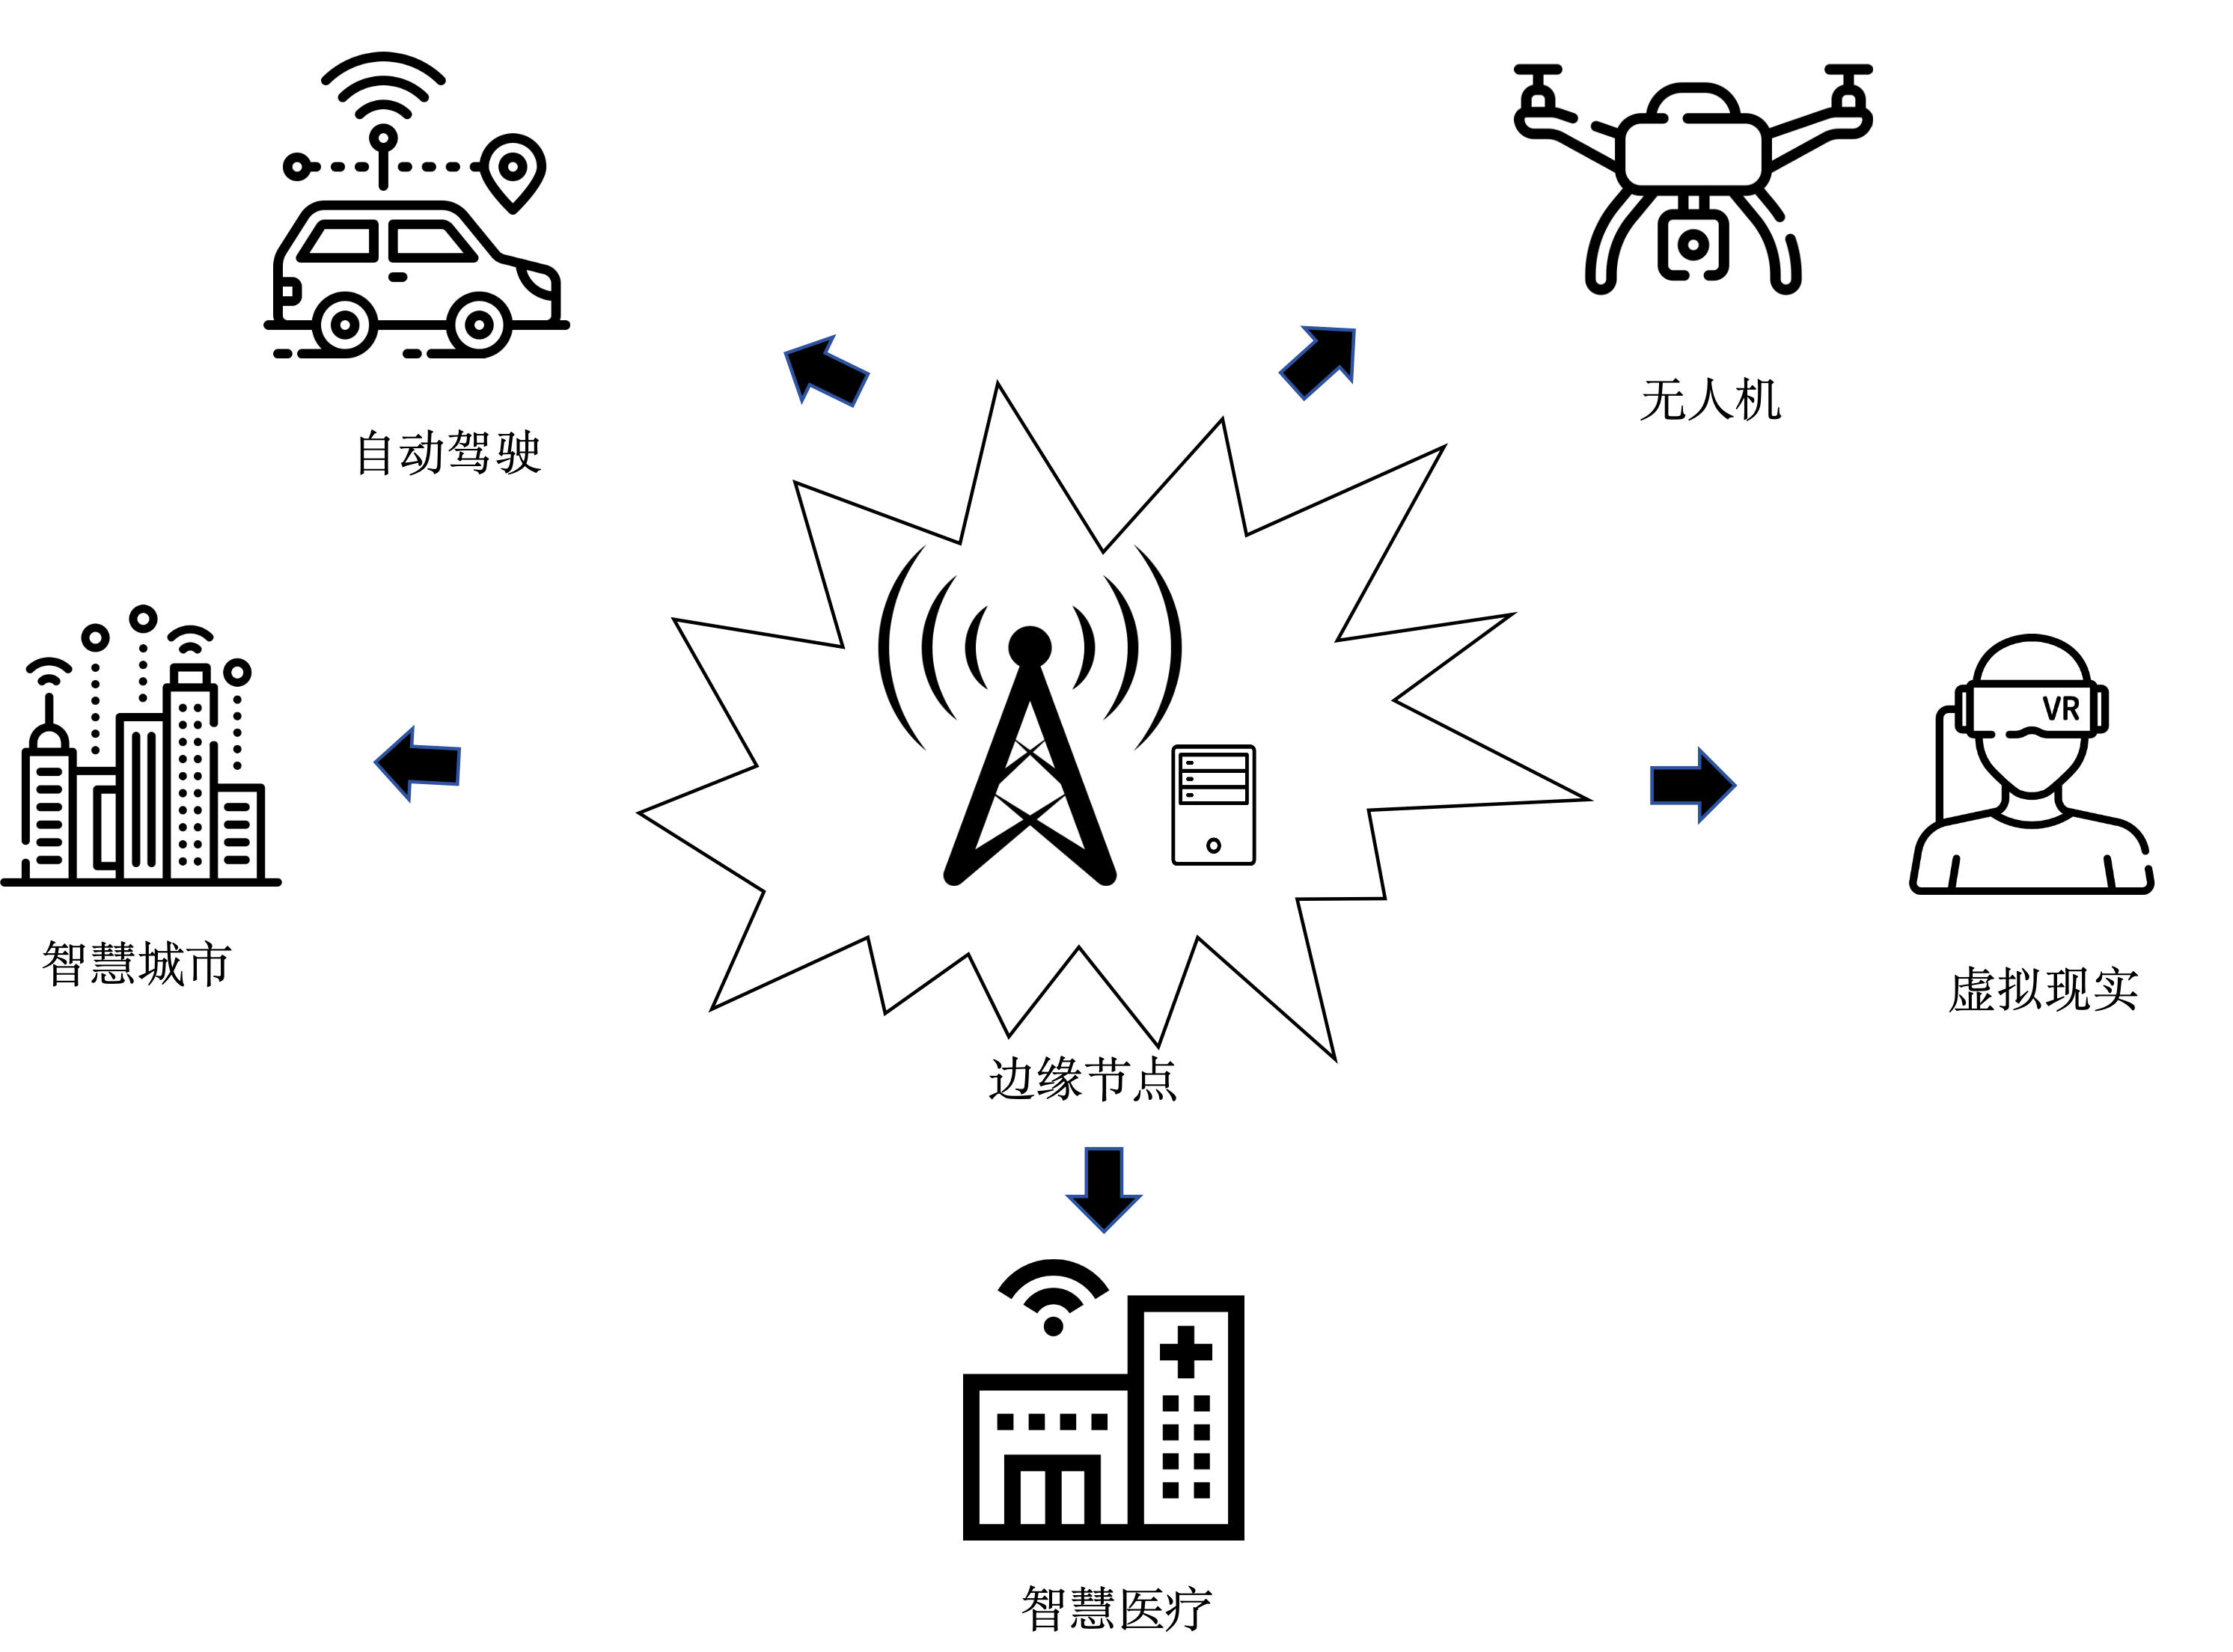
\includegraphics[width=0.6\textwidth]{figures/边缘计算示例图.png}
	\caption{边缘计算应用场景示意图}
	\label{fig-Edge-Computing-Application}
\end{figure}

针对这些实际需求，边缘计算作为一种新兴计算范式，受到了学术界与工业界的关注\upcite{8016573,patel2014mobile}。早在2014年，欧洲电信标准协会（European Telecommunications Standards Institute）正式提出了边缘计算的概念\upcite{patel2014mobile}。其核心思想是通过在网络边缘部署计算资源，使得移动设备可以将算力需求较高的任务卸载至网络边缘的节点上进行计算并回传计算结果，从而起到降低响应时延、缓解终端能耗压力的作用。目前，边缘计算已成为5G及未来移动通信网络中的关键技术方向之一，并在虚拟/增强现实\upcite{9363323,9789210}、自动驾驶\upcite{10213996,8584062}、无人机\upcite{9778241,uavassited}、智慧城市\upcite{10551400,9063670}、智慧医疗\upcite{10339657,11008531}等诸多领域获得了广泛应用。

然而，随着应用数据的持续激增以及计算任务的规模持续扩大（如智能驾驶\upcite{autodriving}，人工智能\upcite{10333824,10835069}等），单一节点的计算资源难以进一步支持大规模的计算任务并满足低时延的需求。因此，集中式的边缘计算架构将向分布式边缘计算架构演进\upcite{gong2020delay,7796149,9827607}。分布式边缘计算通过聚合网络边缘多个节点的计算资源，将原始的大规模任务分解为多个规模较小的子任务，并将其分发至网络中的多个边缘节点并行执行，从而提升计算效率和计算延迟。
尽管分布式边缘计算在处理大规模计算任务方面具有显著优势，但其性能上限往往受限于迟滞效应\upcite{ng2021comprehensive,7848828}。具体来说，在实际的边缘网络环境中，由于边缘节点的硬件配置、负载状态以及网络环境存在异构性，部分节点可能会因资源竞争或突发故障等随机因素导致其计算速度远远落后于其他节点，这类节点将成为迟滞节点。由于分布式边缘计算往往需要等待所有子任务的返回结果才能恢复最终计算结果，整体计算时间往往取决于计算最慢的边缘节点。因此，迟滞边缘节点的存在将严重增加总体时延，甚至会削弱分布式边缘计算带来的优势。

为了缓解分布式边缘计算中的迟滞效应，编码计算作为一种具备容错能力的计算范式，为提升计算效率和可靠性提供了新的研究思路\upcite{ng2021comprehensive,9155226,8002642}。受经典纠错码理论的启发\upcite{lin2004error}，编码边缘计算通过在计算任务分发阶段引入冗余，即将原始任务划分为多个子任务，利用编码技术将这些子任务编码成一组具有冗余特性的编码子任务，并将其部署至各边缘节点并行处理。得益于编码子任务之间的冗余特性，中心节点或移动终端不再需要等待所有边缘节点均完成计算，而仅需要收到部分执行较快节点的计算结果，即可通过解码操作重构出完整的原始计算任务结果。这种以冗余换取计算延迟的方案缓解了由个别边缘节点计算滞后带来的时延问题，从而在一定程度上优化了分布式系统的运行效率\upcite{2021-10-2187}。

尽管编码计算在缓解迟滞效应方面有显著的效果\upcite{peng2020diversity}，但大多数研究往往忽视了无线通信阶段带来的挑战\upcite{8002642}。在实际的编码计算应用中，无线信道条件往往也会对系统性能产生制约。部分处于深度衰落或遭受严重干扰的边缘节点，其较差的信道条件会导致严重的通信延迟，进而导致整体计算任务的完成时长，削弱编码计算在应对迟滞效应时带来的效益。为了缓解通信延迟带来的影响，目前针对编码计算传输机制的研究，通常将边缘节点的下行传输视为传统的多用户通信问题，即假设各节点发送的消息是相互独立的\upcite{9046826,9829189,9328810,9820783}，忽略了由于引入编码理论而存在的子任务间冗余信息特性。事实上，由于编码边缘计算在任务分发阶段采用了编码技术，不同边缘节点计算出的中间结果之间存在着强相关性。如果能充分挖掘并利用这部分冗余信息，将为优化无线传输带来新的可能性。

基于此，研究发现编码计算可以类比于经典的分布式信源编码（Distributed Source Coding, DSC）技术，即多个分布式信源与一个接收方共同通信\upcite{1055037,1328091}。在经典信息论中，分布式信源编码理论指出，对于相关联的分布式信源，即使节点间不进行通信，也可以通过联合解码实现更高效的数据压缩。然而，现有的编码计算相关工作尚未充分挖掘与经典分布式信源编码理论结合带来的通信优化潜力。因此，通过引入分布式信源压缩编码理论，提出能加速下行传输的优化编码计算结果传输机制具有重要的研究意义。

\section{国内外研究现状}
由于编码计算通过引入冗余信息有效缓解了分布式边缘计算中存在的迟滞效应，近年来大多工作开始聚焦于编码计算。但由于大多数工作只关注了计算延迟，忽略了下行传输可能造成的通信延迟。因此，本文主要针对利用DSC辅助的编码计算下行传输方法展开研究。本节将分别从编码计算以及分布式信源编码两方面对国内外研究现状进行介绍。


\subsection{编码计算}

近年来，编码边缘计算在缓解迟滞效应方面展现出显著优势，其核心思想是融合纠删码理论与分布式边缘计算。具体来说，编码计算将原始计算任务划分为多个子任务，并通过灵活多样的编码方法转化为多个编码子任务，中心节点将这些编码子任务分发给边缘节点进行并行计算，仅需要接收到部分执行较快的边缘节点的计算结果即可恢复原始计算任务的结果。该思想目前已经广泛应用于大规模矩阵乘法、分布式梯度下降以及多项式函数计算等任务中。 在矩阵乘法中，文献\cite{8002642}和文献\cite{8006963}中首次提出了利用最大距离可分（Maximum Distance Separable， MDS）码对原始矩阵进行分块编码的方案，确保中心节点仅需收集到任意恢复阈值个边缘节点的计算结果即可重构原始任务的计算结果。该方法显著的降低了整体的任务处理延迟。然而，随着计算规模的扩大，单一维度的编码往往面临恢复阈值过高的局限。针对大规模矩阵-矩阵乘法，文献\cite{720548}引入了乘积码（Product code），通过在行与列两个维度同时实施编码，实现了更高的编码效率。 文献\cite{yu2017polynomial}提出了多项式码（Polynomial code），通过为每个边缘节点分配不同的随机数，并使用该随机数对输入矩阵进行编码，使得解码过程可采用多项式插值方式。该方案通过将子任务的构造与重构过程映射至多项式空间，成功实现了恢复阈值与边缘节点数量的解耦，可以实现最优恢复阈值，且该恢复阈值不随着边缘节点数量的变化而变化。基于多项式码，文献\cite{dutta2019optimal}提出MatDot码，通过增加通信成本，进一步降低了恢复阈值。由于MatDot码的通信成本较高，该文献进一步在MatDot基础上提出了PolyDot权衡了恢复阈值和通信成本之间的关系。此外，文献\cite{yu2020straggler}在多项式码的基础上提出了纠缠多项式码（Entangled polynomial code），允许对输入矩阵进行任意划分，而不是只能按列划分。纠缠多项式码能够进一步利用系统资源，保证在相同恢复阈值的情况下，降低边缘节点的工作负载。

在分布式学习场景中，编码计算也有广泛的应用。文献\cite{tandon2017gradient}中首次提出了梯度编码，通过将编码后的训练数据和计算任务存储在边缘节点，使得中心节点能够容忍部分迟滞节点。具体来说，梯度编码通过将训练数据集分为多个批次，由主节点将部分数据批分配给边缘节点，边缘节点进行数据集的训练得到部分梯度值，并根据编码系数将梯度值的线性组合返回给主节点，主节点可以根据任意恢复阈值个边缘节点的梯度值利用解码系数恢复全梯度。文献\cite{halbawi2018improving}进一步利用里德-所罗门（Reed-Solomon）码构造了一种梯度编码方式，保证了工作负载相同的情况下能够进一步降低恢复阈值。文献\cite{cao2021adaptive}提出了一种自适应梯度编码方案，更适用于迟滞节点数量未知的情况。具体来说，该方案中边缘节点在完成梯度计算后向中心节点发送信号，如果中心节点可以直接恢复全梯度则边缘节点将不需要继续返回编码梯度，如果存在迟滞节点，则边缘节点将继续返回编码梯度，直到主节点恢复全梯度。针对多项式函数计算等非线性计算任务场景，文献\cite{yu2019lagrange}提出了拉格朗日编码方案，通过利用拉格朗日插值多项式对计算任务进行编码，解码时只需重构多项式即可恢复原始计算任务的结果。文献\cite{jahani2022berrut}进一步提出近似多项式插值编码方案，实现了恢复误差和恢复阈值间的平衡。针对矩阵乘法中矩阵具有稀疏性的场景，文献\cite{10633712}提出了一种保持矩阵稀疏性的编码方法，以降低迟滞节点的影响。

在上述编码机制的基础上，许多工作进一步研究了编码计算中的参数选择以及计算任务分配等。例如，文献\cite{8002642}中将计算延迟建模为服从指数分布的随机变量，通过优化MDS码的编码参数来最小化计算时延。针对特定计算任务（如分布式矩阵乘法）。文献\cite{peng2020diversity}中分别建模了三种不同分布的计算时延模型，并分析了不同模型下编码参数的选择对计算时延的影响。此外，文献\cite{8663353}研究了异构集群场景，通过在预算约束下优化边缘节点之间的负载分配来加速计算。文献\cite{9641837}则提出了一种部分恢复方案，通过牺牲计算精度来换取更快的响应速度，实现了精度与延迟之间的平衡。

然而，编码边缘计算的端到端时延不仅取决于计算延迟，还取决于无线通信过程带来的传输延迟。当边缘节点处于深衰落或拥塞信道时，通信延迟往往成为系统瓶颈。为此，近年来的研究开始转向计算与通信的联合优化 \upcite{9820783,9606237,9046826,9829189}。例如，文献\cite{9606237}提出了一种基于块划分（block-division）的方案，利用迟滞节点的局部计算结果，通过适当调整子块的数量来平衡计算与通信之间的延迟。文献\cite{9820783}设计了一种基于块设计的无线Luby-Transform（LT）码的传输方案，有效实现了二者的良好折中。此外，文献\cite{7935426,8051074}开发了一种可扩展的编码计算框架，通过巧妙地创造高效的多播机会来降低通信开销。文献\cite{9046826}利用负载分配策略联合优化计算和通信延迟。文献\cite{9829189}针对一般性的衰落信道环境，提出了一种延迟最优的编码卸载方案，同时优化编码参数和边缘节点的选择策略，以降低总延迟。
上述研究大多只考虑边缘节点独立传输其计算结果，未充分挖掘编码任务间由于相关性可能带来的协作潜力。为此，部分研究开始探索编码边缘计算中的协作传输机制，旨在利用编码冗余提升传输效率。例如，文献\cite{9328810}设计了一种基于MDS码和重复码级联的任务卸载策略，利用更多的非掉队节点进行协作传输。类似的协作形式也在文献\cite{8691770,9062599}中进行了探讨。文献\cite{9562193}则将LT码与不规则重复码相结合，以产生空间分集增益，从而实现编码边缘计算中的协作下行传输。

尽管上述工作在节点间协作传输上进行了研究，但大多将编码计算的传输过程视为传统的多用户通信问题，主要依赖增加空间分集或简单的重复传输来提升可靠性。然而，编码计算的本质在于任务编码引入了数据冗余，导致不同节点的计算结果之间存在强相关性。现有方案未能利用分布式信源编码挖掘这一相关性带来的压缩增益，这为进一步降低通信延迟留下了更多的优化空间。


\subsection{分布式信源编码}
分布式信源编码是一种旨在解决多个相互关联但独立编码但信源压缩问题的技术范式\upcite{1055037,1328091,1055508,cover1999elements,Tberger}。其核心思想是即使各信源节点在编码节点无法进行信息交互，只要解码端掌握了信源间的统计相关性，系统仍然可以以接近联合编码的比特率实现信息的有效传输。在早期的文献\cite{1055037}中，SW定理利用随机分箱方法对无损恢复的压缩极限给出了理论的分析，文献\cite{cover1999elements}进一步将SW理论的可行性推广到了任意遍历过程以及任意数量的相关信源场景。文献\cite{1055508}中也给出了相似的联合高斯信源的有损压缩极限理论分析。此后，分布式信源编码理论已被广泛应用于多个领域\upcite{1328091,1542403,761254,10620735}。例如，文献\cite{761254}利用分布式信源编码刻画了卫星通信的可行压缩率区域并加速传输。文献\cite{10620735}在边缘网络自动驾驶场景中研究了信源信道联合优化。文献\cite{4567562, 4313115}则深入探讨了分布式信源编码系统的鲁棒性、安全性以及存在窃听者时的编码问题。具体来说，文献\cite{4567562}开发了一种能够平衡系统鲁棒性和压缩效率的DSC方案，文献\cite{4313115}研究了存在窃听者情况下的DSC问题。

在这些应用的推动下，DSC技术成为了研究热点。
然而SW定理只给出了理论极限，如何设计实际的编码方案实现这个理论区域一直是研究难题\cite{1328091}。早期的工作主要考虑非对称编码方案，即通过实现SW理论区域的角点达到压缩极限，例如，文献\cite{1184140}和文献\cite{,1512420}采用基于伴随式的方法来实现SW区域的角点。随后，文献\cite{1281475}中提出了能够逼近SW区域边界任意点的编码方案。随着信道编码技术的发展，文献\cite{1055171}最先注意到了DSC与信道编码之间的紧密联系，并提出使用线性信道码作为SW编码的一种构造方法，并在文献\cite{1184140}中被用于基于信道码（如卷积码）的实际SW编码设计。此后，这种将信源编码映射到互不相交的信道码陪集中的方案可以被扩展到所有二进制具有线性关系的信源场景。为了逼近SW极限，许多工作将低密度奇偶校验码（Low-Density Parity-Check,  LDPC）和Turbo码\upcite{910571}应用在分布式信源编码中并扩展至多信源、非二进制以及信源存在记忆相关性场景。例如，文献 \cite{1281525}提出了基于LDPC码的分布式信源编码方案以实现多进制信源的角点压缩。文献\cite{1413577}则利用Turbo码将非二进制符合转换为比特序列进行压缩。文献\cite{1187376}则考虑了信源间存在记忆相关性，利用LDPC码压缩存在记忆相关性的信源，所得性能接近理论SW极限。对于一般的非二进制多信源场景，设计能够覆盖整个SW区域的实用码字仍具挑战性。文献 \cite{1281474}提出的L-machine方法和文献 \cite{1661834}提出的信源分裂方法虽然在理论上可行，但在实际实现中往往面临计算复杂度过高的问题。此外，部分研究关注特定的相关模型（如线性关系），其通用性比较受限 \cite{1614079,6241374} 。近期，文献\cite{10557705}尝试利用基于机器学习的方法构建分布式编码器和解码器，但目前主要局限于有损压缩的场景。然而，实际应用通常需要处理连续信源编码，即如何保证失真度的情况下，对分布式信源进行压缩编码问题。文献\cite{1055508}对SW定理的两个信源非对称编码方案推广到带有边信息的单端有损压缩场景，即结合量化技术对离散信源的编码实现相对于保真度准则而非无损压缩，并给出了该问题的速率-失真函数，被称为Wyner-Ziv极限。文献\cite{1197848}则进一步将文献\cite{1055508}中给出的速率-失真函数从高斯分布推广到了更任意的分布。由于SW定理的实际编码方案是基于信道编码的，对于有损连续信源的实际编码本质上是一个信源-信道联合编码问题，其中包含了由信源编码引起的量化损失以及信道编码引起的噪声损失。为了逼近Wyner-Ziv极限，文献\cite{1003821}引入嵌套格码（Nested lattice codes）可以在高维信源下渐进地达到Wyner-Ziv极限，并且实际的嵌套格码最早由文献\cite{838191}实现。对于多信源分布式有损压缩场景，文献\cite{tung1978multiterminal}和文献\cite{1056105}进一步提出了对连续信源进行量化后再编码方案所能达到的速率范围，称为Berger-Tung可达区域。

上述工作大多都致力于恢复独立信源，然而在一些场景（如分布式机器学习）中，解码端只需要得到所有信源的线性组合。经典SW区域和Berter-Tung区域虽然在独立恢复信源方面效果较好，但在恢复特定相关性信源或者分布式函数计算时，可能不是最优的，即存在信息冗余，从而导致传输效率较低。基于此，一些工作针对线性恢复信源的场景展开了研究\cite{1056022,1057272,4797745,6481622}。对于两个信源恢复线性组合时，文献\cite{1057272}对线性计算函数进行了分类，当线性计算函数等效于独立恢复信源时，可达压缩区域与SW区域完全重合，即需要传输足够恢复原始信源的全部信息。当线性计算函数为可进一步压缩的函数时，存在一些信源分布，使得恢复信源线性组合时所需的可达速率小于SW区域，意味着这种情况下利用函数的结构可以进行更高效的压缩编码。例如，文献\cite{1056022}中给出了经典Körner-Marton 问题（计算两个二进制信源的模二和）的可达速率区域，该区域的最小可达速率严格小于SW编码所需的速率。文献\cite{4797745}提出使用嵌套阿尔贝群码（Nested Abelian group codes）将复杂的多端信源编码问题分解为多个数位上的编码问题，利用代数结构实现了比Berger-Tung更小的可达速率区域。针对多信源的线性函数计算，文章\cite{6481622}提出了基于嵌套线性码的编码方案，并在一些特殊情况下证明了比SW区域更优的压缩区域。文章\cite{lim2019towards}进一步证明了使用嵌套线性码联合典型性解码的信源编码可达速率区域。尽管上述研究给出了信源编码压缩的极限区域，针对完整恢复多信源的场景，现有的分布式信源编码研究大多侧重于特殊的相关模型或仅关注理论极限，缺乏具有普适性的编码方案。在编码边缘计算场景中，计算结果之间存在由代数编码引入的线性相关结构，目前尚缺乏利用这一特性设计的高效、实用的分布式信源编码方法。针对线性函数恢复场景，现有的相关研究尚未与编码边缘计算场景结合，缺乏对两者的实际应用研究。

综上所述，尽管编码边缘计算的相关研究在计算延迟和简单的传输优化方面已取得显著进展，但针对其下行传输的协作传输方面仍需要投入更多的研究。现有的通信方案主要基于独立传输或简单的协作分集，忽视了计算结果间的强相关性。通过引入分布式信源编码，可以充分的利用这部分强相关性。然而，分布式信源编码理论已经比较成熟，但针对编码计算这一特定场景的实用化设计仍然缺失。因此，探索编码边缘计算传输与经典的分布式信源编码问题之间的关系，并利用计算相关性进行高效信源编码的传输方案，具有重要的学术价值和应用前景。

\section{主要研究内容与论文结构}

结合当前国内外的研究现状，现有编码计算的无线传输过程仍面临一些问题。首先，现有大多数研究只考虑编码计算的计算延迟，忽略了下行传输过程中由于信道衰落可能导致的通信延迟。其次，编码计算中通过任务编码使得子任务间具有相关性，现有多数研究并未充分利用这部分相关性，并认识到其与DSC问题的联系。
针对编码边缘计算中由于任务编码引入的信息冗余特性，本研究将从分布式信源编码的视角出发，深入研究面向完整重构计算结果和线性恢复计算结果两种场景下，编码计算结果传输机制与分布式信源编码的联合优化，进一步提升编码计算中下行传输的性能，主要研究内容可归纳为以下两个方面：
\begin{enumerate}[label=(\arabic*)]
	\item {面向独立恢复的DSC辅助编码计算结果传输方法研究。}
	针对编码计算中需要完整重构计算结果的场景，如何有效缓解计算较快的节点信道条件差导致的传输延迟是本研究需要考虑的问题。为此，本研究考虑将分布式信源编码与编码计算结合，提出一种DSC辅助的编码计算结果传输机制。具体来说，
	本研究利用编码计算结果之间存在的强相关性，结合经典SW定理，刻画在无通信条件下实现计算结果完整恢复的理论压缩区域，深入分析由MDS码等线性任务编码方案在边缘节点计算结果中引入的数学相关性，建立编码计算下行传输的速率区域模型。此外，经典SW定理的压缩区域往往难以实现，为了实现SW定理的子区域，本研究设计一种基于LDPC码的分布式信源编码方案。提出基于伴随式穿刺的编码方案，使边缘节点能够根据信道状态自适应地调整截断或扩展伴随式长度。依据上述思路，本研究建立了基于数据完整恢复的传输时延最小化模型，通过设计优化算法联合优化各边缘节点的信源压缩率与传输功率，达到节点间基于信道状态的负载重分配效果，并通过实验仿真验证性能。
	\item {面向线性恢复的DSC辅助编码计算结果传输方法研究。}
	针对仅需获取计算结果线性和值的场景，由于不需要完整恢复计算结果，如何进一步压缩信源达到比完整恢复更大的压缩区域是本研究考虑的问题。本研究发现利用嵌套线性码进行信源编码可以证明在只需要恢复计算结果线性和值时，可以达到比完整重构更高的压缩效率。具体来说，通过引入嵌套线性码构造策略，利用数据的线性结构特性，允许边缘节点对数据进行特殊的线性编码，使得中心节点利用同时联合典型性解码技术，直接从接收到的叠加信号中解码出目标函数。依据上述思路，本研究设计基于计算感知的传输机制，建立最小化时延模型，并设计相应的优化算法，并通过实验仿真验证性能。
	
\end{enumerate}

\begin{figure}[t]
    \centering
    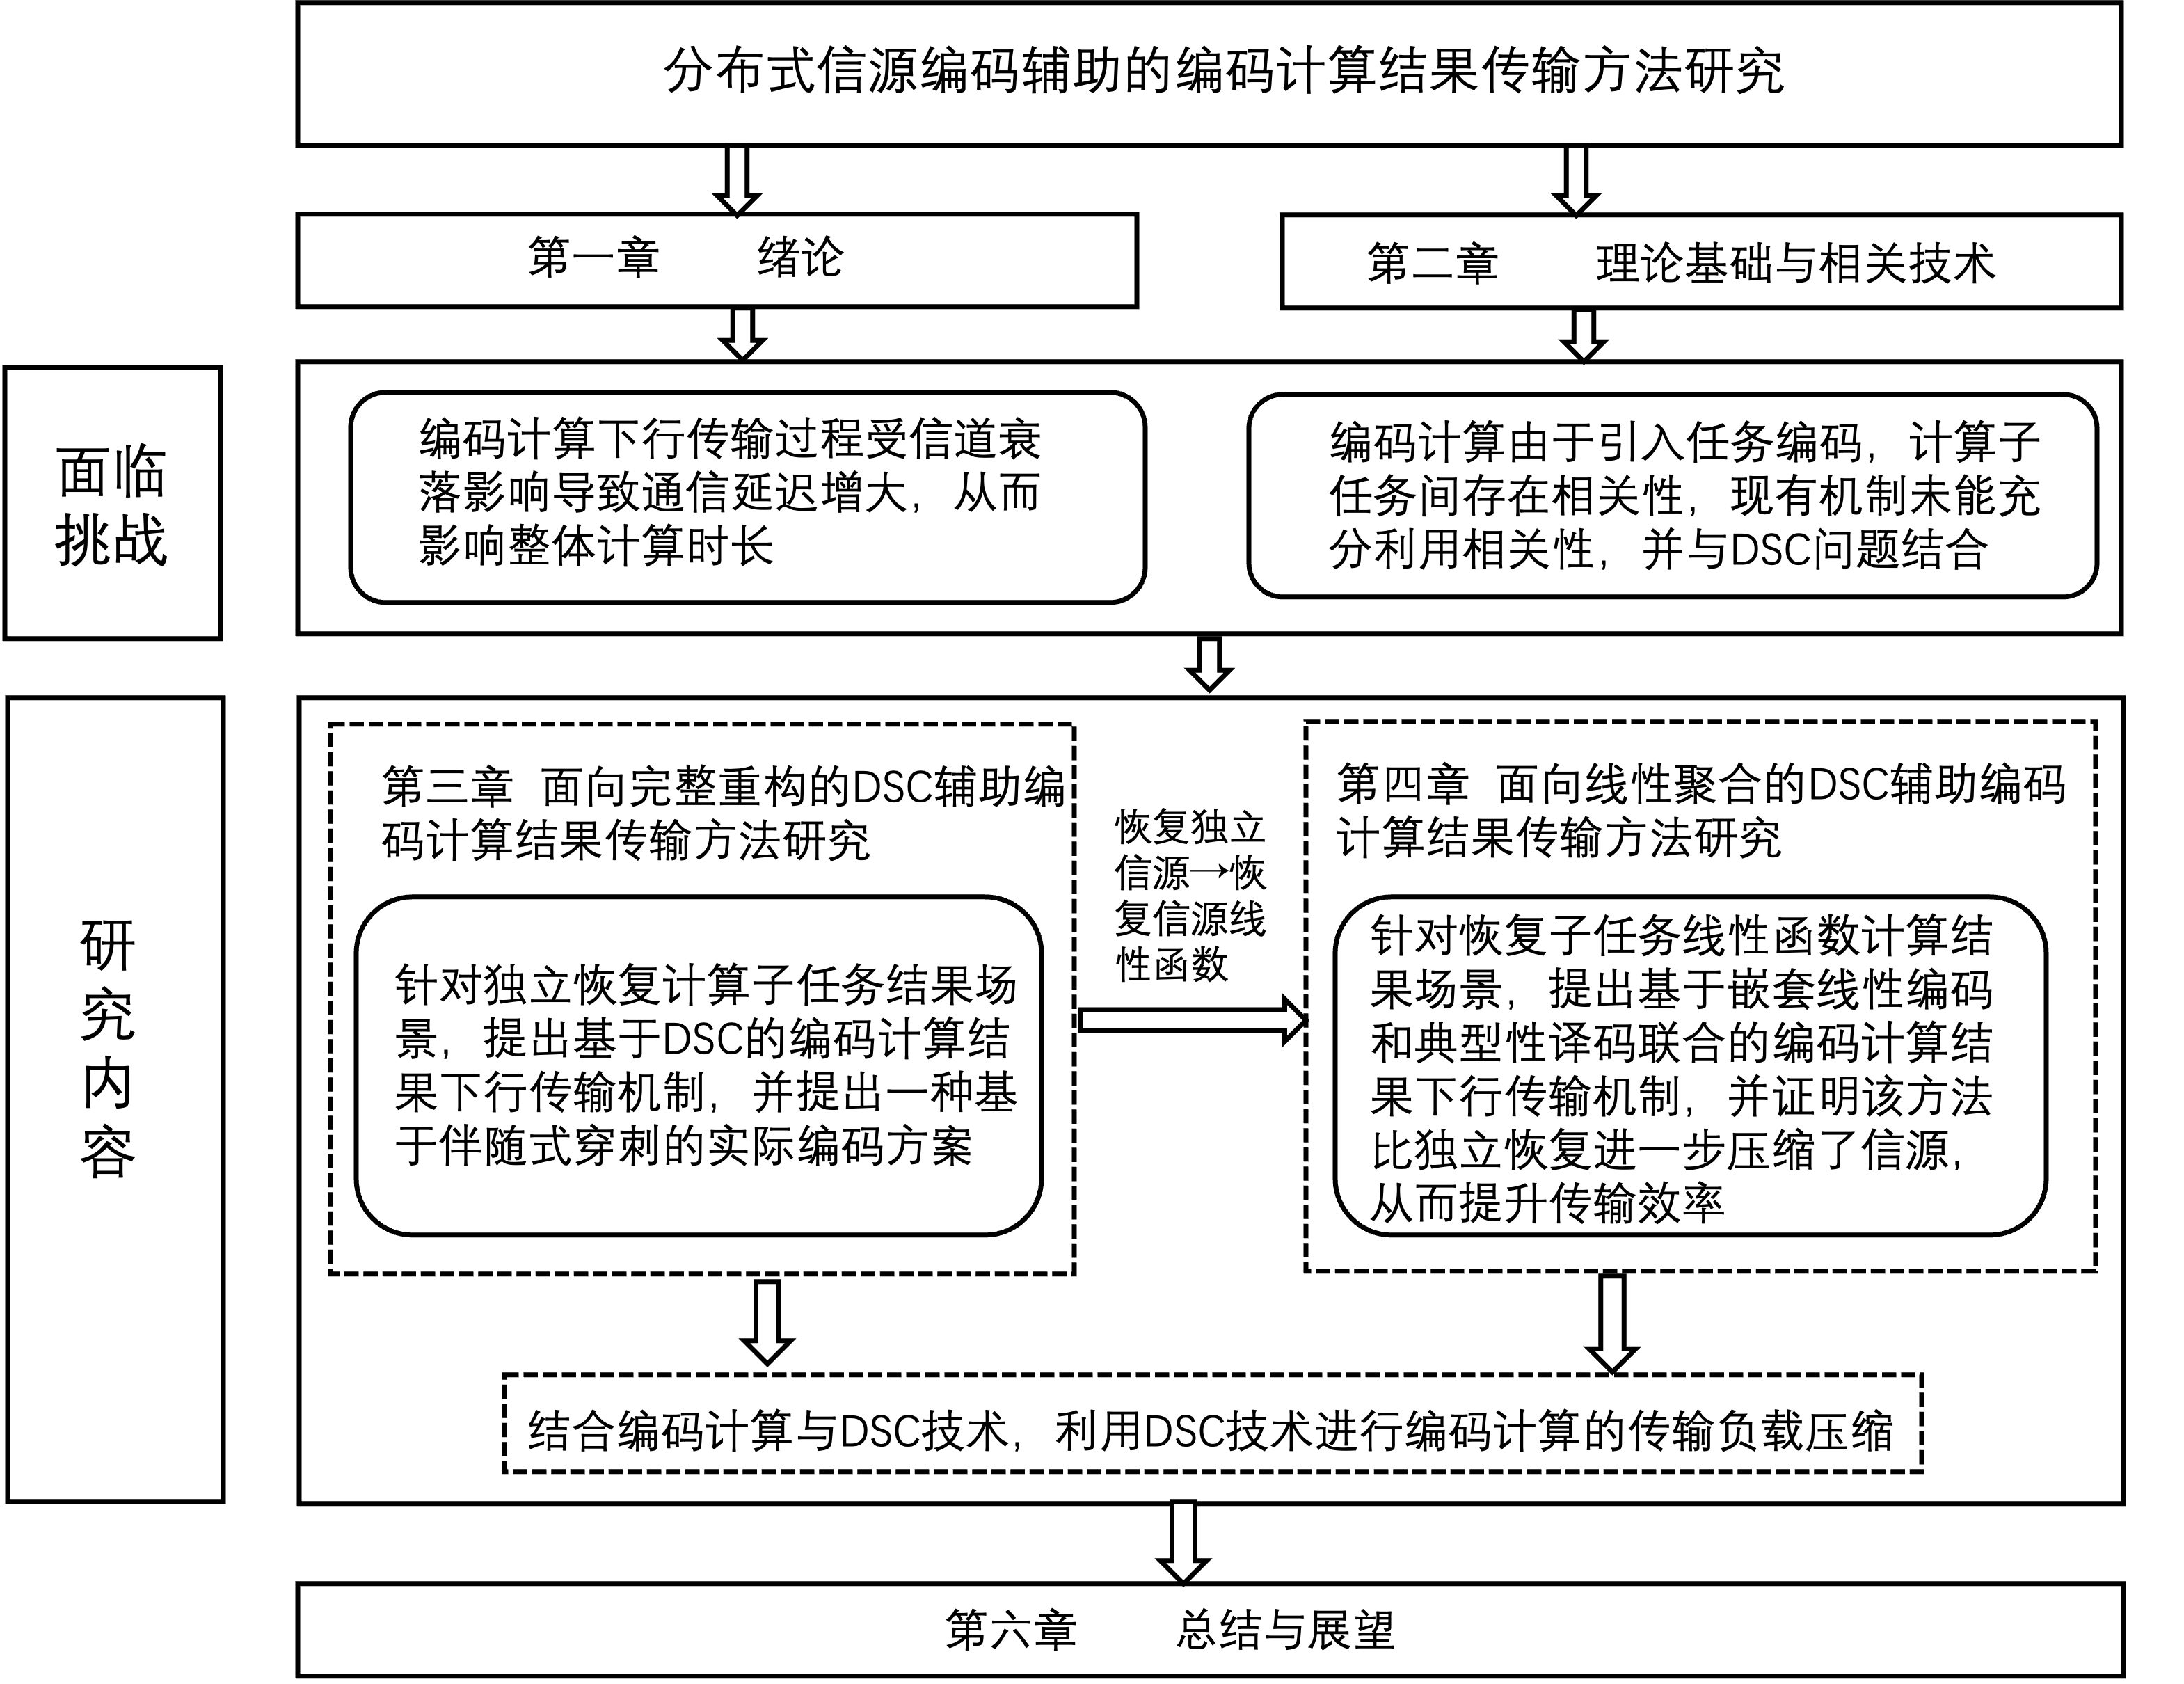
\includegraphics[width=0.97\textwidth]{研究内容与结构.png}
    \caption{本文组织结构与安排}
    \label{figure-origanization}
\end{figure}

根据上述研究内容，本文的各章节联系如\ref{figure-origanization}所示。具体内容安排如下：

第一章，绪论。该章节介绍了分布式信源编码辅助的编码计算结构方法的研究背景与意义，并总结了编码计算方法、编码计算中无线通信机制以及DSC问题的研究现状，分析了现有机制存在的问题。

第二章，理论基础与相关技术。该章节首先介绍了编码计算的基本概念以及梯度编码的编码计算方法以及无损DSC的基本概念以及针对线性函数计算的信源编码方法。随后介绍了编码计算的下行过程传输技术采用的非正交多址技术，以及最优化理论与方法，为本文后续的各研究内容问题建模和求解提供了理论基础。

第三章，面向完整重构的DSC辅助编码计算结果传输方法。针对独立恢复计算子任务结果的场景，该章节提出了基于DSC的编码计算结果下行传输机制。首先，基于理论信源压缩极限，对编码计算下行传输过程进行建模。为了实现信源压缩，之后该章节提出了基于伴随式穿刺的具体DSC方案，并推导出了该方案对应的压缩区域。随后，该章节将所提机制扩展到了高维数据的场景。基于上述机制，本章建模了相应的编码计算最小化下行传输延迟问题，利用凹凸过程对该问题进行求解，在此基础上，本章提出了问题求解的优化算法，并通过数值仿真结果验证了所提机制的有效性。

第四章，面向线性聚合的DSC辅助编码计算结果传输方法研究。针对恢复子任务线性函数计算场景，本章提出了面向线性恢复的DSC辅助编码计算结果下行传输机制。给出了基于嵌套线性码编码和典型性译码下的信源压缩极限，并基于该极限值进行了编码计算下行传输最小化优化问题的建模。随后，提出了具体的优化算法，并通过数值仿真验证所提机制的有效性。

第五章，总结与展望。该章节对本文的研究内容进行了总结，并进一步探讨了DSC应用编码计算的更多研究方向。


\chapter{理论基础与相关技术}

本文主要研究DSC辅助的编码计算结果传输方法，包括面向完整重构子任务的计算结果和面向恢复子任务计算结果的线性函数。因此，本章将对涉及的理论基础和相关技术进行阐述，为后续章节所提传输机制提供理论支撑。首先，本章将介绍编码计算的基本原理，重点阐述MDS码和梯度编码方法。其次，本章将介绍经典无损DSC问题，包括完整恢复的SW定理以及恢复线性函数时使用的嵌套线性码。最后，本章将介绍编码计算下行传输利用的非正交多址技术以及凹凸过程算法等原理。



\section{编码计算}

分布式边缘计算通过将计算任务划分为多个子任务并分发至多个边缘节点并行处理来降低时延。因此，主节点需要等待所有边缘节点完成计算并返回计算结果后才能恢复原始任务的计算结果。然而， 由于边缘节点可能由于系统故障等随机因素造成计算失败，进而拖长整体的计算延迟。编码边缘计算通过引入纠删码理论向计算任务中注入冗余，可以有效缓解迟滞效应带来的影响。具体来说，在编码边缘计算场景中，主节点将原始计算任务划分为多计算子任务，并通过纠删码，生成多个编码子任务，随后将编码子任务分发给边缘节点进行计算，主节点仅需接收到部分节点的计算结果即可恢复原始任务的计算结果，从而避免等待迟滞节点。
为更清晰的展示编码边缘计算的原理，图\ref{coded edge computing}以矩阵-向量乘法为例，展示了下行传输过程，假设移动设备需要计算矩阵乘法任务$\mathbf{X}=\mathbf{A}\mathbf{b}$。利用编码边缘计算的原理，移动设备首先将计算任务按行划分为三个子矩阵$\mathbf{A}_1$、$\mathbf{A}_2$、$\mathbf{A}_3$，并利用(5,3)线性码编码成五个编码子矩阵，分别是$\mathbf{A}_1^{enc}=\mathbf{A}_1$、$\mathbf{A}_2^{enc}=\mathbf{A}_2$、$\mathbf{A}_3^{enc}=\mathbf{A}_3$、$\mathbf{A}_4^{enc}=\mathbf{A}_1+\mathbf{A}_2+\mathbf{A}_3$、$\mathbf{A}_5^{enc}=\mathbf{A}_1+2\mathbf{A}_2+3\mathbf{A}_3$。随后，移动设备将这些编码子任务分发给边缘节点并行处理，当任意三个或更多节点完成计算后，完成计算的边缘节点将它们的计算结果发送给移动设备。假设边缘节点3和边缘节点4由于随机故障成为了迟滞节点，无法完成计算任务。移动设备
在收到节点1、节点2和节点5的计算结果后即可通过$\mathbf{X}_1=\mathbf{Y}_1$、$\mathbf{X}_2=\mathbf{Y}_2$以及$\mathbf{X}_3=(\mathbf{Y}_5-\mathbf{Y}_1-2\mathbf{Y}_2)/3$恢复未编码子任务计算结果，原始计算结果$\mathbf{X}$可以通过$\mathbf{X}_1$、$\mathbf{X}_2$以及$\mathbf{X}_3$得到。

\begin{figure}[t]
	\centering
	\includegraphics[width=0.7\textwidth]{figs/SW.pdf}
	\caption{编码计算示例}
	\label{coded edge computing}
\end{figure}

\subsection{面向矩阵-向量乘法的编码计算}
考虑一个包含$N$个计算节点的分布式计算系统，以矩阵-向量乘法任务$\mathbf{X}=\mathbf{A}\mathbf{b}$为例。中心节点首先将矩阵$\mathbf{A}$按行划分为$N$个子矩阵$\left\{\mathbf{A}_i\right\}_{i=1}^N$，并将这些子矩阵分配至计算节点$[N]=\{1,2,\cdots,N\}$，执行计算子任务$\mathbf{X}_i=\mathbf{A}_i\mathbf{b}$。中心节点需要接收到所有计算节点的计算结果$\left\{\mathbf{X}_i\right\}_{i=1}^N$才能恢复原始计算任务的计算结果$\mathbf{X}$。由于分布式计算可能存在迟滞效应，即边缘节点可能由于随机故障导致计算失败，从而增加整体任务的计算时延。为了缓解迟滞效应，可以采用编码计算方法。以采用MDS码对计算任务进行编码\upcite{8002642}为例，在编码过程中，首先利用$ (N,K)$-MDS码将原始矩阵$\mathbf{A}$按行分为$ K$个子矩阵，即$ \textbf{A}=\begin{bmatrix}
	\textbf{A}_1 \\
	\textbf{A}_2 \\
	\cdots \\
	\textbf{A}_K
\end{bmatrix}$。基于MDS码构造编码矩阵$\mathbf{M}=[m_{n,i}]_{n\in[N],i\in[k]}$，利用构造的编码矩阵对划分后的$K$个子矩阵进行编码，生成$N$个编码子矩阵$\left\{\mathbf{A}_{i}^{enc}\right\}_{i=1}^N$，即
\begin{equation}
	\mathbf{A}_{n=1}^{enc}=\sum_{i=1}^K m_{n,i} \mathbf{A}_i, \quad \forall n\in[N].
\end{equation}
在完成编码后，中心节点将编码后的子矩阵$\left\{\mathbf{A}_i^{enc}\right\}_{i=1}^N$分发给$N$个边缘节点执行矩阵-向量乘法计算
\begin{equation}
	\mathbf{Y}_{n}=\mathbf{A}_n^{enc}\mathbf{b}=\sum_{i=1}^K m_{n,i} \mathbf{A}_i \mathbf{b},\quad \forall n\in[N],
\end{equation}
其中，$\mathbf{Y}_i$为编码子任务$i$的编码计算结果。
此时，中心节点最多可以容忍的迟滞者数量为$S=N-K$。当接收到计算最快的$K$个节点$\left\{\pi(1),\pi(2),\cdots,\pi(K)\right\}$的计算结果$\left\{\mathbf{Y}_{\pi(1)},\mathbf{Y}_{\pi(2)},\cdots,\mathbf{Y}_{\pi(K)}\right\}$，其中计算结果满足
\begin{equation}
	\begin{bmatrix}
	 \mathbf{Y}_{\pi(1)} \\
		 \mathbf{Y}_{\pi(2)}  \\
		\cdots   \\
		 \mathbf{Y}_{\pi(K)} 
	\end{bmatrix}=
	\begin{bmatrix}
		m_{\pi(1),1}& m_{\pi(1),2} &\cdots & m_{\pi(1),K}\\
		 m_{\pi(2),1}& m_{\pi(2),2}&\cdots & m_{\pi(1),K}\\
		\cdots & \cdots &\ddots &\cdots \\
		m_{\pi(K),1}& m_{\pi(K),2}&\cdots & m_{\pi(1),K}\	\\              
	\end{bmatrix}
	\begin{bmatrix}
		\textbf{A}_1 \\
		\textbf{A}_2 \\
		\cdots \\
		\textbf{A}_K
	\end{bmatrix}\mathbf{b}.\label{mds}
\end{equation}
根据MDS的特性，编码矩阵中任意$K$列线性无关。因此，令$\mathbf{M}$表示$[m_{\pi(i),k}]_{i,k\in[k]}$，矩阵$\mathbf{M}$为可逆矩阵。在公式（\ref{mds}）两端同时乘以$\mathbf{M}^{-1}$，则可得到原始任务的计算结果$\mathbf{X}$
\begin{equation}
		\mathbf{M}^{-1}	\begin{bmatrix}
		\mathbf{Y}_{\pi(1)} \\
		\mathbf{Y}_{\pi(2)}  \\
		\cdots   \\
		\mathbf{Y}_{\pi(K)} 
	\end{bmatrix} =	\begin{bmatrix}
	m_{\pi(1),1}& m_{\pi(1),2} &\cdots & m_{\pi(1),K}\\
	m_{\pi(2),1}& m_{\pi(2),2}&\cdots & m_{\pi(1),K}\\
	\cdots & \cdots &\ddots &\cdots \\
	m_{\pi(K),1}& m_{\pi(K),2}&\cdots & m_{\pi(1),K}\	\\              
	\end{bmatrix}^{-1}	\begin{bmatrix}
	m_{\pi(1),1}& m_{\pi(1),2} &\cdots & m_{\pi(1),K}\\
	m_{\pi(2),1}& m_{\pi(2),2}&\cdots & m_{\pi(1),K}\\
	\cdots & \cdots &\ddots &\cdots \\
	m_{\pi(K),1}& m_{\pi(K),2}&\cdots & m_{\pi(1),K}\	\\              
	\end{bmatrix}	\begin{bmatrix}
	\textbf{A}_1 \\
	\textbf{A}_2 \\
	\cdots \\
	\textbf{A}_K
	\end{bmatrix}\mathbf{b}.
\end{equation}

\subsection{面向分布式学习的编码计算}

分布式机器学习通常采用同步梯度下降算法训练大规模模型，其中大规模梯度计算在多个工作节点上并行执行。然而，如果工作节点中存在迟滞节点，将会影响整体训练速度。
梯度编码作为一种面向分布式梯度计算场景的编码计算技术，通过在计算节点间数据冗余和计算冗余，使得中心节点无需等待所有节点，仅需从部分非迟滞节点接收结果即可恢复出全局梯度，从而显著提升训练效率\upcite{halbawi2018improving,tandon2017gradient}。

考虑一个分布式学习场景，给定一个包含 $d$ 个样本的数据集 $\mathcal{D} = \{(x_i, y_i)\}_{i=1}^d$，学习的目标是寻找最优模型参数 $w^* \in \mathbb{R}^p$ 以最小化损失函数 $\mathcal{l}(\cdot)$，即
\begin{equation}
	w^* = \arg \min_{\mathbf{w}} \sum_{i=1}^d \ell(w; x_i, y_i).
\end{equation}
在梯度下降算法的第 $t$ 次迭代中，模型参数更新规则为
\begin{equation}
	w^{(t+1)} = w^{(t)} - \lambda \mathbf{g}^{(t)},\label{gc}
\end{equation}
其中 $\lambda$ 为迭代步长，$\mathbf{g}^{(t)}= \sum_{i=1}^d \nabla \ell(w^{(t)}; x_i, y_i)$ 为当前参数模型$w^{(t)}$下损失函数的梯度。

为了加快训练速度，同时降低节点存储和计算负载，分布式梯度下降方法通常被采用\upcite{halbawi2018improving}。在传统的分布式梯度下降方法中，考虑一个包含$N$个节点的系统，中心节点（参数服务器）将数据集 $\mathcal{D}$ 均匀划分为 $N$ 个互不重叠的数据分块，记为 $D_1, D_2, \dots, D_N$。每个工作节点 $i$ 仅持有数据分块 $D_i$，并计算对应的局部梯度$\mathbf{g}_i$，第$t$次的迭代的局部梯度为
\begin{equation}
	\mathbf{g}_i^{(t)} = \sum_{(x_i,y_i) \in D_i} \nabla \ell(w^{(t)}; x_i, y_i),~\forall i\in[N].
\end{equation}
 中心节点需要收集所有 $N$ 个节点的局部梯度并求和以获得全梯度，即
 \begin{equation}
 	\mathbf{g}^{(t)} = \sum_{i=1}^N \mathbf{g}_i^{(t)}=\sum_{i=1}^d\ell(w^{(t)}; x_i, y_i).
 \end{equation}
 随后，中心节点将利用得到的全梯度代入公式（\ref{gc}）中更新模型参数。

 
 然而，在传统分布式梯度下降场景中，任何一个迟滞节点的延迟都会阻塞整个系统的参数更新，从而影响训练效率。为此，梯度编码被提出缓解分布式梯度下降场景中由于迟滞节点造成的训练延迟\upcite{tandon2017gradient}。
梯度编码的核心思想是通过数据复制，让每个节点计算多个分块梯度的线性组合，从而在代数层面抵消缺失的梯度信息。首先，参数服务器将数据集$\mathcal{D}$划分为$K$个互不重叠的数据子集$\left\{D_i\right\}_{i=1}^K$，第$t$次迭代对应的局部梯度为$\left\{\mathbf{g}_i^{(t)}\right\}_{i=1}^K$。
假设系统需要容忍 $S$ 个迟滞节点（即只要有 $N-S$ 个节点完成计算，系统即可更新参数模型）。梯度编码引入了一个编码矩阵 $\mathbf{B} \in \mathbb{R}^{N \times K}$，其中第 $i$ 行向量 $\mathbf{B}_i = [B_{i1}, B_{i2}, \dots, B_{iK}]$ 决定了第 $i$ 个工作节点的计算任务，其中，若矩阵元素 $B_{ij} \neq 0$，则意味着第 $i$ 个工作节点需要存储数据分块 $D_j$ 并计算其梯度 $\mathbf{g}_j$。为容忍 $S$ 个迟滞节点，每个数据分块至少需要被复制 $S+1$ 次。
工作节点 $i$ 在本地计算其持有数据分块的梯度，并向参数服务器发送这些梯度的线性组合 $u_i$，即
	\begin{equation}
		\mathbf{u}_i = \mathbf{B}_i\mathbf{g}_j,~\forall i\in[N].
	\end{equation}

在下行传输阶段，假设参数服务器从一组非迟滞节点集合 $\mathcal{F} \subset \{1, \dots, N\}$ 中接收到了结果，且 $|\mathcal{F}| \ge N-S$。参数服务器的目标是利用接收到的编码梯度 $\{u_i\}_{i \in \mathcal{F}}$ 恢复全梯度 $\mathbf{g} = [\mathbf{g}_1~\mathbf{g}_2~\cdots~\mathbf{g}_K]^T$，其中$\mathbf{g}$表示所有局部梯度的堆叠效果，等价于寻找一组解码系数 $\mathbf{A} \in \mathbb{R}^{1 \times N}$（对于迟滞节点 $j \notin \mathcal{F}$，令 $A_j=0$），使得
\begin{equation}
	\sum_{i \in \mathcal{F}} A_i \mathbf{u}_i = \sum_{i \in \mathcal{F}} A_i \left( \sum_{j=1}^k B_{ij} \mathbf{g}_j \right) = \sum_{j=1}^k \left( \sum_{i \in \mathcal{F}} A_i B_{ij} \right) \mathbf{g}_j = \sum_{j=1}^k 1 \cdot \mathbf{g}_j
\end{equation}
该式表明，梯度编码的本质是设计一个编码矩阵 $\mathbf{B}$ 必须满足，对于任意具有 $N-S$ 个非零元素的解码向量 $\mathbf{A}$，均存在解使得 $\mathbf{A}\mathbf{B} = \mathbf{1}_{1 \times K}$（全1向量）。

 \begin{figure}[htbp]
	\centering
	\includegraphics[width=0.65\textwidth]{figs/gradient coding.pdf}
	\caption{梯度编码计算}
	\label{gradient coding}
\end{figure}

为了进一步清晰的阐述梯度编码过程，图\ref{gradient coding}展示了具体的梯度编码场景。
设系统包含 $N=3$ 个节点，数据划分为 $K=3$ 块，需容忍 $S=1$ 个迟滞节点。
节点1持有 $(D_1, D_2)$，节点2持有 $(D_2, D_3)$，节点3持有 $(D_3, D_1)$。具体的编码矩阵为$\mathbf{B}=\begin{bmatrix}
	1/2 & 1 & 0 \\
	0 & 1 & -1 \\
	1/2 & 0 & 1
\end{bmatrix}$
，即节点1发送 $u_1 = \frac{1}{2}g_1 + g_2$，节点2发送 $u_2 = g_2 - g_3$，节点3发送 $u_3 = \frac{1}{2}g_1 + g_3$。
若节点3成为迟滞节点，服务器仅收到 $u_1, u_2$。可以寻找到解码向量$\mathbf{A}=[2,-1,0]$，恢复全梯度，即服务器可以通过线性组合 $2u_1 - u_2 = 2(\frac{1}{2}g_1 + g_2) - (g_2 - g_3) = g_1 + g_2 + g_3$，即可无损恢复出全梯度。具体的编码矩阵和解码矩阵的构建可以采用循环重复编码或部分重复编码，构造方法参见文献\cite{tandon2017gradient}。


\section{分布式信源编码}
\subsection{面向独立恢复的DSC}
DSC在无线传感器网络\upcite{1208942}以及分布式视频编码\upcite{6093771}等场景中得到了广泛应用。其核心思想是多个相互不通信的信源利用信源间的相关性进行压缩，并将压缩后的信息发送到中心节点（如基站）进行联合解码。具体来说，考虑一个包含$K$个相关信源的分布式系统，假设第$k$个节点观测到的数据序列为$Y_k^n=(Y_{k,1},Y_{k,2},\cdots,Y_{k,n})$，其中$Y_{k,i}$为独立同分布(independent and identically distriubted, i.i.d)的随机变量。
下面先对香农信源编码定理进行介绍，根据香农经典信源编码定理，对于一个离散无记忆信源（Discrete Memoryless Source, DMS）$Y$，若要实现无损压缩与恢复，其编码速率 $R$ 必须不低于信源的熵 $H(Y)$ \upcite{cover1999elements}。
\begin{theorem}[香农无噪信源编码定理]\label{shannon}
	设 $Y$ 为服从概率分布 $p(y)$ 的离散无记忆信源。对于任意 $\epsilon > 0$，存在一个编码方案，当序列长度 $n$ 足够大时，能够以速率 $R$ 对该信源进行编码并以高概率无损恢复，当且仅当
	\begin{equation}
		R \geq H(Y)
	\end{equation}
	其中 $H(Y) = - \sum_{y} p(y) \log_2 p(y)$ 为信源的信息熵。
\end{theorem}
如果考虑节点间互相通信的场景下，根据逐次连续编码方法\upcite{5208477}，节点$k$可以按照编码速率$H(Y_k|Y_{k-1}\cdots Y_1)$进行压缩编码。例如，图\ref{joint decoding}展示了两个信源可以通信情况下的联合编译码场景，解码端想无损恢复$\hat{Y}_1$和$\hat{Y}_2$，则编码速率只要大于$Y_1$和$Y_2$的联合熵$H(Y_1,Y_2)$。例如，可以先对信源$Y_1$压缩到每符号传输$H(Y_1)$个比特信息。由于在编码端和解码端都已知信源$Y_1$的信息，信源$Y_2$可以直接压缩至每符号传输$H(Y_2|Y_1)$个比特信息。

然而，许多场景下，信源之间不能相互通信（如图\ref{joint decoding}所示），只能独立编码。如果采用独立信源编码方式，根据香农信源编码定理，每个节点$k$独立地对其数据进行压缩并发送给中心节点，系统所需的总下行传输速率$R_{sum}$为各节点熵的直接加和，即
\begin{equation}
	R_{sum}=\sum_{k=1}^KH(Y_k).
\end{equation}
由于编码计算（如MDS编码或梯度编码）引入了信息冗余，节点信源之间存在强相关性，即联合熵往往小于各自熵之和$H(Y_1,\cdots,Y_K)<\sum H(Y_k)$。独立编码重复传输了这些冗余信息（即互信息部分），导致了带宽资源的浪费和传输时延的增加。

\begin{figure}[htbp]
	\centering
	\includegraphics[width=0.7\textwidth]{figs/example.pdf}
	\caption{两个信源$Y_1$和$Y_2$的DSC示例}
	\label{joint decoding}
\end{figure}

为了利用分布式信源间的相关性来消除冗余信息，提升传输效率，SW定理表明，即使相关的信源之间不进行通信协作（即分布式编码），只要解码器能够联合处理这些信号，理论上也可以达到与互相通信时编码（即所有数据汇聚在一起编码）相同的压缩极限 \upcite{1055037}。下面的定理为SW定理具体定义，为DSC问题提供了理论支撑。
\begin{theorem}[Slepian-Wolf 定理]
	考虑 $K$ 个统计相关的离散无记忆信源 $Y_1, Y_2, \dots, Y_K$，其联合概率分布为 $p(y_1, \dots, y_K)$。若要以任意小的错误概率在接收端无损恢复出所有信源序列，则速率元组 $(R_1, R_2, \dots, R_K)$ 必须位于 Slepian-Wolf 区域 $\mathcal{R}_{SW}$ 内。该区域由以下不等式组定义：对于所有非空子集 $\mathcal{S} \subseteq \{1, \dots, K\}$，需满足
	\begin{equation}
		\sum_{k \in \mathcal{S}} R_k \geq H(Y_{\mathcal{S}} | Y_{\mathcal{S}^c}),
	\end{equation}
	其中 $Y_{\mathcal{S}} = \{Y_k | k \in \mathcal{S}\}$，$Y_{\mathcal{S}^c}$ 表示集合 $\mathcal{S}$ 补集对应的信源变量。特别地，总传输速率必须满足
	\begin{equation}
		\sum_{k=1}^{K} R_k \geq H(Y_1, Y_2, \dots, Y_K).
	\end{equation}
\end{theorem}

\begin{figure}[htbp]
	\centering
	\includegraphics[width=0.5\textwidth]{figs/achievable.pdf}
	\caption{两个信源$Y_1$和$Y_2$的SW可达速率区域示例}
	\label{SW}
\end{figure}
为了更清晰的展示SW定理的压缩区域，图\ref{SW}给出了两个信源$Y_1$和$Y_2$的编码速率可实现区域。SW定理表明，其总编码速率下界由联合熵决定，消除了节点间的互信息冗余。只要总速率满足联合熵约束，各节点的具体速率 $R_k$ 可以在一定范围内灵活调整。例如，节点1处于深衰落信道可以降低速率（$R_1 \approx H(Y_1 | Y_2$），而节点2信道较好可以承担更多传输任务（$R_2 \approx H(Y_2)$）。这种特性使得系统能够根据信道状态自适应地进行负载重分配，从而最小化传输瓶颈。

对于实际的SW编码，最早的相关工作尝试设计编码方案来接近图\ref{SW}中的角点A（B），等效于在解码器使用边信息$Y_2$（$Y_1$）对$Y_1$（$Y_2$）进行编码\upcite{1184140, 4697499}。其核心思想是利用虚拟信道的概念，在编码端通过随机分箱或基于伴随式的线性分组码，每个节点仅需发送其数据陪集的索引，在解码端，利用各信源间的相关性作为边信息进行联合解码。下面将简要介绍基于伴随式的DSC编码方案。具体来说，基于伴随式的DSC方案的核心在于利用一个 $(n, k)$ 线性分组码的代数结构（如LDPC码和Turbo码\upcite{910571}），通过其校验矩阵 $\mathbf{H} \in \mathbb{F}_q^{(n-k) \times n}$ 将信源空间划分为多个互不相交的陪集。
编码端在观测到信源序列 $\mathbf{Y}_2$ 后，并不直接传输原始数据，而是计算并发送其对应的伴随式 $\mathbf{s} = \mathbf{H}\mathbf{Y}_2^T$。由于伴随式的长度仅为 $n-k$，该方案将传输速率压缩至 $(n-k)/n$。在解码端，伴随式 $\mathbf{s}$ 唯一确定了 $\mathbf{Y}_2$ 所在的陪集。解码器将旁信息 $\mathbf{Y}_2$ 视为 $\mathbf{Y}_1$ 经过虚拟相关信道干扰后的观测值，并在指定的陪集内搜索与 $\mathbf{Y}_2$ 具有最大后验概率的序列 $\mathbf{\hat{Y}}_1$。这一过程将分布式信源编码问题转化为了经典的信道纠错解码问题。

\subsection{面向线性恢复的DSC}

在一些分布式计算应用中（如分布式机器学习的梯度聚合\upcite{9562559}），中心节点并不需要恢复每个节点的具体数据 $Y_k$，而只需要恢复这些数据的特定函数值 $Z = f(Y_1, \dots, Y_K)$。由于SW定理在恢复信源时恢复所有独立数据，经典SW压缩区域在恢复线性函数计算场景下的信源压缩方案往往不再是最优的。
针对线性函数计算（如梯度的加权和），Körner 和 Marton 提出了利用信源代数结构的编码理论 \upcite{1056022}。通过引入嵌套线性码（Nested linear codes），可以将传输速率与目标函数的熵推导压缩极限，而不需要传输所有源数据的联合熵。
Körner-Marton 定理最初是针对两个相关的二进制信源提出的，旨在解决模二和的线性计算问题，具体定义如下
\begin{theorem}[Körner-Marton 定理]
	设 $X$ 和 $Y$ 为两个取值于 $\{0, 1\}$ 的离散无记忆相关信源，接收端的目标是无损恢复二者的模二和 $Z = X \oplus Y$。若采用相同的线性分组码进行编码，当编码速率 $R_X$ 和 $R_Y$ 满足以下条件时，接收端可以以任意小的错误概率恢复出 $Z$：
	\begin{equation}
		R_X \geq H(Z), \quad R_Y \geq H(Z)
	\end{equation}
	其中 $H(Z) = H(X \oplus Y)$ 为目标函数的熵。
\end{theorem}

文献\cite{lim2019towards}提出了基于嵌套线性码联合典型性译码的DSC方案，将Körner-Marton 定理的结果推广到了计算任意数量的线性组合，下面的定理给出了有损情况下具体的可达速率区域。其中，文献\cite{lim2019towards}考虑一个包含$K$个节点的分布式有损计算系统（如图\ref{linearcoding}所示），具有$K+1$个相关的无记忆信源$(Y_1^n, Y_2^n,\cdots,Y_K^n,X^n)\sim \Pi_{i=1}^np_{Y_1,\cdots,Y_K}(y_1,\cdots,y_K,x)$和失真函数$d_j(\cdot),j\in[1:J]$，$J$表示要恢复的线性组合个数，$Y_k$表示节点$k$的信源，$X$是解码端的边信息。假设信源符号定义在有限域$\mathbb{F}_q$，系统需要恢复$J$个线性组合，即恢复$Y_{\mathbf{F}}=\mathbf{F}\left[Y_1,\cdots,Y_K\right]$，其中矩阵$\mathbf{F}\in \mathbb{F}_q^{J\times K}$。
\begin{figure}[htbp]
	\centering
	
\includegraphics[width=0.65\textwidth]{linearcoding.png}
	\caption{恢复线性函数计算的DSC示例}
	\label{linearcoding}
\end{figure}

\begin{theorem}[Lim et al. \cite{lim2019towards}]\label{<theorem-chapter-2>}
	若对于某个测试信道选择$\Pi_{i=1}^rp(u_i|y_i)$，使得估计值$\hat{Y}_{\mathbf{F}}=\tilde{\mathbf{F}}[\mathbf{U}_1,\cdots,\mathbf{U}_r]^T$满足如下失真约束
	\begin{equation}
		\text{E}\left(d_j(Y_{\mathbf{F}_j}, \hat{Y}_{\mathbf{F}_j})\right)\leq d_j,~\forall j\in[1:J]
	\end{equation}
	则对于恢复系数矩阵为$\mathbf{F}\in \mathbb{R}^{J\times K}$，失真元组$(d_1,\cdots,d_J)$以及速率元组$(R_1,\cdots,R_r)$是可达的，只要它包含在以下区域$\mathcal{h}$中
	\begin{equation}
		\mathcal{h}=\bigcup_{\mathbf{E}}\bigcap_{\mathbf{C}}\bigcup_{\mathcal{S}}\bigcap_{\mathcal{T}}\left\{(R_1,\cdots,R_r)\in \mathbb{R}_+^r: \sum_{i\in\mathcal{T}}R_i>H(\hat{\mathbf{Y}}_\mathbf{E}|X,\hat{\mathbf{Y}}_{\mathbf{C}\mathbf{E}}-H(U(\mathcal{T})|Y(\mathcal{T})\right\},
	\end{equation}
	其中$\hat{\mathbf{Y}}_{\mathbf{E}}=\mathbf{E}[U_1,\cdots,U_r]^T$，$\hat{\mathbf{Y}}_{\mathbf{C}\mathbf{E}}=\mathbf{C}\mathbf{E}[U_1,\cdots,U_r]^T$，$X$为边信息，且集合运算是针对所有满足以下约束的元组（$\mathbf{E},\mathbf{C},\mathcal{S},\mathcal{T}$）进行的
	
	（a）$\mathbf{E}\in \mathbb{F}_q^{L_{\mathbf{E}\times r}}$遍历所有满秩矩阵，使得$1\leq L_{\mathbf{E}}\leq r$且span($\mathbf{E}$)$\supseteq$span($\tilde{\mathbf{F}}$)。
	
	（b）$\mathbf{C}\in \mathbb{F}_q^{L_{\mathbf{C}}\times L_{\mathbf{E}}}$遍历所有满秩矩阵（包括空矩阵），使得$0\leq L_{\mathbf{C}}< L_{\mathbf{E}}$。
	
	（c）$\mathcal{S}\subseteq[1:L_{\mathbf{E}}]$遍历所有大小为$|\mathcal{S}|=L_{\mathbf{E}}-L_{\mathbf{C}}$且满足
	\begin{equation}
		\textrm{rank}\left(\left[\begin{matrix}
			C\\
			\textbf{\textrm{I}}_{L_{\mathbf{E}}}(\mathcal{S})
		\end{matrix}\right]\right)=L_{\mathbf{E}},
	\end{equation}
	
	（d）$\mathcal{T}\subset[r]$ 遍历所有大小为$|\mathcal{T}|=L_{\mathbf{E}}-L_{\mathbf{C}}$且满足
	\begin{equation}
		\textrm{rank}\left(\left[\begin{matrix}
			\mathbf{E}(\mathcal{S})\\
			\textbf{\textrm{I}}_r([r] \backslash \mathcal{T})
		\end{matrix}\right]\right)=r.
	\end{equation}
	
\end{theorem}

\begin{proof}
	详见文献\cite{lim2019towards}第四章节证明。
\end{proof}

\begin{figure}[htbp]
	\centering
	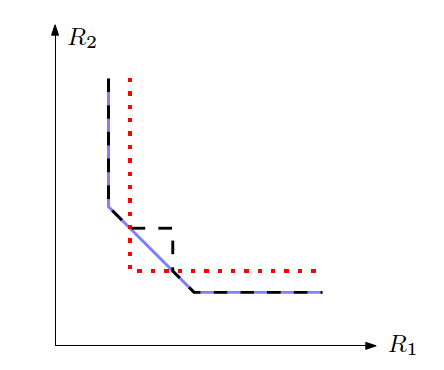
\includegraphics[width=0.45\textwidth]{nlc.png}
	\caption{两个信源基于嵌套线性码联合典型性译码的可达编码速率区域示例}
	\label{nlc}
\end{figure}
为了更清晰的阐述定理\ref{<theorem-chapter-2>}的可达速率区域，图\ref{nlc}给出了包含两个节点的系统，无损恢复一个线性组合的示例速率区域。其中，蓝色实线区域是SW可达速率区域，红色点线是Körner-Marton 可达速率区域，黑色虚线区域表示使用嵌套线性码独立恢复两个信源再进行线性计算的可达速率区域。定理\ref{<theorem-chapter-2>}可以实现Körner-Marton区域和黑色区域的并集，包含了SW区域，实现了比SW压缩更优的效果。

%\subsubsection{技术理论：嵌套线性码}
%嵌套线性码利用了有限域上线性码的群同态性质（Group Homomorphism）。一个嵌套线性码由一对线性码 $(\mathcal{C}_{\text{fine}}, \mathcal{C}_{\text{coarse}})$ 构成，满足 $\mathcal{C}_{\text{coarse}} \subset \mathcal{C}_{\text{fine}}$。其中 $\mathcal{C}_{\text{fine}}$（细码）用于保证信源的量化或覆盖，而 $\mathcal{C}_{\text{coarse}}$（粗码）用于实现分箱压缩。
%
%\begin{itemize}
%	\item \textbf{编码}：源节点 $k$ 将其观测数据序列映射到细码中的码字，并计算该码字相对于粗码的\textbf{伴随式（Syndrome）}或陪集索引。
%	\item \textbf{计算}：由于线性码的代数封闭性，接收端收到的多个伴随式的线性组合，恰好等于目标线性函数对应数据的伴随式。
%	\item \textbf{解码}：接收端直接对目标函数的伴随式进行解码，恢复出函数值。
%\end{itemize}
%
%\begin{theorem}[线性函数计算的可达速率界]
%	假设需要通过分布式网络计算 $K$ 个信源的线性组合 $Z = \sum_{k=1}^{K} c_k Y_k$，其中 $c_k$ 为有限域上的系数。若采用具有相同代数结构的嵌套线性码，当所有参与节点的编码速率 $R$ 满足以下条件时，接收端可以无损恢复目标函数 $Z$：
%	\begin{equation}
%		R \geq H(Z) = H\left(\sum_{k=1}^{K} c_k Y_k\right)
%	\end{equation}
%	更一般地，对于分布式线性函数计算问题，Körner-Marton 区域 $\mathcal{R}_{KM}$ 指出，只要速率满足以下条件即可实现函数恢复：
%	\begin{equation}
%		R_k \geq H\left(\sum_{k=1}^{K} c_k Y_k\right), \quad \forall k \in \{1, \dots, K\}
%	\end{equation}
%\end{theorem}
%
%\subsubsection{性能对比与意义}
%相较于 SW 编码，代数编码在特定场景下具有巨大的优势。例如，当两个二进制信源 $Y_1, Y_2$ 相互独立且均匀分布，但我们需要计算其模 2 和 $Z = Y_1 \oplus Y_2$ 时：
%\begin{itemize}
%	\item \textbf{SW 编码}：需恢复 $Y_1$ 和 $Y_2$，总速率 $R_{\text{sum}} \ge H(Y_1, Y_2) = 2$ bit。
%	\item \textbf{代数编码}：仅需恢复 $Z$，每个节点发送速率 $R \ge H(Z) = 1$ bit 即可（若利用广播特性可更低）。
%\end{itemize}

%在编码边缘计算中，这意味着如果任务是梯度聚合（求和），我们可以利用数据的线性结构，使得下行通信开销仅与模型参数维度相关，而与参与计算的边缘节点数量解耦，从而极大地提升大规模分布式系统的扩展性。

\section{NOMA}
% 作为5G、6G通信中的关键多址技术\cite{6G_NOMA_JEIT,NOMA6G_COMST}，
在编码计算场景中，当边缘节点完成计算任务后，需要通过下行无线信道将计算结果回传给中心节点进行恢复原始计算结果。为了提升频谱效率，下行传输考虑采用非正交多址接入技术（Non-Orthogonal Multiple Access，NOMA），采用其他多址接入技术也同样适用（如速率分割多址接入\upcite{9831440}）。
针对下一代无线通信系统对高频谱效率与海量连接的需求，非正交多址接入技术作为一种突破传统正交多址（OMA）资源分配范式的方案，受到了学术界和工业界的广泛关注\upcite{8357810}。根据资源映射方式的不同，NOMA主要分为功率域非正交多址（Power-Domain NOMA，PD-NOMA）\upcite{161197}、多用户共享接入（Multi-User Shared Access， MUSA）\upcite{170618}等。
PD-NOMA的核心思想在于通过在发射端引入叠加编码（Superposition Coding，SC），使多个用户共享同一时频资源块，并利用不同用户间信道增益的差异进行功率复用。在接收端，则采用相继干扰消除（Successive Interference Cancellation，SIC）技术，按照信号功率强度或者信道质量顺序逐层解码，从而有效缓解多用户干扰，如图\ref{noma}所示。本文后续研究均基于PD-NOMA展开（以下简称NOMA）。

\begin{figure}[htbp]
	\centering
	
\includegraphics[width=0.75\textwidth]{NOMA.png}
	\caption{功率域NOMA示意图}
	\label{noma}
\end{figure}
考虑一个包含$N$个边缘节点的编码计算场景，当计算较快的$K$个节点完成计算后，向中心节点下行传输计算结果，记第$k$个节点发射的信号为$s_k$，其发射功率为$p_k$。中心节点接收到的叠加信号为
\begin{equation}
	y=\sum_{k=1}^K \sqrt{p_k}h_ks_k+n_w,
\end{equation}
其中，$h_n$表示第$k$个边缘节点到中心节点的信道系数，$n_w \sim \mathcal{C}\mathcal{N}(0,\sigma^2)$为加性高斯白噪声（Additive Gaussian White Noise，AWGN）。

在接收端，中心节点根据各路信号的发射功率和信道系数升序（或降序）执行SIC检测，不失一般性，假设节点间的信道增益满足
\begin{equation}
	|h_1|^2p_1\geq |h_2|^2p_2\geq \cdots \geq |h_K|^2p_K.
\end{equation}
中心节点首先解码信号$s_1$，并将其余用户信号视作干扰。在解调出$s_k$后，中心节点从总接收信号中重构并减去该分量，再进行下一级解码。在理想SIC条件下，第$k$个用户所能达到的信息传输速率为
\begin{equation}
	R_k = B\log_2\left(1+\frac{p_k|h_k|^2}{N_0B+\sum_{i=k+1}^{K}p_i|h_i|^2}\right),
\end{equation}
其中$B$为带宽，$N_0$为背景噪声功率谱密度。

\section{凹凸过程与差分凸规划理论}

在编码边缘计算的资源分配优化问题中，由于无线信道的干扰特性以及通信与计算资源的耦合关系，目标函数或约束条件往往呈现出非凸特性。直接求解此类非凸优化问题通常是 NP-hard 的。凹凸过程（Convex-Concave Procedure, CCCP）作为一种处理差分凸（Difference of Convex, DC）规划问题的算法框架，能够将复杂的非凸问题转化为一系列凸优化子问题进行迭代求解，从而高效地收敛到局部最优解。本节将详细阐述其数学模型、核心原理及求解步骤。

具体来说，差分凸规划是一类特殊的非凸优化问题，其核心思想是任何非凸的目标函数或约束函数，往往可以表示为两个凸函数之差的形式。
考虑如下标准的非凸优化问题，
\begin{equation}
	\begin{aligned}
		\min_{\mathbf{x}} \quad & f_0(\mathbf{x}) \\
		\text{s.t.} \quad & f_i(\mathbf{x}) \leq 0, \quad i = 1, \dots, m,
	\end{aligned}
\end{equation}
其中 $\mathbf{x} \in \mathbb{R}^n$ 为优化变量。若函数 $f_i(\mathbf{x})$ ($i=0,\dots,m$) 可以分解为两个凸函数 $g_i(\mathbf{x})$ 和 $h_i(\mathbf{x})$ 的差，即
\begin{equation}
	f_i(\mathbf{x}) = g_i(\mathbf{x}) - h_i(\mathbf{x}),
\end{equation}
其中 $g_i: \mathbb{R}^n \rightarrow \mathbb{R}$ 和 $h_i: \mathbb{R}^n \rightarrow \mathbb{R}$ 均为凸函数，则该问题被称为差分凸规划问题，标准形式如下
\begin{equation}
	\label{eq:dc_standard}
	\begin{aligned}
		\min_{\mathbf{x}} \quad & g_0(\mathbf{x}) - h_0(\mathbf{x}) \\
		\text{s.t.} \quad & g_i(\mathbf{x}) - h_i(\mathbf{x}) \leq 0, \quad i = 1, \dots, m.
	\end{aligned}
\end{equation}
%例如，在通信系统中，常见的香农容量公式或信干噪比（SINR）约束通常符合 DC 结构，$\log(1+\text{SINR})$ 形式的非凸函数可以拆解为：
%\begin{equation}
%	\log\left(1 + \frac{S}{I+N}\right) = \underbrace{\log(S+I+N)}_{\text{凹函数}} - \underbrace{\log(I+N)}_{\text{凹函数}}.
%\end{equation}

对于DC问题的优化，可以采用CCCP算法。CCCP 的核心原理基于凸分析中的一阶泰勒展开和最大化-最小化（Majorization-Minimization, MM）思想。其主要方法是保持 DC 结构中的凸部分 $g_i(\mathbf{x})$ 不变，而对非凸部分（即减去的凸函数 $-h_i(\mathbf{x})$）进行线性化处理。
根据凸函数的性质，对于任意可微的凸函数 $h(\mathbf{x})$，其一阶泰勒展开构成了该函数的全局下界（Global Lower Bound）。即对于任意点 $\mathbf{x}^{(k)}$，有
\begin{equation}
	h(\mathbf{x}) \geq h(\mathbf{x}^{(k)}) + \nabla h(\mathbf{x}^{(k)})^T (\mathbf{x} - \mathbf{x}^{(k)})
\end{equation}
其中 $\nabla h(\mathbf{x}^{(k)})$ 表示函数在点 $\mathbf{x}^{(k)}$ 处的梯度。
在 CCCP 的第 $k$ 次迭代中，需要寻找原问题的一个凸近似。由于 $-h_i(\mathbf{x})$ 是凹函数，利用上述不等式，可以得到 $-h_i(\mathbf{x})$ 的一个全局线性上界
\begin{equation}
	-h_i(\mathbf{x}) \leq -\left[ h_i(\mathbf{x}^{(k)}) + \nabla h_i(\mathbf{x}^{(k)})^T (\mathbf{x} - \mathbf{x}^{(k)}) \right]
\end{equation}
定义线性化后的近似函数为 $\hat{h}_i(\mathbf{x}; \mathbf{x}^{(k)})$：
\begin{equation}
	\hat{h}_i(\mathbf{x}; \mathbf{x}^{(k)}) \triangleq h_i(\mathbf{x}^{(k)}) + \nabla h_i(\mathbf{x}^{(k)})^T (\mathbf{x} - \mathbf{x}^{(k)})
\end{equation}
通过将原 DC 问题 \eqref{eq:dc_standard} 中的所有 $h_i(\mathbf{x})$ 替换为其一阶近似 $\hat{h}_i(\mathbf{x}; \mathbf{x}^{(k)})$，可以构造出第 $k$ 次迭代的凸优化子问题：
\begin{equation}
	\label{eq:cccp_subproblem}
	\begin{aligned}
		\mathbf{x}^{(k+1)} = \arg \min_{\mathbf{x}} \quad & g_0(\mathbf{x}) - \hat{h}_0(\mathbf{x}; \mathbf{x}^{(k)}) \\
		\text{s.t.} \quad & g_i(\mathbf{x}) - \hat{h}_i(\mathbf{x}; \mathbf{x}^{(k)}) \leq 0, \quad i = 1, \dots, m
	\end{aligned}
\end{equation}

由于 $g_i(\mathbf{x})$ 和 $\hat{h}_i(\mathbf{x}; \mathbf{x}^{(k)})$ 是凸函数，因此上述子问题的目标函数和约束条件均为凸函数，可以利用标准的凸优化工具（如内点法等\upcite{boyd2004convex, potra2000interior}）求解该子问题。
由于CCCP算法会阐述一个解序列$\{\mathbf{x}^{(0)},\mathbf{x}^{(1)}\cdots\}$，并且优化过程中每一步都用函数的上界来近似目标函数和约束函数，根据 MM 算法理论，该序列的目标函数值是单调非递增的，即
\begin{equation}
	f_0(\mathbf{x}^{(k+1)}) \leq f_0(\mathbf{x}^{(k)})
\end{equation}
对于原问题的目标函数有下界的情况，CCCP的算法保证了收敛性，并且CCCP 通常收敛到原非凸问题的一个驻点，即满足 Karush-Kuhn-Tucker (KKT) 条件的局部最优解 \cite{7547360}。

%\subsection{算法步骤与收敛性}
%
%基于上述原理，CCCP 求解非凸优化问题的标准步骤如下：
%
%\begin{enumerate}
%	\item \textbf{初始化}：选择一个初始可行点 $\mathbf{x}^{(0)}$，设定容忍误差 $\epsilon > 0$ 和最大迭代次数 $L_{max}$，置迭代计数器 $k=0$。
%	\item \textbf{凸化近似}：在当前点 $\mathbf{x}^{(k)}$ 处，计算所有非凸项 $h_i(\mathbf{x})$ 的梯度 $\nabla h_i(\mathbf{x}^{(k)})$。
%	\item \textbf{求解子问题}：构造并求解凸优化子问题 \eqref{eq:cccp_subproblem}，得到新的最优解 $\mathbf{x}^{(k+1)}$。
%	\item \textbf{收敛判断}：检查收敛条件 $\|\mathbf{x}^{(k+1)} - \mathbf{x}^{(k)}\| \leq \epsilon$ 或目标函数值的变化量是否小于阈值。若满足条件，则停止迭代并输出 $\mathbf{x}^* = \mathbf{x}^{(k+1)}$；否则，令 $k \leftarrow k+1$，返回步骤 2。
%\end{enumerate}




\section{本章小结}

本章系统阐述了支撑本文研究的核心理论与关键技术，为后续章节中提出的编码结构适配传输机制奠定了坚实的理论基础。
首先，介绍了编码边缘计算的基本原理，重点分析了MDS码和梯度编码（在缓解分布式计算迟滞效应中的作用。分析表明，虽然任务编码引入了计算冗余，但也使得不同边缘节点的计算结果之间产生了强相关性，这为通信环节的优化提供了物理前提。
其次，深入探讨了DSC理论。通过对比传统的独立信源编码，阐述了面向完整数据恢复的 Slepian-Wolf 定理以及面向线性函数计算的嵌套线性码（基于 Körner-Marton 定理）。这部分理论揭示了如何利用计算结果间的相关性或代数结构来逼近数据压缩的理论极限，从而降低通信开销。
再次，介绍了非正交多址接入（NOMA）技术。作为一种高效的物理层传输手段，NOMA 允许利用功率域复用实现多节点的并发传输，能够有效提升下行链路的频谱效率和连接密度。
最后，详细描述了差分凸规划（DC Programming）模型及凹凸过程（CCCP）算法。针对编码边缘计算中通信与计算资源深度耦合所导致的非凸优化难题，CCCP 提供了一套收敛性良好且高效的数学求解框架。
综上所述，编码计算产生的结构化数据、分布式信源编码提供的压缩理论、NOMA 提供的高效传输手段以及 CCCP 提供的优化方法，共同构成了本文的研究基石。在接下来的章节中，本文将基于上述理论，分别针对通用数据完整重构场景（第三章）和特定线性函数聚合场景（第四章），展开具体的传输机制设计与性能优化研究。
\chapter{面向独立恢复的DSC辅助编码计算结果传输方法研究} \label{chapter-location-information}

\section{引言}

 分布式边缘计算通过将计算能力下沉到网络边缘，利用多个边缘节点并行处理计算任务，显著降低了端到端的计算时延，成为突破算力瓶颈的关键技术\upcite{gong2020delay}。
然而，分布式系统的性能往往受限于迟滞效应，即系统的整体完成时间取决于计算速度最慢的节点\upcite{ng2021comprehensive}。由于边缘节点的硬件配置、负载状态以及网络环境存在高度异构性，部分节点可能会因资源竞争或突发故障等随机因素导致计算停滞，从而严重拖累整个任务的完成进度。为了缓解这一问题，编码计算应运而生\upcite{ng2021comprehensive,9155226}。受经典纠错码理论的启发，编码边缘计算通过在任务分发阶段引入计算冗余，将原始任务编码为多个具有冗余特性的子任务。这种机制使得移动设备无需等待所有节点完成，仅需收集部分计算最快节点的计算结果即可恢复原始任务，从而有效缓解了迟滞节点的影响。

尽管编码边缘计算在提升计算效率方面上取得了显著进展，但现有的研究大多聚焦于设计高效的计算编码方案（如MDS码、梯度编码等）以降低计算延迟\upcite{8002642,peng2020diversity,9252114,tandon2017gradient,8758338}，而往往忽视了无线通信环节的挑战。具体而言，各边缘节点的计算结果回传过程同样面临着信道衰落、带宽受限等问题。如果参与回传的节点处于深衰落或拥塞信道中，通信延迟可能远超计算延迟，进而成为系统新的性能瓶颈。针对这一问题，部分近期工作开始探索计算与通信的联合优化策略\upcite{9046826,9829189,9328810,9820783}，例如通过调整任务分块大小、优化节点选择或设计协作传输机制。然而，这些工作通常将边缘节点的下行传输视为传统的多用户独立通信问题，即假设各节点发送的消息是相互独立的。
事实上，编码边缘计算与传统多用户通信存在本质区别：由于在任务分发阶段采用了纠删码技术，不同边缘节点计算出的中间结果之间存在着内生的强相关性。这种相关性蕴含了巨大的通信优化潜力，却在现有研究中被长期忽视。从信息论的角度来看，这一场景与经典的分布式信源编码问题具有天然的同构性：多个相关信源在不进行相互通信的情况下，分别向同一接收端发送信息\upcite{1055037,1328091}。在编码计算中，如果边缘节点能够利用DSC技术来压缩计算结果，并重新分配节点间的传输负载以更好地匹配信道条件，那么将可能实现更高效的下行传输。

DSC的相关研究可以追溯到文献\upcite{1055037}的开创性工作，并由此引发了一系列的进一步研究，例如多信源场景\upcite{1055356,1281474,1614079}，异步场景\upcite{5407617,7360786}以及有损恢复问题\upcite{1055508,4475358}。然而，许多早期DSC工作中考虑的编码方法主要具有理论意义，在实际应用中可能并不适用。因此，许多近期关于DSC的研究开始转向实用编码方案的设计\upcite{1614079, 1184140,6241374,4494710,1365367,1375242,4697499}。这些研究通过探索DSC与信道编码之间的关系\upcite{1328091}，并基于伴随式\upcite{1184140}进行解码。大多数此类研究集中于两个相关信源的编码设计\upcite{1365367,1375242,4697499}，并且只能达到SW区域的角点。对于一般的非二进制多信源场景，设计能够实现整个SW区域编码速率范围的实用方案仍然是一个挑战。现有的研究要么压缩效果是次优的，要么仅适用于特定的信源\upcite{6241374,6685982,1042242}，或者往往在实现上面临极高的复杂度\upcite{1281474,1661834}。此外，这些现有的DSC相关工作主要针对通用的相关信源模型，而利用编码计算的特性设计高效的DSC方面的研究目前仍然缺失。


基于上述观察，本章提出了一种基于DSC辅助的编码计算结果下行传输机制。旨在利用编码任务间的相关性，打破传统独立传输的性能界限。具体而言，本章的主要贡献如下：
深入分析了MDS编码计算任务在边缘节点间引入的代数相关性，并将其建模为分布式相关信源。结合非正交多址接入技术（NOMA）\upcite{8357810}，构建了DSC辅助的下行传输系统模型。
针对SW定理缺乏实用编码方案的问题，设计了一种基于LDPC码的伴随式穿刺传输方法。该方法允许边缘节点根据自身信道状态自适应地调整压缩率，即调整传输的伴随式长度，从而实现传输负载在节点间的灵活重分配，有效缓解了信道条件差的节点对系统性能的制约。
建立了基于DSC的下行传输时延最小化问题。针对该问题的非凸特性，利用差分凸规划理论，提出了一种基于连续凸逼近的迭代优化算法，联合优化各节点的信源压缩率与发射功率。

本章后续内容安排如下：3.2节详细描述系统模型与问题建模；3.3节介绍所提的伴随式穿刺传输方案及DSC解码流程；3.4节阐述基于CCCP的时延优化算法；3.5节通过仿真实验验证所提方案的有效性；3.6节对本章进行总结。表\ref{<chapter-three-table-symbols>}列出了本章的常用符号。
\begin{table}[htbp]
	%\small
	\centering
	\caption{本章常用符号}
	\begin{tabular}{c p{28em}}
		\toprule
		符号 & 含义\\
		\midrule
		$k$ & 边缘节点数目 \\
		$r$ & 划分的子任务数目 \\
		$\mathcal{J}$&参与下行传输的边缘节点集合\\
		$X_i$ & 未编码子任务$i$的计算结果 \\
		$Y_i$ & 编码子任务$i$的计算结果 \\
		$S_{Y_i}$& 编码子任务$i$的计算结果对应生成的伴随式\\
		$S_{X_i}$& 未编码子任务$i$的计算结果对应生成的伴随式\\
		$\tilde{\eta}$ & 直接信源编码的压缩率 \\
		$\bar{\eta}$ & 理想信源编码的压缩率\\
		$\eta$ & 基于伴随式穿刺的实际信源编码的压缩率\\
		$s$ & 每个节点需要传输的符号数 \\
		$T_d$ & 下行传输所需时延 \\
		$P_{\text{max}}$ & 边缘节点的最大传输功率 \\
		$\symbfit{g}_i$ & 移动设备与边缘节点$i$间的信道增益 \\
		$B$ & 下行信道带宽 \\
		$n_0$ & 信道噪声功率谱密度 \\        
		\bottomrule
	\end{tabular}
	\label{<chapter-three-table-symbols>}
\end{table}


\section{系统模型与问题建模}

	考虑如图\ref{cdc}所示的编码计算场景，其中包含一个移动设备与$k$个边缘节点。由于这$k$个节点可能会存在迟滞现象，采用$(k,r)$线性分组码对计算任务进行编码分发\upcite{ng2021comprehensive}。具体来说，假设每个原始计算任务被划分为$r$个相互独立的子任务。随后，采用$(k,r)$线性分组码对原始任务进行编码，生成$k$个编码子任务并分发给边缘节点并行处理。
	\begin{figure}[htbp]
		\centering
		%	\setlength{\abovecaptionskip}{-0.1cm}
		\includegraphics[width = 0.67\textwidth]{codededgecomputing.pdf}
		\DeclareGraphicsExtensions.
		\caption{编码计算系统模型}
		%			, and $\mathcal{J}_1=\{1,3,4\}, ~\mathcal{J}_2=\{1,2,4\}, ~\mathcal{J}_3=\{1,2,3\}, ~\mathcal{J}_4=\{2,3,4\}$.}
	\label{cdc}
	\end{figure}
	
\subsection{编码计算模型}
	假设这些未编码子任务和编码子任务的计算结果为取自有限域$GF(q)$上的随机变量，分别记为$\{X_i\}_{i=1}^r$和$\{Y_i\}_{i=1}^k$。当采用线性编码时，第$i$个边缘节点的计算结果$Y_i$建模为原始子任务的线性组合，即
\begin{equation}
	Y_i=\sum\nolimits_{j=1}^{r}\varphi_{i,j}X_j, ~\forall i\in[k]\label{yx},
\end{equation}其中$\varphi_{i,j}$是编码系数。假设$r$个未编码子任务的计算结果$X_i$'s 服从独立同分布\upcite{9229375}，且熵由$H(X)$表示。由于编码后的子任务$Y_i$'s 是$X_i$'s 的线性组合，可以证明$k$个编码子任务的信息熵满足$H(Y_i)\geq H(X),~\forall i\in[k]$。

考虑在计算阶段完成时，只有$\mathcal{J}\subseteq[k]$个非迟滞节点完成了计算任务。在下行传输阶段，由这些已经完成计算任务的节点将计算结果传输给移动设备。根据编码计算的特性，移动设备在收到任意$r$个或更多节点的计算结果后就能够重新构建出每个未编码子任务的计算结果$X_i$，即
\begin{equation}
	X_i=\sum\nolimits_{\upsilon=1 }^r \beta_{i,j_\upsilon} Y_{j_\upsilon},~\forall i\in[r],\label{linear_re}
\end{equation}
其中$\{j_1,\cdots,j_r\}\subset\mathcal{J}$且$\beta_{i,j_\upsilon}$'s 是相应的解码系数且可以通过(\ref{yx})唯一的确定。在构建出$r$个未编码子任务的计算结果后，移动设可以恢复原始计算任务的计算结果。


为了提升计算结果$Y_i$'s 的传输效率，许多无线通信系统中将采取信源编码无损压缩这些计算结果\upcite{doi:https://doi.org/10.1002/047174882X.ch15}，再将压缩后的计算结果回传给移动过设备。现有一些编码计算的工作中，各个边缘节点被视为独立信源，采用独立的信源编码方式\upcite{ng2021comprehensive} 。假设对每个节点，最直接的信源编码方式是按照自身无损恢复所需的最小信息量独立地对计算结果进行压缩和传输。因此，根据经典信源编码定理，对于节点$i$的计算结果，用$n$长的序列表示，记为$\left\{Y_i^{(j)}\right\}_{j=1}^n$，其中$n$足够大。该序列可以被压缩为更短的序列$\left\{\tilde{S}_{Y_i}^{(j)}\right\}_{j=1}^{\tilde{m}_i}$，长度为$\tilde{m}_i=\frac{n H(Y_i)}{\log_2 q}$, 其中 $Y_i^{(j)}$和$\tilde{S}_{Y_i}^{(j)}$分别表示序列里相应的第$j$个符号，便于理解，序列$\left\{Y_i^{(j)}\right\}_{j=1}^n$和$\left\{\tilde{S}_{Y_i}^{(j)}\right\}_{j=1}^{\tilde{m}_i}$的向量形式记为$\mathbf{Y}_i^{1:n}$和$\mathbf{\tilde{S}}_{Y_i}^{1:\tilde{m}_i}$， 对应的信源压缩率可以表示为
\begin{equation}
	\setlength\belowdisplayskip{3pt}
	\tilde{\eta_i}=\frac{H(Y_i)}{\log_2q},~\forall i\in\mathcal{J}.\vspace{0.03cm}\label{straight}
\end{equation}

\subsection{下行传输模型}\label{communication model}
在下行传输过程中，为了提升传输效率，在现有的一些编码计算工作中\upcite{ng2021comprehensive}，通常会选取信道条件最好的$r$个节点满足$\tilde{\mathcal{J}}\subseteq\mathcal{J}$将它们压缩后的计算结果$\left\{\tilde{S}_{Y_i}^{(j)}\right\}_{j=1}^{\tilde{m}_i}$回传给移动设备。
为了提升频谱效率并支持并行传输，这些$r$个节点将采用非正交多址的方案进行传输。本研究中将采用功率域NOMA\upcite{8357810}作为示例，移动设备接收叠加信号后，按照信道增益由强到弱的顺序执行串行干扰消除，对于第$i$个解码的节点，来自信道更差节点的信号被视为干扰，而信道更好的节点信号假设已被消除，采用其他的多址传输方案例如RSMA也适用于本研究 \upcite{9831440} 。为了不失一般性，假设这$|\mathcal{J}|$个成功完成计算任务的节点其信道增益$g_i$'s 按照降序排列$g_1\geq g_2\geq \cdots \geq g_{|\mathcal{J}|}$，其中为了便于理解，这些节点也按照$1$到$|\mathcal{J}|$表示。因此，节点1到节点$r$将被选取参与下行传输。根据文献\cite{8357810}，第$i$个边缘节点的下行可达速率$R_i$可以表示为
\begin{equation}
	R_i=B\log_2\left(1+\frac{g_ip_i}{Bn_0+\sum_{j=i+1}^{r}g_jp_j}\right)\label{sic},~\forall i\in\tilde{\mathcal{J}},
\end{equation}
其中$p_i$表示节点$i$的发射功率，$B$表示下行传输的带宽，$n_0$表示噪声功率。

为了保证下行传输成功，这些$r$个节点的信源压缩率$\eta_i$'s 和传输速率$R_i$'s 需要满足
\begin{equation}
	R_{i}T_d\geq  \tilde{\eta_i} s\log_2q, ~ \forall i\in \tilde{\mathcal{J}},\label{rt>r'}
\end{equation}
其中$T_d$表示下行传输延迟，$s$表示每个节点未压缩前需要传输的计算结果包含的符号数。

本研究的主要目标是降低下行传输延迟$T_d$。然而，基于直接信源编码方法及公式（\ref{rt>r'}），如果在这$r$个被选中的边缘节点中，仍有一个节点的信道条件较差，从而导致传输速率 较低，那么该节点将成为瓶颈，并可能严重延长下行传输延迟$T_d$。为了缓解这种情况可能造成的下行传输延迟，本研究将提出基于DSC辅助的编码计算结果下行传输方案。

\subsection{面向独立恢复的 DSC 辅助传输机制}
为了激发所提出的方案，首先注意到在第 \ref{communication model}节描述的基于独立压缩的传输方案中，如果某个节点的信道非常差，整体传输延迟 $T_d$ 将受到此瓶颈的限制（见\ref{rt>r'}）。这是因为在直接方法中，节点的传输信息是独立压缩的.尽管其他节点可能拥有良好的信道，但它们没有信道较差节点的信息，因此无法提供帮助。理想情况下，如果信道较差的节点的传输负载能够被重新分配给信道良好的节点（且不产生额外的通信开销），这个问题就可以得到解决。幸运的是，当 $|\mathcal{J}| > r$ 时，这实际上是可能的，因为由于任务编码的存在，节点的计算结果是相关的（因为任意 $r$ 个 $Y_i$ 足以根据公式 (\ref{linear_re}) 唯一确定所有的 $X_i$。由于多个节点之间的信息存在冗余，而传统的信源编码方案并没有将这部分冗余信息去除，而是进行独立信源编码并传输计算结果。此外，传统的传输方式，只选取了计算较快的$r$个节点进行传输，如果其中一个节点的信道条件很差，这将会导致传输延迟的增大，从而造成整体端到端延迟的增加。如果采取$|\mathcal{J}|~(\geq r)$个完成计算的节点同时参与下行传输，且传输负载可以灵活分配，可以达到信道条件好的节点多传数据，信道条件差的节点少传部分数据的效果，从而实现整体传输效率的提高。而在分布式信源编码中，多个相关信源之间互相不通信进行信源，在接收端执行联合译码可以无损恢复所有信源。在信源压缩和解码的过程可以看成是负载重分配的一个过程。
因此，所需的负载重分配实际上可以通过 DSC来实现\upcite{1055037,1055356}，具体阐述如下。

\subsubsection{DSC 辅助传输模型}
在提出的方案中，所有完成计算的 $|\mathcal{J}|$ 个 节点都将参与下行传输，并利用 DSC 压缩其计算结果。具体而言，每个节点 $i \in \mathcal{J}$ 将其长度为 $n$ 的计算结果序列 $\{Y_i^{(j)}\}_{j=1}^n$ 以目标压缩率 $\bar{\eta}_i$压缩为长度为 $\bar{m}_i = n\bar{\eta}_i$ 的更短序列 $\{\bar{S}_{Y_i}^{(j)}\}_{j=1}^{\bar{m}_i}$，其中目标压缩率 $\bar{\eta}_i$将通过优化确定。理论上，通过理想的信源编码方案（经由随机分箱），任何满足公式 (\ref{sw}) 的压缩率集合 $\{\bar{\eta}_i\}_{i=1}^{|\mathcal{J}|}$ 都是可达的\upcite{1055037,1055356}，经典的SW定理给出了压缩率的可达区域，即
\begin{align}
	\sum\nolimits_{i\in \mathcal{L}}\bar{\eta}_{i}\geq \frac{H(Y_{\mathcal{L}}|Y_{\mathcal{L}^C})}{\log_2q}, ~\forall \mathcal{L}\subseteq \mathcal{J},\label{sw}
\end{align}。
其中$\mathcal{L}^C$ 表示 $\mathcal{L}$ 相对于 $\mathcal{J}$的补集,  $\bar{\eta}_{i}$表示$Y_i$的压缩率。
在 DSC 的辅助下，节点现在可以通过使用不同的压缩率 $\bar{\eta}_i$ 来灵活调整其传输负载。例如，信道较差的节点可以选择较小的压缩率（传输较少的信息），而信道较好的节点 可以采用较大的压缩率（传输更多的信息），只要满足公式 (\ref{sw}) 即可。从某种意义上说，这相当于在不产生额外通信的情况下，将部分传输负载从信道较差的 节点重新分配给了信道较好的节点。凭借这种传输负载重分配的灵活性，上述瓶颈问题得以缓解，从而实现更短的下行传输延迟 $T_d$（参考公式 (\ref{rt>r'})）。然而经典SW定理只适用于理论研究，在实际中难以实现SW可达区域\upcite{1328091}。为此，下一小节提出了一种更实用的基于伴随式穿刺的 DSC 方法。


\subsubsection{基于伴随式穿刺的实用DSC方案}

为了能更好的实现信源压缩，利用编码计算的固有特性，本研究设计了一种基于LDPC码的低复杂度信源编码方案。具体而言，该方案包括三个主要步骤，分别是伴随式生成，伴随式穿刺以及伴随式恢复。如图\ref{dsc}所示，为了达到目标压缩率$\eta_i$'s，每个节点首先根据$\left\{Y_i^{(j)}\right\}_{j=1}^n$生成长度为$m=\frac{nH(X)}{\log_2q}$的序列$\left\{S_{Y_i}^{(j)}\right\}_{j=1}^m$。随后，执行伴随式穿刺，使得每个 EN $i$ 只需要传输生成伴随式的一个子集 $\{S_{Y_i}^{(j)}\}_{j \in \Pi_i}$，其中 $\Pi_i \subseteq [m]$ 表示需由 EN $i$ 传输的伴随式的索引集合。这一步的主要目的是进一步降低压缩率，并允许（根据传输速率 $R_i$）自适应地调整压缩率。在伴随式恢复步骤中，移动设备利用接收到的伴随式 $\{S_{Y_i}^{(j)}\}_{j=1}^m (\forall i \in \mathcal{J})$ 重构未编码子任务计算结果 $\{X_v^{(j)}\}_{j=1}^n$ 的伴随式 $\{S_{X_v}^{(j)}\}_{j=1}^m$。注意，由于编码计算假设了线性关系 (\ref{yx})，这种伴随式恢复是可能的。此后，采用（基于伴随式的）置信传播 (BP) 译码算法\upcite{4697499,1042242}从 $\{S_{X_v}^{(j)}\}_{j=1}^m$ 中解码出 $\{X_v^{(j)}\}_{j=1}^n$。详细步骤如下。

\begin{figure}[!t]
\centering
%	\setlength{\abovecaptionskip}{-0.1cm}
\includegraphics[width = 1.03\textwidth]{figs/syn.pdf}
\DeclareGraphicsExtensions.
\caption{所提分布式信源编码方案图示}
%			, and $\mathcal{J}_1=\{1,3,4\}, ~\mathcal{J}_2=\{1,2,4\}, ~\mathcal{J}_3=\{1,2,3\}, ~\mathcal{J}_4=\{2,3,4\}$.}
\label{dsc}
\end{figure}

（1）伴随式生成：在此步骤中，利用 LDPC 码，从计算结果 $\mathbf{Y}_i^{1:n}$ 生成伴随式 $\mathbf{S}_{Y_i}^{1:m}$，如下所示：

\begin{equation}
\mathbf{S}_{Y_i}^{1:m}=\mathbf{Y}_i^{1:n}\mathbf{H}^{n\times m}, ~\forall i\in\mathcal{J},\label{sy}
\end{equation}
其中校验矩阵 $\mathbf{H}^{n \times m}$ 的元素取值于有限域 $GF(q)$，LDPC 码率\upcite{1057683}设定为 $\eta_c = \frac{n-m}{n} = 1 - \frac{H(X)}{\log_2 q}$。

（2）伴随式穿刺：在提出的方案中，为了实现更好的压缩，每个节点只传输由公式 (7) 生成的伴随式的一部分，其余部分被穿刺。特别是，对于给定的一组压缩率 $\{\eta_i\}_{i=1}^{|\mathcal{J}|}$，由 EN $i$ 传输的连续伴随式的索引集合 $\Pi_i$ 由下式给出：

\begin{equation}
\Pi_i=\left\{\alpha_{i-1}\oplus_m 0+1,\alpha_{i-1}\oplus_m 1+1,\cdots,\alpha_i\right\},\label{Pi}~\forall i\in\mathcal{J}.
\end{equation}
其中，$\oplus_m$表示对$m$做取余运算，$\alpha_i$表示节点$i$传输的最后一个数据下标索引，可以定义为
\begin{equation}
\alpha_i=\alpha_{i-1}\oplus_m(\lceil\eta_in\rceil-1)+1,~\forall i\in\mathcal{J},\label{split}
\end{equation} 
其中，$\alpha_0$定义为0，$\lceil \cdot \rceil$ 表示向上取整运算。为了便于理解，图\ref{fig3}提供了一个简单的伴随式穿刺示例，其中白色条表示被穿刺的伴随式。

\begin{theorem}\label{proposition1}
	在提出的编码下，如果目标压缩率 $\{\eta_i\}_{i=1}^{|\mathcal{J}|}$ 满足
	
	\begin{equation}
		\sum_{i=1}^{|\mathcal{J}|} \eta_i \geq \frac{rH(X)}{\log_2 q},
		\label{eq:prop_cond1}
	\end{equation}
	\begin{equation}
		0 \leq \eta_i \leq \frac{H(X)}{\log_2 q}, \quad \forall i \in \mathcal{J},
		\label{eq:prop_cond2}
	\end{equation}
	
	那么，对于每一个索引 $1 \leq j \leq m$，都存在一个（至少）大小为 $r$ 的集合 $\mathcal{J}_j$，使得对于所有 $i \in \mathcal{J}_j$，都有 $j \in \Pi_i$。
\end{theorem}
\begin{proof}
	详见附录 \ref{<appendix-proposition1>}。
\end{proof}

直观上，定理\ref{proposition1} 表明当 (\ref{eq:prop_cond1}) 和 (\ref{eq:prop_cond2}) 成立时，由 (\ref{Pi}) 和 (\ref{split}) 指定的伴随式穿刺步骤确保了对于每个索引 $j$，至少有 $r$ 个 节点传输了它们的第 $j$ 个伴随式。此外，不难验证，对应的集合 $\mathcal{J}_j$ 可以由 (\ref{eq:prop_cond1}) 中给出的索引集 $\Pi_i$ 唯一确定。注意，由于 $r$ 是底层编码计算机制的恢复阈值，这将使移动设备能够恢复未编码子任务结果的相应第 $j$ 个伴随式，如下面的伴随式恢复步骤所示。


（c）伴随式恢复：在此步骤中，通过调用公式 (\ref{linear_re}) 中的编码计算属性，从定理\ref{proposition1} 中给出的集合 $\mathcal{J}_j$ 中的 $r$ 个 EN 传输的伴随式中，恢复出 $r$ 个未编码子任务计算结果的伴随式 $S_{X_v}^{(j)}$。具体地，使用向量 $\mathbf{S}_{X_v}^{1:m}$ 来紧凑地表示对应于未编码子任务 $\mathbf{X}_v^{1:n}$ 的计算结果的伴随式 $\{S_{X_v}^{(j)}\}_{j=1}^m$，它满足

\begin{equation}
\mathbf{S}_{X_\upsilon}^{1:m}=\mathbf{X}_\upsilon^{1:n}\mathbf{H}^{n\times m},~\forall \upsilon\in[r],\label{sx}
\end{equation}
其中，$\mathbf{H}^{n\times m}$是（\ref{sy}）中的奇偶检验矩阵。将（\ref{linear_re}）两边同时乘以$\mathbf{H}^{n\times m}$并比较（\ref{sy}）和（\ref{sx}）可以得出伴随式$\left\{S_{X_\upsilon}^{(j)}\right\}_{j=1}^{m}$ 可以从接收到的伴随式$\left\{S_{Y_i}^{(j)}\right\}_{j=1}^{m}$ 中恢复，如下所示
\begin{equation}
S_{X_\upsilon}^{(j)}=\sum\nolimits_{i\in \mathcal{J}_j} \beta_{\upsilon,i}S_{Y_i}^{(j)},~ \forall \upsilon\in[r],~\forall j\in [m].\label{linear}
\end{equation}		
一旦恢复了所有的伴随式 $\left\{S_{X_v}^{(j)}\right\}_{j=1}^m (\forall v \in [r])$，就可以使用基于伴随式的 BP 算法\upcite{1042242, 4697499}解码出未编码子任务的计算结果 $\left\{X_v^{(j)}\right\}_{j=1}^n (\forall v \in [r])$。为了完整性，附录\ref{appendix-BP} 中给出了基于伴随式的 BP 算法的细节。

所提出的基于伴随式打孔的 DSC 方法的计算复杂度分析如下。
在编码阶段，伴随式生成步骤 (\ref{sy}) 和伴随式穿刺步骤 (\ref{split}) 的复杂度分别为 $O(mn|\mathcal{J}|)$ 和 $O(|\mathcal{J}|)$\upcite{706440}。在解码阶段，伴随式恢复步骤 (\ref{linear}) 和 BP 解码步骤的复杂度分别约为 $O(r^2m)$ 和 $O(n_{iter} n d_v q^2)$ ，其中 $n_{iter}$ 是 BP 算法的迭代次数，$d_v$ 是连接到每个变量节点的校验节点数。与3.2.2 部分描述的传统方法相比，所提出的方案仅在伴随式打孔和伴随式恢复步骤中引入了额外的复杂度，总计为 $O(|\mathcal{J}| + r^2m)$。由于 $m$ 与 $n$ 相当，这个额外的复杂度 $O(|\mathcal{J}| + r^2m)$ 与 BP 的单次迭代复杂度 $O(n d_v q^2)$ 相当。换句话说，所提出的编码引入的额外复杂度大致相当于只给 BP 算法增加了一次迭代，这通常只会导致下行链路复杂度的极小幅增加。

\begin{figure}[!t]
	\centering
	%	\setlength{\abovecaptionskip}{-0.1cm}
	
\includegraphics[width = 0.6\textwidth]{figs/fig5.eps}
	\DeclareGraphicsExtensions.
	\caption{伴随式穿刺图示，其中$\Pi_1=\{1,\cdots,\alpha_1\},~ \Pi_2=\{\alpha_1\oplus_m 0+1,\cdots,\alpha_2\}, ~\Pi_3=\{\alpha_2\oplus_m 0+1,\cdots,\alpha_3\}$,  $ \Pi_4=\{\alpha_3\oplus_m 0+1,\cdots,\alpha_4\}$}
	%			, and $\mathcal{J}_1=\{1,3,4\}, ~\mathcal{J}_2=\{1,2,4\}, ~\mathcal{J}_3=\{1,2,3\}, ~\mathcal{J}_4=\{2,3,4\}$.}
\label{fig3}
\end{figure}

\begin{corollary}
	上述提出的编码可以实现由 (\ref{eq:prop_cond1}) 和 (\ref{eq:prop_cond2}) 指定区域内包含的任何压缩率。
\end{corollary}

一般来说，所提出的编码的可达区域是理想 SW 可达区域的一个子区域。
为了便于感知，图 \ref{example}提供了一个示例，其中比较了所提出的编码（蓝色）和理想 SW 区域（绿色）的理论可达区域。注意，虽然所提出的编码仅实现了 SW 区域的一个子区域，但它在选择合适的压缩率以匹配 节点信道质量和重新分配传输负载方面仍提供了很大的灵活性，这使其能够大幅减少下行链路延迟。

\begin{figure}[htbp]
	\centering
	\setlength{\abovecaptionskip}{-0.1cm}
	\includegraphics[width = 0.75\textwidth]{figs/SW_region_example.eps}
	%		 where an .eps filename suffix will be assumed under latex, 
	%		 and a .pdf suffix will be assumed for pdflatex; or what has been declared
	\DeclareGraphicsExtensions.
	\caption{DSC可行区域的比较示例（其中 $\eta_c=0.5$, $q=64,~\frac{H(X)}{\log_2q}=0.5,~\frac{H(Y_i)}{\log_2q}=0.6~(\forall i\in\mathcal{J})$, $|\mathcal{J}|=3$, $r=2$）。}
	\label{example}
\end{figure}

\subsubsection{高维数据下的DSC辅助下行传输方案}

所提实际分布式信源编码方案可以扩展到多维数据的场景。具体而言，对于 $V$ 维数据，将 $r$ 个未编码子任务的计算结果和 $k$ 个编码子任务的计算结果分别表示为 $X_i = [X_{i1}, \cdots, X_{iV}], \forall i \in [r]$ 和 $Y_i = [Y_{i1}, \cdots, Y_{iV}], \forall i \in [k]$。边缘节点$i$的长度为$n$的编码结果可以表示为一个大小为$V\times n$的矩阵$\textbf{Y}_i^{1:n} = \left[Y_{i_v}^{(j)}\right]_{v\in[V],j\in[n]}$，其中$i\in\mathcal{J}$。为了处理这种高维数据，可以将逐级编码\upcite{5208477,4215156,coleman2006low}的思想与所提编码方法相结合，按顺序统一传输$\textbf{Y}_i^{1:n}$'s的每一行，总下行传输时延将是这些维度的传输时延之和。假设各维度将按照$1$到$V$的顺序进行压缩和传输。那么，对于每一个维度$v\in[V]$,可以应用上述所提的基于伴随式穿刺的分布式信源编码方法。在伴随式生成步骤中，所提方案将根据条件熵$H(X_{i_v}|X_{i_{v-1}},\cdots, X_{i_1})$，使用码率为$\eta_c=1-\frac{H(X_{i_v}|X_{i_{v-1}},\cdots, X_{i_1})}{\log_2 q}$的LDPC码，将序列$\left[Y_{i_v}^{(j)}\right]_{j\in[n]}$ 压缩为伴随式 $\left[S_{Y_{i_v}}^{(j)}\right]_{j\in[m]},~\forall i\in\mathcal{J}$。相应地，在置信传播译码算法中，所有的先验概率${\rm{Pr}} \{x_{i}=a\}$ 将更改为条件概率${\rm{Pr}} \{x_{i_v}=a|x_{i_{v-1}}\cdots x_{i_{1}}\},~\forall a\in GF(q)$。因为在假设的维度压缩和传输顺序下，前$v-1$个维度已经被成功解码，条件概率中$x_{i_{v-1}},\cdots,x_{i_1}$的值是已知的。

\subsubsection{DSC辅助的下行传输示例}
为了清晰起见，下面给出了所提出编码的一个简单示例。假设编码计算的恢复阈值为 $r = 2$，并且在计算阶段结束时有 $|\mathcal{J}| = 3$ 个 节点完成了计算。此外，假设 $H(X_1) = H(X_2) = 3$，并且已编码子任务的计算结果 $Y_1, Y_2$ 和 $Y_3$ 满足
\begin{subequations}\label{eq:toy}
	\begin{align}
		Y_1 &= X_1 + X_2, \label{eq:toy_y1} \\
		Y_2 &= X_1 + 2X_2, \label{eq:toy_y2} \\
		Y_3 &= X_1 + 3X_2, \label{eq:toy_y3}
	\end{align}
\end{subequations}
其中有限域为 $GF(64)$。在这个例子中，使用本原多项式 $x^6 + x + 1$ 进行域运算。此外，假设已编码子任务的计算结果 $\{Y_i\}_{i=1}^3$ 的目标压缩率 $\{\eta_i\}_{i=1}^3$ 分别为 $\eta_1 = 0.3, \eta_2 = 0.3$ 和 $\eta_3 = 0.4$。

为了执行所提出的 DSC，长度为 $n = 10$ 的计算结果序列 $\{Y_i^{(j)}\}_{j=1}^n$ 将被非二进制 LDPC 码压缩，码率为 $\eta_c = 1 - \frac{H(X)}{\log_2 q} = 0.5$。对应的奇偶校验矩阵假设为
\begin{equation}
	\mathbf{H}^{n \times m} =
	\begin{bmatrix}
		10 & 0 & 0 & 0 & 0 & 18 & 0 & 2 & 0 & 5 \\
		0 & 2 & 0 & 12 & 0 & 1 & 21 & 0 & 0 & 0 \\
		0 & 7 & 3 & 0 & 0 & 0 & 0 & 29 & 11 & 0 \\
		16 & 0 & 0 & 31 & 3 & 0 & 0 & 0 & 41 & 0 \\
		0 & 0 & 9 & 0 & 19 & 0 & 4 & 0 & 0 & 8
	\end{bmatrix}^T,
	\label{eq:toy_matrix}
\end{equation}
其中 $m = n(1 - \eta_c) = 5$。更具体地说，假设 $Y_1, Y_2$ 和 $Y_3$ 的符号序列如下
\begin{subequations}
	\begin{align}
		\mathbf{Y}_1^{1:n} &= [3, 7, 9, 7, 9, 5, 9, 11, 10, 5], \label{eq:toy_seq_y1} \\
		\mathbf{Y}_2^{1:n} &= [5, 10, 15, 8, 13, 8, 11, 18, 15, 9], \label{eq:toy_seq_y2} \\
		\mathbf{Y}_3^{1:n} &= [7, 13, 21, 9, 17, 11, 13, 25, 20, 13]. \label{eq:toy_seq_y3}
	\end{align}
\end{subequations}
根据 (\ref{sy})，生成的伴随式序列为
\begin{subequations}
	\begin{align}
		\mathbf{S}_{Y_1}^{1:m} &= [\underline{0}, \underline{20}, \underline{9}, 35, 3], \label{eq:toy_syn_y1} \\
		\mathbf{S}_{Y_2}^{1:m} &= [\underline{61}, 46, 46, \underline{36}, \underline{17}], \label{eq:toy_syn_y2} \\
		\mathbf{S}_{Y_3}^{1:m} &= [29, \underline{18}, \underline{47}, \underline{14}, \underline{11}]. \label{eq:toy_syn_y3}
	\end{align}
\end{subequations}
然后应用伴随式穿刺步骤，根据 (\ref{Pi})，这些 $|\mathcal{J}| = 3$ 个 节点将传输的伴随式 $\{S_{Y_i}^{(j)}\}_{j=1}^m (\forall i \in \mathcal{J})$ 的索引由下式给出
\begin{equation}
	\Pi_1 = \{1, 2, 3\}, \Pi_2 = \{4, 5, 1\}, \Pi_3 = \{2, 3, 4, 5\}.
	\label{eq:toy_indices}
\end{equation}
也就是说，只有 (\ref{eq:toy_syn_y3}) 中带有下划线的伴随式会被传输。根据 (\ref{eq:toy_indices})，对应的集合 $\mathcal{J}_j$ 如下给出
\begin{gather}
	\mathcal{J}_1 = \{1, 2\}, \mathcal{J}_2 = \{1, 3\}, \mathcal{J}_3 = \{1, 3\}, \nonumber \\
	\mathcal{J}_4 = \{2, 3\}, \mathcal{J}_5 = \{2, 3\}.
	\label{eq:toy_sets}
\end{gather}
为了重构未编码子任务计算结果的伴随式序列，(\ref{linear}) 中的系数 $\beta_{v,i}$ 可以根据 (\ref{eq:toy})、(\ref{eq:toy_indices}) 中给出的索引以及 (\ref{eq:toy_sets}) 中的对应集合来确定，从而得出
\begin{equation}
	S_{X_1}^{(j)} =
	\begin{cases}
		2S_{Y_1}^{(j)} - S_{Y_2}^{(j)}, & \text{for } j = 1, \\
		\frac{3}{2} S_{Y_1}^{(j)} - \frac{1}{2} S_{Y_3}^{(j)}, & \text{for } j = 2, 3, \\
		3S_{Y_2}^{(j)} - 2S_{Y_3}^{(j)}, & \text{for } j = 4, 5,
	\end{cases}
	\label{eq:toy_recover_x1}
\end{equation}
以及
\begin{equation}
	S_{X_2}^{(j)} =
	\begin{cases}
		S_{Y_2}^{(j)} - S_{Y_1}^{(j)}, & \text{for } j = 1, \\
		\frac{1}{2} S_{Y_3}^{(j)} - \frac{1}{2} S_{Y_1}^{(j)}, & \text{for } j = 2, 3, \\
		S_{Y_3}^{(j)} - S_{Y_2}^{(j)}, & \text{for } j = 4, 5.
	\end{cases}
	\label{eq:toy_recover_x2}
\end{equation}
通过 (\ref{eq:toy_indices}) 中给出的索引集和 (\ref{eq:toy_recover_x1}) 与 (\ref{eq:toy_recover_x2}) 中的线性关系，可以恢复整个伴随式序列 $\{S_{X_v}^{(j)}\}_{j=1}^5 (\forall v \in [2])$。例如，
\begin{equation}
	S_{X_1}^{(1)} = 2S_{Y_1}^{(1)} - S_{Y_2}^{(1)} = 2 \times 0 - 61 = 61,
	\label{eq:toy_calc_example1}
\end{equation}
以及
\begin{equation}
	S_{X_2}^{(1)} = S_{Y_2}^{(1)} - S_{Y_1}^{(1)} = 61 - 0 = 61.
	\label{eq:toy_calc_example2}
\end{equation}
可以验证，在这个例子中，将恢复出以下伴随式序列：
\begin{align}
	\mathbf{S}_{X_1}^{1:m} &= [61, 23, 26, 51, 37], \label{eq:toy_res_x1} \\
	\mathbf{S}_{X_2}^{1:m} &= [61, 3, 19, 42, 26]. \label{eq:toy_res_x2}
\end{align}
随后，通过将上述 $\mathbf{S}_{X_v}^{1:m}$ 输入到基于伴随式的 BP 算法中，将恢复出未编码子任务的计算结果 $X_v$。

\subsection{最小化下行传输时延优化问题}
借助 DSC，边缘节点可以灵活调整其压缩率，从而使其传输负载与传输速率更好地匹配，以便降低下行传输延迟。特别地，相应的优化问题可以建模如下
\begin{align}
	\mathcal{P}_1:& \min_{\mathbf{R},\mathbf{p}, \bar{\symbfit{\eta}},T_d} ~T_{d}\\
	s.t.~ &(\ref{sw})\notag,\\
	&R_{i}T_d\geq \bar{\eta_i} s\log_2q,~ \forall i\in \mathcal{J},\label{sw_rt>r'}\\
	&R_i= B\log_2\left(1+\frac{g_ip_i}{Bn_0+\sum_{j=i+1}^{|\mathcal{J}|}g_jp_j}\right)\label{sic_j},~\forall i\in\mathcal{J},\\
	& 0\leq p_i\leq P_{max}, ~\forall i\in \mathcal{J},\label{pi}
\end{align}
其中 $\mathbf{R} = [R_1, R_2, \cdots, R_{|\mathcal{J}|}]$, $\mathbf{p} = [p_1, p_2, \cdots, p_{|\mathcal{J}|}]$, 以及 $\bar{\symbfit{\eta}} = [\bar{\eta}_1, \bar{\eta}_2, \cdots, \bar{\eta}_{|\mathcal{J}|}]$ 是相应变量的紧凑表示；$P_{max}$ 是每个 EN 的最大发射功率；
约束 (\ref{sw}) 表明压缩率必须是（理论上）可达的，因此位于 SW 区域内。注意，当采用3.2.3中的伴随式穿刺编码方案时，$\mathcal{P}_1$ 中的约束 (\ref{sw}) 将被 (\ref{eq:prop_cond1}) 和 (\ref{eq:prop_cond2}) 替换，且 $\bar{\eta}_i$ 将被 $\eta_i$ 替换。

\begin{remark}
直观地说，所提出的 DSC 辅助方案的关键优势可以理解如下。如果没有 DSC，压缩率优化变量的可行值是 SW 区域内的一个固定点（由 (\ref{straight}) 指定）。通过结合 DSC，所提出的方案显著扩大了 $\mathcal{P}_1$ 中压缩率的可行区域（从一个单点扩大到 SW 区域的整个主面）。因此，预期会有更好的优化结果。
\end{remark}

\begin{remark}
	直观地说，所提出方案的性能增益来自于任务编码引起的强相关性。这可以从两个方面来理解。首先，当总信息量保持不变时，结果之间更强的相关性意味着更高的冗余度，这反过来留出了更多空间来执行良好的压缩。其次，随着相关性增强，SW 区域扩大，导致优化问题 $\mathcal{P}_1$ 的可行区域更大。	
\end{remark}

\section{基于 CCCP 的时延优化算法}
由于 $\mathcal{P}_1$ 是非凸的，它将首先被转换为凸差 规划，然后使用 CCCP 技术求解，该技术确保收敛（至少收敛到局部极小值或鞍点）\upcite{7547360}。CCCP 技术通过迭代求解原始问题的一系列凸近似来工作。特别地，在每次迭代中，凹分量在上次迭代的解附近进行线性化，而凸分量保持不变。每次迭代产生的凸问题可以使用标准凸优化方法高效求解 \upcite{boyd2004convex}。

为此，通过向 $\mathcal{P}_1$ 引入辅助变量 $\symbfit{\nu} = \{\nu_i, \forall i \in \mathcal{J}\}$ 和 $\symbfit{\mu} = \{\mu_i, \forall i \in \mathcal{J}\}$，约束 (\ref{sw_rt>r'}) 可以等价地表示为以下 DC 形式
\begin{subnumcases}
	{}\nu_i=\frac{1}{2}\left(R_i+T_d\right),~\forall i\in\mathcal{J},\label{z}\\
	\mu_i=\frac{1}{2}(R_i-T_d),~\forall i\in\mathcal{J},\label{x}\\
	\nu_i^2-\mu_i^2-\bar{\eta}_i s\log_2 q\geq 0,~\forall i\in\mathcal{J}.\label{zx}
\end{subnumcases}
不难验证，(\ref{sic_j}) 已经是一个 DC 形式的约束。因此，$\mathcal{P}_1$ 可以等价地转换为如下的 DC 规划
	\begin{align}
	\mathcal{P}_2:& \min_{\mathbf{R},\mathbf{p},\symbfit{\nu},\symbfit{\mu},\symbfit{\bar{\eta}}} ~T_{d\label{p2}}\\
	s.t.~ &(\ref{sw}),(\ref{sic_j}),(\ref{pi}),(\ref{z}),(\ref{x}),(\ref{zx})\notag.
\end{align}
为了使用 CCCP 求解 $\mathcal{P}_2$，在第 $(\tau + 1)$ 次迭代中，利用第 $\tau$ 次迭代得到的最佳解 $(\mathbf{R}^{(\tau)}, \mathbf{p}^{(\tau)},$ $ \symbfit{\nu}^{(\tau)}, \symbfit{\mu}^{(\tau)}, \bar{\symbfit{\eta}}^{(\tau)})$ 对约束中的凹部分进行线性化以近似 $\mathcal{P}_2$，
其中 $\mathbf{R}^{(\tau)} = [R_1^{(\tau)}, \cdots, R_{|\mathcal{J}|}^{(\tau)}]$, $\mathbf{p}^{(\tau)} = [p_1^{(\tau)}, \cdots, p_{|\mathcal{J}|}^{(\tau)}]$, $\symbfit{\nu}^{(\tau)} = [\nu_1^{(\tau)}, \cdots, \nu_{|\mathcal{J}|}^{(\tau)}]$, $\symbfit{\mu}^{(\tau)} = [\mu_1^{(\tau)}, \cdots, \mu_{|\mathcal{J}|}^{(\tau)}]$, 以及 $\bar{\symbfit{\eta}}^{(\tau)} = [\bar{\eta}_1^{(\tau)}, \cdots, \bar{\eta}_{|\mathcal{J}|}^{(\tau)}]$ 是相应优化变量的向量形式。
具体而言，第 $(\tau + 1)$ 次迭代中 (\ref{zx}) 的近似由下式给出
	\begin{align}
	%			& x_i^2-z_i^2+\eta_i s\log_2 \left(|\mathcal{X}|\right)\leq 0,~\forall i\in\mathcal{J},\\
	\mu_i^2-\left(\left({\nu_i}^{(\tau)}\right)^2+2\nu_i^{(\tau)}\left(\nu_i-\nu_i^{(\tau)}\right)\right)
	+&\bar{\eta}_i s\log_2q\leq 0,~ \forall i\in\mathcal{J}.\label{cccp1}
\end{align} 
同样，(\ref{sic_j}) 的凹部分利用第 $\tau$ 次迭代得到的最佳解 $(\mathbf{R}^{(\tau)}, \mathbf{p}^{(\tau)}, \symbfit{\nu}^{(\tau)}, \symbfit{\mu}^{(\tau)}, \bar{\symbfit{\eta}}^{(\tau)})$ 进行线性化，相应的近似由 （\ref{cccp2}） 给出。
	\begin{align}
	R_i=&B\log_2\left(1+\frac{g_ip_{i}}{Bn_0+\sum_{j={i+1}}^{|\mathcal{J}|}g_jp_j}\right)
	\notag\\=&B\log_2\left(Bn_0+\sum\nolimits_{j={i}}^{|\mathcal{J}|}g_jp_j\right)-B\log_2\left(Bn_0+\sum\nolimits_{j={i+1}}^{|\mathcal{J}|}g_jp_j\right)\notag\\
	%			B^d\log_2\left(1+\frac{|\mathbf{h}_{i}|^2p_{i}}{B^{d}n_0+\sum_{j\in [m]\setminus \{i\}}|\mathbf{h}_{j}|^2p_j}\right)\\
	%			=B\log_2\left({Bn_0+\sum_{j\in [w]}h_{i}^2p_j}\right)\notag\\
	%			-B\log_2\left({Bn_0+\sum_{j\in [w]\setminus \{i\}}h_{i}^2p_j}\right)\notag
	\geq&
	B\log_2\left({Bn_0+\sum\nolimits_{j={i}}^{|\mathcal{J}|}g_jp_j}\right)
	-B\log_2\left({Bn_0+\sum\nolimits_{j={i+1}}^{|\mathcal{J}|}g_jp_j^{(\tau)}}\right)\notag\\&-
	B\left(\frac{\sum_{j={i+1}}^{|\mathcal{J}|}g_j\left(p_{j}-p_{j}^{(\tau)}\right)}{(\ln2)\left(\sum_{j={i+1}}^{|\mathcal{J}|}g_jp_{j}^{(\tau)}+Bn_0\right)}\right)\label{cccp2}.
\end{align}
因此，在第 $(\tau + 1)$ 次迭代中，$\mathcal{P}_2$ 可以近似转化为如下凸问题
\begin{align}
	\mathcal{P}_3:& \min_{\mathbf{R},\mathbf{p},\symbfit{\nu},\symbfit{\mu},\symbfit{\bar{\eta}}} ~T_{d}\\
	s.t.~ &(\ref{sw}),(\ref{pi}),(\ref{z}),(\ref{x}),(\ref{cccp1}),(\ref{cccp2})\notag,
\end{align}
该问题可以通过标准方法求解 \upcite{boyd2004convex}。具体过程总结在算法 1 中。算法 1 的总体复杂度主要由求解 $\mathcal{P}_3$ 的复杂度决定，其中涉及 $5|\mathcal{J}|$ 个优化变量。当使用内点法\upcite{boyd2004convex, potra2000interior} 时，每次迭代的复杂度为 $O(|\mathcal{J}|^{3.5})$ \upcite{hua2021joint}。鉴于编码计算中可访问的 EN 数量通常不会太大 \upcite{gong2020delay,9328810,9062599}，算法 1 的可扩展性通常不会成为非常关键的问题。此外，算法 1 的收敛性由 CCCP 技术保证\upcite{6788812}。
\begin{algorithm}[h]
	%				\footnotesize
	\caption{基于 CCCP 的 $\mathcal{P}_1$ 最小化算法 }
	%			\begin{algorithmic}[1]
	初始化：算法收敛精准度$\epsilon$，发射功率约束$P_{max}$，传输包符号数$s$;\\
	选择一个初始可行点 ($\mathbf{p}^{(0)}$, $\symbfit{\nu}^{(0)}$) ，并设置迭代次数 $\tau=1$;\\
		\Repeat{$|T_d^{(\tau)}-T_d^{(\tau-1)}|\leq \epsilon$}{
			求解 $\mathcal{P}_3$ 基于 $\left\{\left(\mathbf{R}^{(\tau)},\mathbf{p}^{(\tau)},\symbfit{\nu}^{(\tau)},\symbfit{\mu}^{(\tau)},\symbfit{\bar{\eta}}^{(\tau)}\right)\right\}$;\\
			计算 $T_d^{(\tau+1)}$ 利用 (\ref{z})-(\ref{zx});\\
			令 $\tau=\tau+1$;}
		\text{返回}$\mathbf{R}^*=\mathbf{R}^{(\tau)}$, $\mathbf{p}^*=\mathbf{p}^{(\tau)}$, $\symbfit{\eta}^*=\symbfit{\eta}^{(\tau)}$, $T_d^*=T_d^{(\tau)}$；
		
		%			\end{algorithmic}	
\end{algorithm}

\section{仿真与性能分析}

在仿真中，有限域设定为 $GF(64)$；未编码子任务的结果 $X_i$ 取特定值 $j$ 的概率对于 $j \in \{0, \cdots, 7\}$ 设定为 $\frac{1}{8}$，对于 $j \in \{8, \cdots, 63\}$ 设定为零。
对于下行传输，采用瑞利衰落信道模型 $g_i = |g_i|^2 \rho$ \upcite{goldsmith2005wireless}，其中 $\rho$ 为平均增益，小尺度衰落系数 $g_i$ 服从复高斯分布 $\mathcal{CN}(0, 1)$。
噪声功率谱密度 $n_0$ 设定为 $1 \times 10^{-17}$ (W/Hz)；下行信道带宽 $B$ 设定为 20 (MHz)。
此外，除非另有说明，假设采用理想的容量可达 LDPC 码，因为良好 LDPC 码的设计与我们的工作是正交的。
为了进行比较，第3.2.1 节描述的直接信源编码方案被视为基准方案。
在仿真中，完成计算并参与下行传输的 $|\mathcal{J}|$ 个 EN 是随机选择的，并基于这些选择的 EN 执行 $1 \times 10^4$ 次蒙特卡洛运行以获得平均性能。

图\ref{fig4}比较了不同平均信道增益 $\rho$ 下的平均下行延迟 $T_d$。可以观察到，所提出的方案在传输延迟方面显著优于基准方案。
例如，当平均信道增益 $\rho$ 为 $-95$ (dB) 且 $|\mathcal{J}| = 4$ 和 $r = 3$ 时，所提出方案在理想 SW 码下（即在 $\mathcal{P}_1$ 中使用 (\ref{sw})）的延迟为 0.87 (ms)。
所提出方案在提出的编码下（即在 $\mathcal{P}_1$ 中使用 (\ref{eq:prop_cond1}) 和 (\ref{eq:prop_cond2})）的延迟为 1.4 (ms)。在这两种情况下，所提出方案的延迟都远低于基准方案的延迟（约为 3.5 (ms)）。
这也证实了所提出的编码是非常有效的，尽管与理想 SW 码相比是次优的。
此外，从图 \ref{fig4} 可以看出，当平均信道增益 $\rho$ 变小时，相对性能增益更加显著。
例如，当平均信道增益 $\rho$ 为 $-99$ (dB) 且 $|\mathcal{J}| = 4$ 和 $r = 3$ 时，与基准方案相比，所提出方案在理想 SW 码和提出的编码下分别将延迟降低了 78\% 和 63\%。
当平均信道增益 $\rho$ 减小到 $-105$ (dB) 且 $|\mathcal{J}| = 4$ 和 $r = 3$ 时，与基准方案相比，所提出方案在理想 SW 码和提出的编码下分别进一步将延迟降低了 81\% 和 72\%。
对于 $|\mathcal{J}| = 5$ 和 $r = 2$ 的情况，也可以观察到类似的现象。
原因是，当平均信道条件较差时，基准方案受到传输速率较低的 EN 的限制更为严重。
相比之下，所提出方案利用 DSC 更好地在 EN 之间分配传输负载的优势变得更加显著。


\begin{figure}[!t]
	\centering
	\includegraphics[width = 0.75\textwidth]{figs/sic_rho_noerror_Chinese.eps}
	%		 where an .eps filename suffix will be assumed under latex, 
	%		 and a .pdf suffix will be assumed for pdflatex; or what has been declared
	%	\DeclareGraphicsExtensions.
	\caption{不同平均信道功率增益$\rho$场景下的平均下行传输时延 $T_d$ 的比较 （$P_{max}=0.2$ (W), $k=11$）。}
	\label{fig4}
\end{figure}

\begin{figure}[!t]
	\centering
	\includegraphics[width = 0.75\textwidth]{figs/sic_pi_noerror_Chinese.eps}
	\caption{不同最大发射功率 $P_{max}$场景下的平均下行传输时延$T_d$的比较 （$\rho=-105$ (dB), $k=11$）。}
	\label{fig7}
	%	\vspace{-0.6cm}
\end{figure}

图 \ref{fig7} 比较了不同最大发射功率 $P_{max}$ 下的平均下行延迟 $T_d$。可以看出，当最大发射功率 $P_{max}$ 变小时，相对性能增益更为显著。
例如，当最大发射功率 $P_{max} = 0.5$ (W) 且 $|\mathcal{J}| = 4, r = 3$ 时，与基准方案相比，在理想 SW 码和所提出的编码下，所提出方案的相应性能增益分别为 78\% 和 61\%。
当最大发射功率 $P_{max} = 0.1$ (W) 且 $|\mathcal{J}| = 4, r = 3$ 时，与基准方案相比，在理想 SW 码和所提出的编码下，所提出方案的相应性能增益分别为 81\% 和 72\%。
这可以归因于当 节点 的通信能力较差时，所提出方案能够在更多 节点 之间分配传输负载的能力。

为了更好地说明所提出方案的负载重分配能力，图 \ref{fig9}比较了 $|\mathcal{J}| = 4$ 和 $r = 3$ 情况下某次蒙特卡洛运行中的压缩率。从图 \ref{fig9}可以看出，当使用基准方案时，传输负载集中在前三个 节点上（即非零压缩率）。相比之下，所提出方案重新分配了传输负载，并将它们分发给了所有四个 节点。例如，在理想 SW 码的所提出方案下，节点 的压缩率分别为 0.64, 0.47, 0.28 和 0.11，而基准方案下的压缩率分别为 0.87, 0.87, 0.87 和 0。所提出方案的这种负载调节能力实现了 节点 之间更好的协作传输，从而导致了在图 \ref{fig4}和图 \ref{fig7} 中观察到的性能增益。

图 \ref{fig5}还比较了不同参与下行传输的 EN 数量 $|\mathcal{J}|$ 下的平均下行传输延迟 $T_d$，其中 x 轴括号中的数字表示落后节点数量 $k - |\mathcal{J}|$。从图 \ref{fig5} 可以看出，在不同数量的非落后 EN $|\mathcal{J}|$（以及落后节点 $k - |\mathcal{J}|$）下，所提出方案始终优于基准方案。例如，当 $|\mathcal{J}| = 5$（$k - |\mathcal{J}| = 6$）且 $r = 3$ 时，理想 SW 码和所提出的编码下，所提出方案的延迟分别为 4.7 (ms) 和 6.2 (ms)。
相比之下，基准方案大约需要 18.8 (ms) 才能完成下行传输。
此外，可以观察到，当落后节点数量 $k - |\mathcal{J}|$ 减少时，所提出方案的性能有所提高。例如，当落后节点数量减少到 $k - |\mathcal{J}| = 3$ 且 $r = 3$ 时，所提出方案可以进一步将传输延迟降低到 2.8 (ms)。
（注意，在这种情况下，理想 SW 码下和所提出的编码下的所提出方案的性能重合。原因是此时的最佳压缩率落在了相应速率区域的重叠部分。）

\begin{figure}[!t]
	\centering
	\includegraphics[width = 0.7\textwidth]{figs/rate_reallocation1_Chinese.eps}
	\caption{边缘节点间下行链路传输负载（压缩率）比较（$\rho=-105$ (dB), $P_{max}=0.2$ (W), $k=11$）。}
	\label{fig9}
	%	\vspace{-0.6cm}
\end{figure}

\begin{figure}[!t]
	\centering
	\includegraphics[width = 0.7\textwidth]{figs/J_increase_ms_revision3_Chinese.eps}
	\caption{不同参与下行传输边缘节点数目 $|\mathcal{J}|$（迟滞节点数目$k-|\mathcal{J}|$） 场景下的平均下行传输时延$T_d$ 的比较 （$\rho=-105$ (dB), $P_{max}=0.2$ (W), $k=11$）。}
	\label{fig5}
	%	\vspace{-0.6cm}
\end{figure}

图 \ref{fig8}展示了当 $|\mathcal{J}| = 7$ 和 $r = 3$ 时，某次蒙特卡洛运行中的相应压缩率。
可以看出，与基准方案使前三个 节点 在传输中过载不同，所提出方案可以允许其余四个 节点 通过使用 DSC 帮助分担很大一部分传输负载。这归功于图 \ref{fig5}中观察到的所提出方案的性能增益。


\begin{figure}[!t]
	\centering
	\includegraphics[width = 0.7\textwidth]{figs/rate_reallocation_en7_Chinese.eps}
	\caption{边缘节点间下行链路传输负载（压缩率）比较 ($\rho=-105$ (dB), $P_{max}=0.2$ (W), $k=11$).}
	\label{fig8}
	%	\vspace{-0.6cm}
\end{figure}

为了进一步验证所提出方案在 节点 数量增加时的性能，图\ref{revision_r_45}展示了相应的平均下行传输延迟 $T_d$。从图 \ref{revision_r_45} 可以看出，即使当非落后 节点 的数量变大时，所提出方案仍继续提供卓越的性能。例如，当 $|\mathcal{J}| = 8$ 且 $r = 5$ 时，与基准方案相比，理想 SW 码和所提出的编码下的所提出方案分别将延迟降低了 75\% 和 69\%。
当 $|\mathcal{J}| = 13$ 且 $r = 5$ 时，理想 SW 码和所提出的编码下的所提出方案均比基准方案降低了约 73\% 的延迟。
直观上，这是因为对于给定的恢复阈值 $r$，随着非落后 节点 数量 $|\mathcal{J}|$ 的增加，具有良好信道的 节点 的期望数量也会增加。这增强了所提出方案识别并将传输负载重新分配给具有更好信道的 节点 的能力。

\begin{figure}[!t]
	\centering
	\includegraphics[width = 0.7\textwidth]{figs/revision_r_45_3_Chinese.eps}
	\caption{不同参与下行传输边缘节点数目 $|\mathcal{J}|$（迟滞节点数目$k-|\mathcal{J}|$） 场景下的平均下行传输时延$T_d$ 的比较  （$\rho=-105$ (dB), $P_{max}=0.2$ (W), $k=15$）。}
	\label{revision_r_45}
	%	\vspace{-0.6cm}
\end{figure}

\begin{figure}[!t]
	\centering
	\includegraphics[width = 0.7\textwidth]{figs/revision_dimensions_Chinese.eps}
	\caption{高维数据场景中不同维度$v$下的平均下行传输时延$T_{d,v}$ 的比较 （$V=8$, $\rho=-105$ (dB), $P_{max}=0.2$ (W), $k=11$）。}
	\label{high dimension}
	%	\vspace{-0.6cm}
\end{figure}

为了验证所提出方案对高维数据的有效性，对 $V = 8$ 维的数据示例进行了仿真，其中不同维度的条件熵设定为 $[H(X_{i1}), H(X_{i2}|X_{i1}), \cdots, H(X_{iV}|X_{iV-1}, \cdots, X_{i1})] = [2.7, 2.6, 2.5, 2.4, 2.3, 2.2, 2.1, 2.0]$。
每个维度 $v$ 的相应平均下行传输延迟 $T_{d,v}$ 在图 \ref{high dimension} 中展示，其中 x 轴 $v$ 是维度索引，y 轴 $T_{d,v}$ 是对应维度的传输延迟（总下行延迟由 $T_d = \sum_{v=1}^V T_{d,v}$ 给出）。从图 \ref{high dimension} 可以看出，所提出方案在所有维度上始终优于基准方案。例如，对于最后一个维度（即 $v = 8$），理想 SW 码和所提出的编码下，所提出方案的延迟分别为 4.1 (ms) 和 7.5 (ms)，而基准方案的延迟为 27.9 (ms)。
对于其余维度也可以进行类似的观察。
因此，很明显，当应用于这种高维数据时，与基准方案相比，所提出方案将导致低得多的总下行延迟。


	\begin{figure}[!t]
	\centering
	\includegraphics[width = 0.7\textwidth]{figs/ldpc_implement_channel_29696_3_Chinese.eps}
	\caption{不同平均信道功率增益$\rho$场景下的平均下行传输时延 $T_d$ 的比较（$P_{max}=0.2$ (W), $k=11$）。}
	\label{practical_example_channel}
	%	\vspace{-0.6cm}
\end{figure}

\begin{figure}[!t]
	\centering
	\includegraphics[width = 0.7\textwidth]{figs/ldpc_implement_power_29696_3_Chinese.eps}
	\caption{不同最大发射功率 $P_{max}$场景下的平均下行传输时延$T_d$的比较（$\rho=-105$ (dB), $k=11$）。}
	\label{practical_example_power}
	%	\vspace{-0.6cm}
\end{figure}

为了展示所提出方案的实际适用性，考虑了一个取自实际 Transformer 架构\upcite{vaswani2017attention}的编码矩阵乘法示例。具体而言，考虑 Qwen2.5-72B-Instruct-GPTQ-Int4 模型 \upcite{vaswani2017attention, qwen2.5,qwen2} 的 Transformer 架构中前馈神经网络第一层的权重矩阵 $\mathbf{A}$ 与其输入向量 $\mathbf{b}$ 之间的编码乘法。
该权重矩阵 $\mathbf{A}$ 和输入向量 $\mathbf{b}$ 的大小分别为 $29696 \times 8192$ 和 $8192 \times 1$。
当采用任务编码矩阵 $\symbfit{\Phi} = [1 \ 1 \ 1 \ 2; 1 \ 1 \ 2 \ 1; 1 \ 2 \ 1 \ 1]^T$ 时，矩阵 $\mathbf{A}$ 被划分为三个大小相等的 $9899 \times 8192$ 的子矩阵 $[\mathbf{A}_1, \mathbf{A}_2, \mathbf{A}_3]$（参考文献 \upcite{8002642} 中的常见做法，当 $\mathbf{A}$ 的行数不能被 $r$ 整除时，向 $\mathbf{A}$ 附加零行）。然后，这些子矩阵 $\mathbf{A}_i$ 将被编码为四个已编码子矩阵 $\{\mathbf{A}_i^{enc}\}_{i=1}^4$。
相应的编码计算结果 $\mathbf{Y}_i = \mathbf{A}_i^{enc} \mathbf{b}, \forall i \in [4]$，由所提出的基于伴随式打孔的 DSC 方法进行压缩。

不同平均信道增益 $\rho$ 和最大发射功率 $P_{max}$ 下的相应平均下行延迟 $T_d$ 分别在图 \ref{practical_example_channel} 和图 \ref{practical_example_power}中进行了比较。
从图 \ref{practical_example_channel} 和图 \ref{practical_example_power}可以看出，所提出方案始终优于基准方案。例如，如图 \ref{practical_example_channel} 所示，当平均信道功率增益 $\rho$ 为 -95 (dB) 时，对于 $|\mathcal{J}| = 4$ 和 $r = 3$，所提出方案（使用 $\Delta \eta_c = 0.092$ 的实用 LDPC 码）的延迟为 10.2 (ms)，而基准方案的延迟为 21.8 (ms)。（对于任何实用的有限长 LDPC 码，对于给定的误符号率 (SER) 要求，通常会观察到实际压缩率与其标称值之间的差异 \cite{4471935}，但设计好的 LDPC 码以最小化这种差异与本工作是正交的。
为了补偿这种差异，通常需要具有稍大压缩率 $\hat{\eta}_c = \eta_c + \Delta \eta_c$ 的 LDPC 码。
特别地，鉴于本例中的标称压缩率 $\eta_c = 1 - \frac{H(X)}{\log_2 q} = 0.5$，此实现中使用 $\Delta \eta_c = 0.092$ 的 LDPC 码 以实现低于 $10^{-5}$ 的 SER。）
同样，当平均信道功率增益 $\rho$ 为 -105 (dB) 时，对于 $|\mathcal{J}| = 4$ 和 $r = 3$，所提出方案（使用 $\Delta \eta_c = 0.092$ 的实用 LDPC 码）的延迟为 79.0 (ms)，而基准方案的延迟为 197.0 (ms)。
在图 \ref{practical_example_power} 中也可以观察到类似的现象。

\section{本章小结}
本文针对编码边缘计算系统中的下行传输瓶颈问题，提出了一种新颖的DSC辅助传输方案。现有的编码计算研究往往忽略了任务编码在计算结果中引入的固有相关性，从而导致传输效率低下。针对这一问题，本文的主要工作总结如下：首先，通过探索编码计算与 DSC 问题之间的类比关系，建立了 DSC 辅助框架。通过利用 DSC，边缘节点可以根据自身的信道条件灵活调整压缩率。这使得系统能够在不增加额外通信开销的情况下，虚拟地将传输负载从信道较差的节点“重新分配”给信道较好的节点，从而有效缓解了由“短板”节点导致的传输延迟。其次，为了将理论上的 SW压缩增益转化为实际效益，开发了一种基于 LDPC 码和伴随式穿刺的实际DSC 方法。该方法利用编码计算的线性特性，实现了伴随式的生成、打孔和恢复，能够在保证计算结果可恢复性的同时实现灵活的速率适配。
第三，建立了下行传输延迟最小化问题，并开发了一种基于凸-凹过程的算法，以高效求解最优发射功率和压缩率配置。最后，仿真结果表明，与直接压缩传输的基准方案相比，所提方案显著降低了下行延迟，特别是在信道条件较差或功率受限的场景下。
综上所述，本文通过挖掘计算与通信之间的深层联系，为编码边缘计算系统提供了一种高效的低延迟下行传输解决方案。








%为了进一步说明上述位置信息推理方法的有效性，基于信道测量的仿真被执行，其中假设用户采用常规的卸载策略，即总选择将计算任务卸载至具有更高信道增益的边缘节点组合上执行。表\ref{<table-MSPRTresults-without-privacy-protection>}中给出了相应的仿真结果\footnote{具体的信道分布测量场景与结果、仿真参数设置详见\ref{section-simulation-location-information}节。}，其中``\ding{55}''表示在相应的服务时间内（以时隙数为单位）不能做出接受任意假设的决定，而``\ding{51}''表示在相应的服务时间内成功的推理出了用户的位置。这里，与文献\cite{he2018deep}类似，时隙长度被设置为3毫秒。表\ref{<table-MSPRTresults-without-privacy-protection>}中的结果说明即使用户接入边缘计算服务的时间仅有几十秒，用户的位置信息依然可能会被推理出来。例如，当用户处于位置$U_1$时，即使其只接入边缘计算服务的时间仅有$8 \times 10^3$个时隙（24秒），其位置信息就已经能够被推理出来。当服务时间延长至$50 \times 10^3$个时隙（2.5分钟）时，不管用户处于哪个位置，其位置信息总能够被推理出来。这些结果充分说明了位置信息的脆弱性。

% \begin{table}
% \begin{spacing}{1}
%     % \footnotesize
%     \centering
%     \caption{常规的卸载策略下，基于MSPRT的用户位置信息推理方法的性能}
%     \begin{tabular}{m{7em}<{\centering} m{2em}<{\centering} m{2em}<{\centering} m{2em}<{\centering} m{2em}<{\centering} m{2em}<{\centering} m{2em}<{\centering} m{5em}<{\centering}}
% \toprule
%         \vspace{-1em}
%         %True location & $2 \times 10^3$ & $4 \times 10^3$  & $6 \times 10^3$  & $8 \times 10^3$ & $1 \times 10^4$  & $5 \times 10^4$  & $1 \times 10^5$ \\
%         \diagbox[innerwidth=7em, innerleftsep = 0.1em, innerrightsep = 0.1em]{用户位置}{服务时间} & \shortstack{$2$} & \shortstack{$4$}  & \shortstack{$6$}  & \shortstack{$8$} & \shortstack{$10$}  & \shortstack{$50$}  & \shortstack{\shortstack{$100$ ($\times 10^3$\\个时隙)}} \\
%         \midrule
%         $U_1$    & \ding{55} & \ding{55} & \ding{55} & \ding{51} & \ding{51} & \ding{51} & \ding{51} \\
%         $U_2$    & \ding{51} & \ding{51} & \ding{51} & \ding{51} & \ding{51} & \ding{51} & \ding{51} \\
%         $U_3$    & \ding{51} & \ding{51} & \ding{51} & \ding{51} & \ding{51} & \ding{51} & \ding{51} \\
%         $U_4$    & \ding{55} & \ding{55} & \ding{51} & \ding{51} & \ding{51} & \ding{51} & \ding{51} \\
%         $U_5$    & \ding{51} & \ding{51} & \ding{51} & \ding{51} & \ding{51} & \ding{51} & \ding{51} \\
%         $U_6$    & \ding{55} & \ding{51} & \ding{51} & \ding{51} & \ding{51} & \ding{51} & \ding{51} \\
%         $U_7$    & \ding{55} & \ding{55} & \ding{55} & \ding{55} & \ding{51} & \ding{51} & \ding{51} \\
%         $U_8$    & \ding{55} & \ding{55} & \ding{51} & \ding{51} & \ding{51} & \ding{51} & \ding{51} \\
%         $U_9$    & \ding{55} & \ding{51} & \ding{51} & \ding{51} & \ding{51} & \ding{51} & \ding{51} \\
%         $U_{10}$   & \ding{55} & \ding{55} & \ding{55} & \ding{55} & \ding{55} & \ding{55} & \ding{51} \\
%         \bottomrule

%     \end{tabular}
%     \label{<table-MSPRTresults-without-privacy-protection>}
% \end{spacing}
% \end{table}

%\subsection{位置信息约束条件建模}

\chapter{面向线性恢复的DSC辅助编码计算结果下行传输方法} \label{chapter-cooperative-transmission}

\section{引言}
在分布式机器学习场景中，大规模梯度计算往往会被划分为多个数据集分发给多个工作节点上执行。然而，由于一些工作节点可能成为迟滞节点，影响整体系统的收敛速度。为了缓解迟滞效应，梯度编码被提出作为应对迟滞效应的方法。一些工作主要研究了如何设计编码计算的方案，忽略了无线通信过程可能由于信道衰落造成的通信延迟。此外，同时考虑了计算和通信延迟的一些工作中，工作节点采用独立传输计算结果的方式，没有充分利用节点任务间由于任务编码引入的相关性。为了进一步提升梯度编码的传输效率，本章考虑引入DSC方案，对计算节点的计算任务进行压缩后传输，并达到负载重分配的效果。与上一章所述内容的区别在于，由于梯度编码场景中，移动设备只需要恢复工作节点的梯度和，不需要独立恢复所有工作节点的局部梯度值。如果继续采用经典SW定理进行压缩，移动设备需要独立恢复每个节点传输回来的计算结果再进行梯度求和，可能会造成信息冗余。
为了进一步传输效率，本章提出一种面向线性恢复的DSC辅助编码计算结果下行传输机制。具体来说，该机制采用基于嵌套线性码的信源编码方案，实现了比SW区域更大的压缩区域，使得梯度编码场景下可能会得到更好的传输效率。基于此，本章对所提出的下行传输机制建模了最小化传输时延优化问题，针对优化复杂度过高，后续将优化问题拆分成通用的优化子问题，并基于凹凸过程对优化问题进行求解，设计了相应的优化算法。

本章后续内容的安排如下：第\ref{4.2}节介绍了面向线性恢复的梯度编码计算下行传输模型；第\ref{4.3}节详细阐述了所提的面向线性恢复的DSC辅助编码计算下行传输机制；第\ref{4.4}节针对所提机制下的最小化传输时延问题进行求解，设计相应的优化算法；第\ref{4.5}节通过数值仿真实验结果对所提机制的效果进行验证；第\ref{chapter-sum}节对本章内容进行了总结。本章重要符号参见表\ref{<chapter-four-table-symbols>}。
\begin{table}
	%\small
	\centering
	\caption{本章常用符号}
	\begin{tabular}{c p{28em}}
		\toprule
		符号 & 含义 \\
		\midrule
	$k$ & 边缘节点数目 \\
	$r$ & 划分的子任务数目 \\
	$\mathcal{J}$&参与下行传输的边缘节点集合\\
	$X_i$ & 未编码子任务$i$的计算结果 \\
	$Y_i$ & 编码子任务$i$的计算结果 \\
	$S_{Y_i}$& 编码子任务$i$的计算结果对应生成的伴随式\\
	$S_{X_i}$& 未编码子任务$i$的计算结果对应生成的伴随式\\
	$\tilde{\eta}$ & 直接信源编码的压缩率 \\
	$\bar{\eta}$ & 理想信源编码的压缩率\\
	$\eta$ & 基于伴随式穿刺的实际信源编码的压缩率\\
	$s$ & 每个节点需要传输的符号数 \\
	$T_d$ & 下行传输所需时延 \\
	$P_{\text{max}}$ & 边缘节点的最大传输功率 \\
	$\symbfit{g}_i$ & 移动设备与边缘节点$i$间的信道增益 \\
	$B$ & 下行信道带宽 \\
	$n_0$ & 信道噪声功率谱密度 \\      
		\bottomrule
	\end{tabular}
	\label{<chapter-four-table-symbols>}
\end{table}

\section{系统模型与问题建模}\label{4.2}

考虑如图\ref{gradient coding_chapter}所示的梯度编码计算场景，包含一个移动设备和$N$个边缘节点$[N]={1,2,\cdots,N}$。移动设备将大规模模型训练任务$f(\mathcal{D})$卸载至这$N$个边缘节点上执行并行计算，其中，$\mathcal{D}$为训练数据集，假设训练数据集包含$v$个样本$\mathcal{D}={(x_1,y_1),\cdots,(x_v,y_v)}$，$f(\cdot)$表示梯度计算函数。考虑计算函数为通过最小化损失函数求解最优模型参数$w^*$，即$w^*=\arg \min_{w} \sum_{i=1}^v l(w;x_i,y_i)$，其中，$l(\cdot)$为样本损失函数。采用梯度下降算法时，在第$t$次迭代，系统需要计算全梯度$\mathbf{g}^{(t)}=\sum_{i=1}^v \nabla l(w^{(t)};x_i,y_i)$以更新模型。
为缓解分布式同步训练中由随机迟滞节点引发的迟滞效应，采用梯度编码技术\upcite{9755943}。梯度编码过程包含冗余数据分发与局部梯度计算两个阶段，由预先设计的编码矩阵$\mathbf{B}=[b_{n,k}]_{n\in[N],k\in[K]}$确定，其中编码矩阵$\mathbf{B}$可通过循环重复编码方案得到\upcite{tandon2017gradient}。具体而言，为降低单个节点的计算负载，原始数据集$\mathcal{D}$被划分为$K$个互不重叠的数据分块$\{\mathcal{D}_k\}_{k=1}^K$，分块后数据集的计算子任务可以表示为$\mathbf{g}_k=f(\mathcal{D}_k),k\in[K]$。以采用循环编码方案为例，编码矩阵$\mathbf{B}$的非零元素决定了分块数据集的分配，记为$\mathcal{I}_n=\{k\in[K]|B_{n,k}\neq0\}$，根据梯度编码理论，为容忍任意$S$个迟滞节点，每个数据分块必须被至少$S+1$个边缘节点持有，即编码矩阵$\mathbf{B}$的每一列至少包含$S+1$个非零元素，分后的计算子任务通过循环重复方案分发给$N$个边缘节点进行计算，每个边缘节点至少分配$S+1$个计算子任务。在每次迭代$t$中，边缘节点$n$首先计算本地持有数据分块的局部梯度$\left\{\mathbf{g}_i^{(t)}\right\}_{i\in \mathcal{I}_n}$，随后根据编码系数$b_{n,k},i\in[K]$计算局部梯度的线性组合，即
\begin{equation}
	\tilde{\mathbf{g}}_n^{(t)}=\sum_{k=1}^K b_{n,k}f(\mathcal{D}_k),
\end{equation}
其中，假设$\mathbf{g}_n^{(t)}$和$\tilde{\mathbf{g}}_n^{(t)}$中的元素定义在有限域$GF(q)$上，且为独立同分布的随机变量，$H(\tilde{\mathbf{g}}_n)$表示$\tilde{\mathbf{g}}_n^{(t)}$的信息熵。

\begin{figure}[htbp]
	\centering
	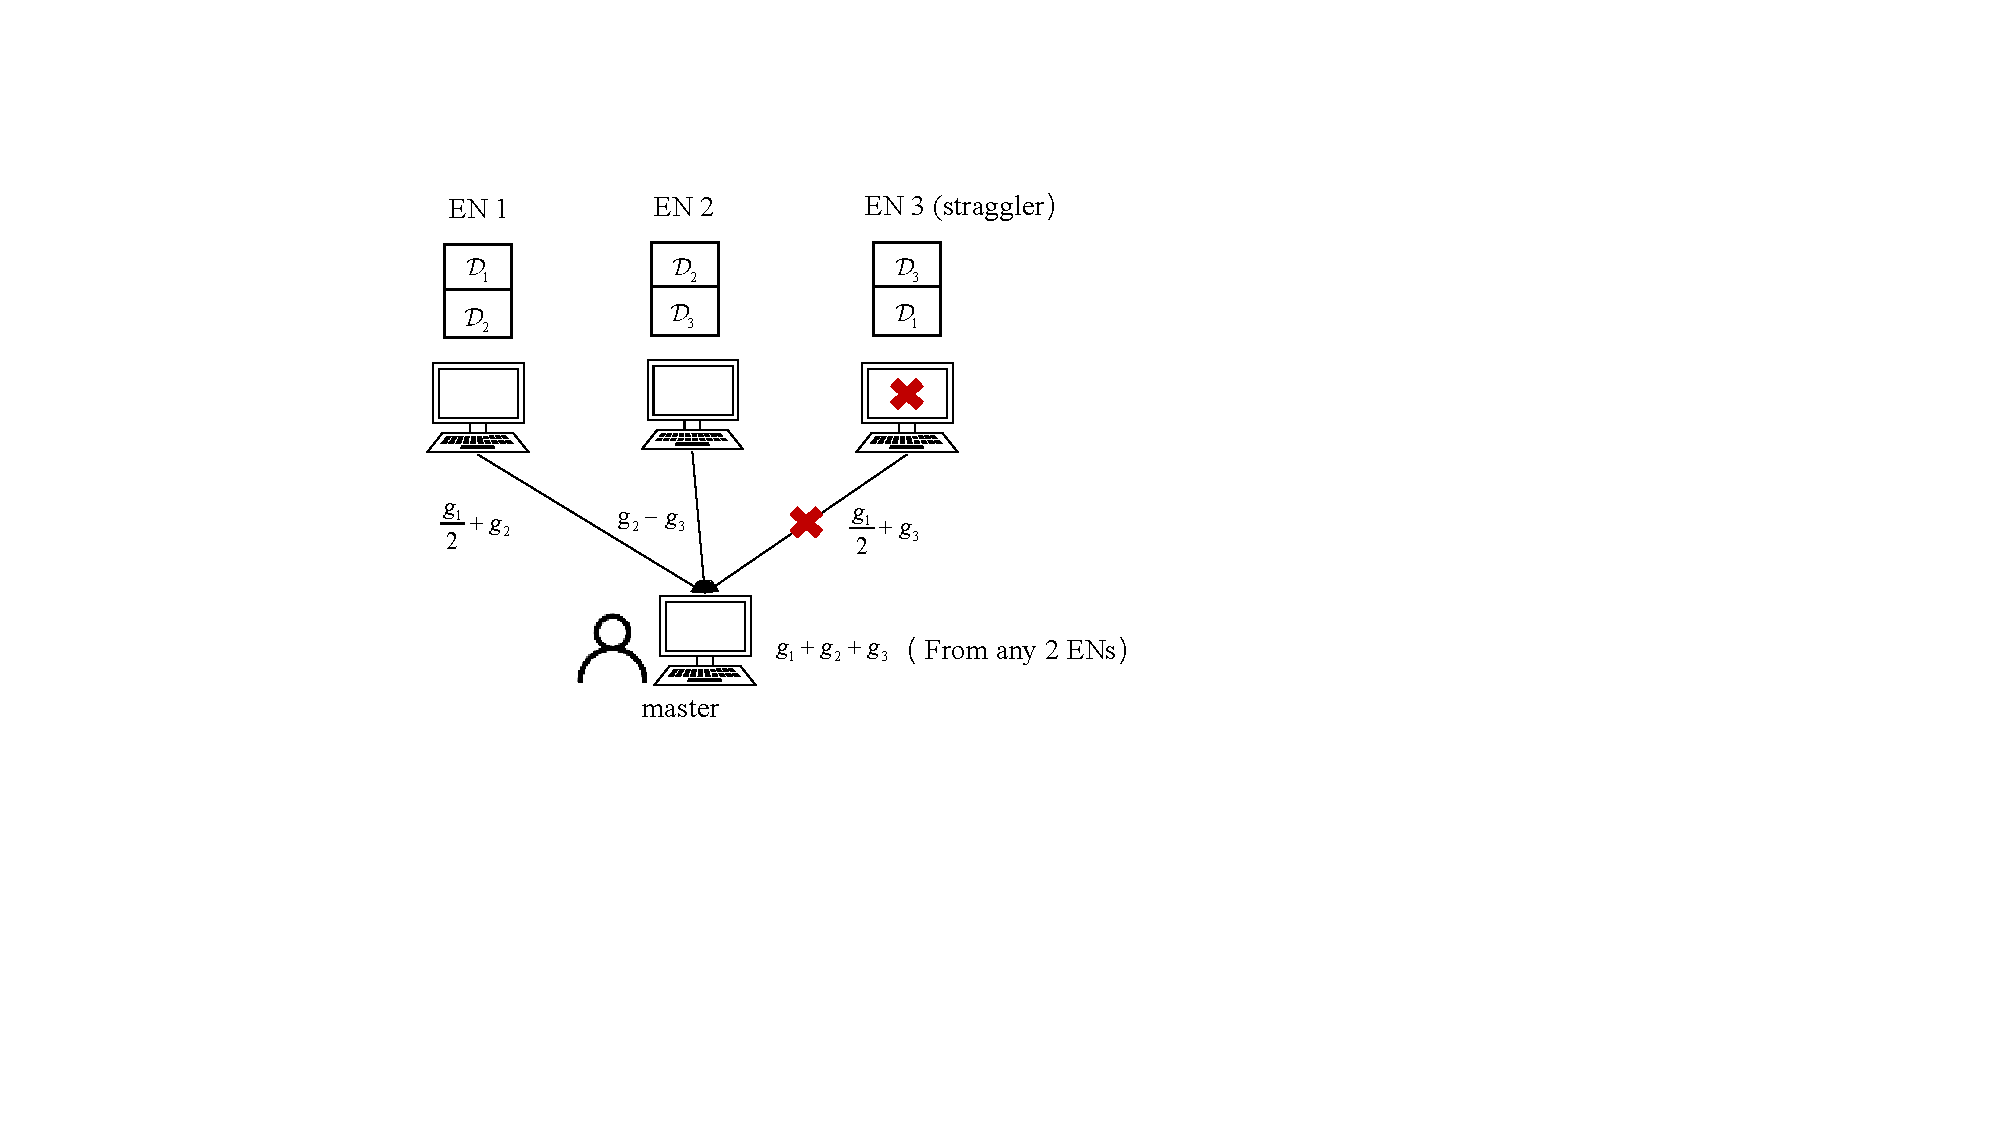
\includegraphics[width=0.5\textwidth]{gradient_coding.pdf}
	\caption{梯度编码计算}
	\label{gradient coding_chapter}
\end{figure}

\subsection{梯度编码计算模型}

%计算完成后，该梯度编码$\tilde{\mathbf{g}}_n^{(t)}$将被回传至移动设备，假设每个元素的梯度结果信息熵为$H(\tilde{g})$。

假设在计算完成时间内，移动设备仅接收到来自非迟滞节点集合$\mathcal{G}\subseteq[N]$的编码梯度$\left\{\tilde{\mathbf{g}}_{k}^{(t)}\right\}_{k\in\mathcal{G}}$。只要完成计算的节点数量满足$|\mathcal{G}|\geq N-S$，梯度编码方案即保证全梯度可恢复。具体来说，移动设备寻找一组解码系数向量$\mathbf{A}_{\mathcal{G}}=\{a_k\}_{k\in \mathcal{G}}$，使得该向量与完成计算的编码矩阵行向量的线性组合等于全$\mathbf{1}$向量，即求解以下线性方程组
\begin{align}
	\sum_{k\in\mathcal{G}}a_k\mathbf{b}_k=\mathbf{1}_{1\times K},
\end{align}
其中$\mathbf{b}_k$是矩阵$\mathbf{B}$的第$k$行，$\mathbf{1}_{1\times K}$是$K$维全1行向量。这确保了对于任意大小为$N-S$的子集，该方程均有解。
求解解码系数$\{\mathbf{a}_n\}_{n\in\mathcal{F}}$后，移动设备通过加权求和接收到的编码梯度来恢复全梯度值
\begin{align}
	\sum_{k\in\mathcal{G}}a_k\tilde{\mathbf{g}}_k^{(t)}=\sum_{k\in\mathcal{G}}a_k\left(\sum_{i=1}^Kb_{k,i}\mathbf{g}_i^{(t)}\right)=\sum_{i=1}^K\left(\sum_{k\in\mathcal{G}}a_kb_{k,i}\right)\mathbf{g}_i^{(t)}=\mathbf{1}\cdot \mathbf{g}_i^{(t)}=\mathbf{g}^{(t)}.
\end{align}
最后，移动设备利用重构的$\mathbf{g}^{(t)}$执行模型参数更新$w^{(t+1)}=w^{(t)}-\lambda \mathbf{g}^{(t)}$，其中$\lambda$表示迭代的步长。

\subsection{下行传输模型}

在计算完成后，从完成计算的节点$\mathcal{G}$中选取信道条件最好的$K$个节点进行传输，记为$\mathcal{K}=\{\pi(1),\cdots,\pi(K)\}$，假设这$K$个节点的信道条件满足$h_{\pi(1)}\geq h_{\pi(2)}\geq \cdots\geq h_{\pi(K)}$。为了提升频谱效率，和上一章节所提传输模型类似，本节也将采用功率域NOMA作为示例，采用其他的多址传输方案例如RSMA也适用。因此，这$K$个节点将被选取参与下行传输，第$k$个边缘节点的下行传输速率$R_k$可以表示为
\begin{equation}
	R_k=B_d\log_2\left(1+\frac{h_kp_k}{B_dn_0+\sum_{j=i+1}^{r}h_jp_j}\right)\label{sic_chapter_4},~\forall k\in\mathcal{K},
\end{equation}
其中$p_k$表示节点$k$的发射功率，$B_d$表示下行传输的带宽，$n_0$表示噪声功率。
类似地，在下行传输前，通常需要将计算结果进行信源编码，$K$个节点的信源编码速率$\tilde{R}_{c,i}$'s和传输速率$R_i$'s 需要满足
\begin{align}
	R_iT_d\geq\tilde{R}_{c,i} s,~\forall i\in\mathcal{K} \label{rt>l}
\end{align}
其中$T_d$表示下行传输延迟，$s$表示每个节点需要传输的梯度计算结果包含的符号数。

本研究旨在提升梯度编码场景中下行传输效率，降低传输时延。传统的传输方案往往会在传输之前对局部梯度值进行信源编码，一些工作采用直接编码方案，即只要信源编码速率满足
\begin{equation}
	\tilde{R}_{c,i}\geq H(\tilde{g}_i),~\forall i\in \mathcal{K}.
\end{equation}
然而，这种直接编码方案将边缘节点下行传输过程视为独立传输过程，并未有效利用节点间计算结果的相关性。由于梯度编码场景中，移动设备需要恢复局部梯度和，如果采用上一章所述的SW定理进行信源编码，本质上仍是恢复局部梯度$\tilde{\mathbf{g}}_k^{(t)}$（$k\in\mathcal{K}$）的值，再利用解码矩阵进行全梯度恢复。如果在信源编码阶段按照线性恢复的方案进行压缩，或许能进一步对局部梯度进行压缩，从而减少冗余信息的传输，提升传输效率。为此，本研究进一步提出了面向线性恢复的DSC辅助编码计算下行传输机制，通过嵌套线性码实现局部梯度值的分布式信源压缩，达到比独立恢复更大的压缩区域，从而提升编码效果。

\subsection{面向线性恢复的 DSC 辅助传输机制}\label{4.3}
本节将详细阐述所提面向线性恢复的DSC辅助编码计算结果下行传输机制，进一步建立下行传输时延优化问题。由于梯度编码场景中，每次迭代$t$移动设备仅需恢复梯度和$\mathbf{g}^{(t)}$。在选取的$K\in \mathcal{K}$个边缘节点传输局部梯度值之前，考虑采用基于嵌套线性码实现的信源编码方案\upcite{lim2019towards}。在无损且无边信息条件下，下面的定理给出了该方案能达到的信源编码速率区域。

\begin{theorem}\label{bcst}
	速率元组$(\tilde{R}_{c,1},\cdots,\tilde{R}_{c,K})$是可达的，只要它包含在以下区域$\mathcal{h}_{lossless}$中
	\begin{equation}
		\mathcal{h}_{lossless}=\bigcup_{\mathbf{E}}\bigcap_{\mathbf{C}}\bigcup_{\mathcal{S}}\bigcap_{\mathcal{T}}\left\{(\tilde{R}_{c,1},\cdots,\tilde{R}_{c,K})\in \mathbb{R}_+^K: \sum_{i\in\mathcal{T}}\tilde{R}_{c,i}>H(\hat{\mathbf{g}}_{\mathbf{E}}|\hat{\mathbf{g}}_{\mathbf{C}\mathbf{E}})\right\},\label{lossless_region}
	\end{equation}
	其中$\hat{\mathbf{g}}_{\mathbf{E}}^{(t)}=\mathbf{E}[\tilde{\mathbf{g}}_1,\cdots,\tilde{\mathbf{g}}_K]^T$，$\hat{\mathbf{Y}}_{\mathbf{C}\mathbf{E}}=\mathbf{C}\mathbf{E}[\tilde{\mathbf{g}}_1,\cdots,\tilde{\mathbf{g}}_K]^T$，集合运算是针对所有满足以下约束的元组（$\mathbf{E},\mathbf{C},\mathcal{S},\mathcal{T}$）进行的
	
	（a）$\mathbf{E}\in \mathbb{F}_q^{L_{\mathbf{E}\times K}}$遍历所有满秩矩阵，使得$1\leq L_{\mathbf{E}}\leq K$且span($\mathbf{E}$)$\supseteq$span($\tilde{\mathbf{F}}$)。
	
	（b）$\mathbf{C}\in \mathbb{F}_q^{L_{\mathbf{C}}\times L_{\mathbf{E}}}$遍历所有满秩矩阵（包括空矩阵），使得$0\leq L_{\mathbf{C}}< L_{\mathbf{E}}$。
	
	（c）$\mathcal{S}\subseteq[1:L_{\mathbf{E}}]$遍历所有大小为$|\mathcal{S}|=L_{\mathbf{E}}-L_{\mathbf{C}}$且满足
	\begin{equation}
		\textrm{rank}\left(\left[\begin{matrix}
			C\\
			\textbf{\textrm{I}}_{L_{\mathbf{E}}}(\mathcal{S})
		\end{matrix}\right]\right)=L_{\mathbf{E}},\label{rankc}
	\end{equation}
	
	（d）$\mathcal{T}\subset[K]$ 遍历所有大小为$|\mathcal{T}|=L_{\mathbf{E}}-L_{\mathbf{C}}$且满足
	\begin{equation}
		\textrm{rank}\left(\left[\begin{matrix}
			\mathbf{E}(\mathcal{S})\\
			\textbf{\textrm{I}}_K([K] \backslash \mathcal{T})
		\end{matrix}\right]\right)=K.\label{ranke}
	\end{equation}
	
\end{theorem}

%考虑文献\cite{lim2019towards}提出的基于代数网络信息论的嵌套信源编码方法，针对梯度编码场景中恢复结果是计算任务的线性组合，无损恢复且无边信息，完全恢复目标函数信源编码方法和经典SW定理不同，嵌套信源编码方法的可达区域为
%\begin{align}
%	\mathcal{h}_{comp}=\bigcup_{\mathbf{E}}\bigcap_{\mathbf{C}}\bigcup_{\mathcal{S}}\bigcap_{\mathcal{T}}\left\{(\eta_{\pi(1)},\cdots,\eta_{\pi(r)})\in \mathbb{R}_+^r: \sum_{i\in\mathcal{T}}\eta_i>H(\hat{\mathbf{Y}}_E|\hat{\mathbf{Y}}_{\mathbf{C}\mathbf{E}})\right\},\label{bcst}
%\end{align}
%其中，$\hat{\mathbf{Y}}_{\mathbf{E}}=\mathbf{E}[\mathbf{g}_{\pi(1)}^{(t)},\cdots,\mathbf{g}_{\pi(r)}^{(t)}]^T, \hat{\mathbf{Y}}_{\mathbf{C}\mathbf{E}}=\mathbf{C}\mathbf{E}[\mathbf{g}_{\pi(1)}^{(t)},\cdots,\mathbf{g}_{\pi(r)}^{(t)}]^T$，且所有元组（$\mathbf{E},\mathbf{C},\mathbf{\mathcal{S}},\mathbf{\mathcal{T}}$）满足定理\ref{<theorem-chapter-4>}中的(b)-(d)以及
%
%（a）$\mathbf{E}\in \mathbb{F}_q^{L_{\mathbf{E}\times r}}$遍历所有满秩矩阵，使得$1\leq L_{\mathbf{E}}\leq r$且span($\mathbf{E}$)$\supseteq$span($\mathbf{F}$)。
%
%因此，在节点完成计算结果后，采用文献\cite{lim2019towards}中的信源编码方案进行信源压缩，可以实现(\ref{bcst})达到的信源压缩区域。

\begin{remark}
定理\ref{bcst}是定理\ref{<theorem-chapter-2>}应用在梯度编码场景中的简化形式，即不考虑边信息且能够无损恢复信源。
\end{remark}

% \subsection{任务总执行时延推导}

\subsection{最小化下行传输时延优化问题}

基于嵌套线性码（具体编码方案详见附录\ref{<nested linear coding>}）构成的信源压缩区域，边缘节点可以根据信道条件调整其压缩率。相应的优化问题可以建模如下
\begin{align}
	\mathcal{P}_{4.1}:& \min_{\mathbf{R},\mathbf{p}, \tilde{\mathbf{R}}_{c},T_d} ~T_{d}\\
	\text{s.t.}~ &(\ref{sic_chapter_4}),(\ref{rt>l}),(\ref{lossless_region}),(\ref{rankc}),(\ref{ranke})\notag,\\
	& 0\leq p_i\leq P_{max}, \label{pmax}~\forall i\in \mathcal{G},
\end{align}
其中 $\mathbf{R} = [R_{\pi(1)}, R_{\pi(2)}, \cdots, R_{\pi(K)}]$, $\mathbf{p} = [p_{\pi(1)}, p_{\pi(2)}, \cdots, p_{\pi(K)}]$, 以及 $\tilde{\mathbf{R}}_{c}=[\tilde{R}_{c,1},\cdots,\tilde{R}_{c,K}]$ 是相应变量的紧凑表示；$P_{max}$ 是每个 节点的最大发射功率；

\begin{remark}
	相比于经典Slepian-Wolf定理的信源可达区域，在梯度编码场景中，移动设备不用恢复完整子任务的计算结果，再将计算结果进行求和，而只需要恢复线性组合。利用嵌套线性码可以达到各节点信源压缩时按照线性特定关系进行编码压缩，从而达到比恢复各节点计算结果更大的压缩区域，因此扩大了优化区域。
\end{remark}

\section{面向线性恢复的DSC辅助编码计算结果传输算法}\label{4.4}
由于问题$P_{4.1}$直接利用区域$\mathcal{h}_{lossless}$进行优化，需要遍历满足（a）-（d）所有的情况，增加优化问题的复杂度，为了保证优化的区域以及优化问题求解的复杂度不会过高，可以利用边界条件进行简化。
\begin{theorem}\label{<linear>}
	针对面向线性恢复的计算结果下行传输场景，基于嵌套线性码的低复杂度可达速率区域$\mathcal
	h_{sub}$定义为独立数据恢复边界$\mathcal{h}_{sw}$与线性直接恢复边界$\mathcal{h}_{linear}$的并集
	\begin{equation}
		\mathcal{h}_{sub} \triangleq \mathcal{h}_{sw} \cup \mathcal{h}_{linear},
	\end{equation}
	其中，
	\begin{align}
		&\mathcal{h}_{sw}=\left\{(\tilde{R}_{c,k}):\sum_{k\in\mathcal{L}}\tilde{R}_{c,k}>H\left(\{\mathbf{\tilde{g}}_k\}_{k\in\mathcal{L}}|\{\mathbf{\tilde{g}}_n\}_{n \notin\mathcal{L}}\right), \forall \mathcal{L}\subseteq \mathcal{K}\right\},\label{hsw}\\
		&\mathcal{h}_{linear}=\left\{(\tilde{R}_{c,k}): \tilde{R}_{c,k}>H\left(\mathbf{g}^{(t)}\right),\forall k\in \mathcal{K}\right\}.\label{hlinear}
	\end{align}
	任何落在该并集区域内的速率元组均可实现全梯度$\mathbf{g}^{(t)}$的无损重构。
\end{theorem}
\begin{proof}
	推导见附录\ref{<linear-proof>}。
\end{proof}

因此，问题$P_{4.1}$可以近似简化为
\begin{align}
		\mathcal{P}_{4.2}:& \min_{\mathbf{R},\mathbf{p}, \tilde{\mathbf{R}}_{c},T_d} ~T_{d}\\
	\text{s.t}.~ &(\ref{sic_chapter_4}),(\ref{rt>l}),(\ref{pmax}),(\ref{hsw}), (\ref{hlinear})\notag.
\end{align}
更进一步，可以将信源压缩区域拆分成两个子区域分别进行优化，即问题$P_{4.2}$可以等价的分为$P_{4.3}$和$P_{4.4}$的最小值，即$P_{4.2}=\min \left\{P_{4.3},P_{4.4}\right\}$，其中$P_{4.3}$和$P_{4.4}$可以分别表示为
\begin{align}
	\mathcal{P}_{4.3}:& \min_{\mathbf{R},\mathbf{p}, \tilde{\mathbf{R}}_{c},T_d} ~T_{d}\\
	\text{s.t}.~ &(\ref{sic_chapter_4}),(\ref{rt>l}),(\ref{pmax}),(\ref{hsw})\notag.
\end{align}
以及
\begin{align}
	\mathcal{P}_{4.4}:& \min_{\mathbf{R},\mathbf{p}, \tilde{\mathbf{R}}_{c},T_d} ~T_{d}\\
	\text{s.t}.~ &(\ref{sic_chapter_4}),(\ref{rt>l}),(\ref{pmax}), (\ref{hlinear})\notag.
\end{align}

类似地，由于子问题$P_{4.3}$和子问题$P_{4.4}$都是非凸问题，与第三章算法类似，可以通过转换为凸差问题，使用CCCP技术求解。具体来说，公式（\ref{sic_chapter_4}）以及公式（\ref{rt>l}）同样可以通过引入辅助变量$\{\mu_i\}_{i=1}^K$以及$\{\nu_i\}_{i=1}^K$，等价转为DC形式
\begin{subnumcases}
	{}\nu_i=\frac{1}{2}\left(R_i+T_d\right),~\forall i\in\mathcal{K},\label{zc}\\
	\mu_i=\frac{1}{2}(R_i-T_d),~\forall i\in\mathcal{K},\label{xc}\\
	\nu_i^2-\mu_i^2- \tilde{R}_{c,i}s\geq 0,~\forall i\in\mathcal{K}.\label{zxc}
\end{subnumcases}
公式(\ref{sic_chapter_4})已经是一个DC形式的约束，因此问题$\mathcal{P}_{4.3}$和$\mathcal{P}_{4.4}$可以等价转化为
\begin{align}
	\mathcal{P}_{4.5}:& \min_{\mathbf{R},\mathbf{p}, \tilde{\mathbf{R}}_{c},T_d} ~T_{d}\\
	\text{s.t}.~ &(\ref{sic_chapter_4}),(\ref{pmax}),(\ref{hsw}),(\ref{zc}),(\ref{xc}),(\ref{zxc})\notag.
\end{align}
以及
\begin{align}
	\mathcal{P}_{4.6}:& \min_{\mathbf{R},\mathbf{p}, \tilde{\mathbf{R}}_{c},T_d} ~T_{d}\\
	\text{s.t}.~ &(\ref{sic_chapter_4}),(\ref{pmax}), (\ref{hlinear}),(\ref{zc}),(\ref{xc}),(\ref{zxc})\notag.
\end{align}
求解$\mathcal{P}_{4.5}$和$\mathcal{P}_{4.6}$可以利用CCCP算法。在第$(\tau+1)$次迭代中，利用第$\tau$次迭代得到的最优解（$\mathbf{R}^{(\tau)},\mathbf{p}^{(\tau)},\symbfit{\nu}^{(\tau)},\symbfit{\mu}^{(\tau)},\tilde{\mathbf{R}}_{c}^{(\tau)}$），对约束中的凹部分进行线性化近似求解，其中$\mathbf{R}^{(\tau)}=[R_1^{(\tau)},\cdots,R_{K}^{(\tau)}],\mathbf{p}^{(\tau)}=[p_1^{(\tau)},\cdots,p_{K}^{(\tau)}],\symbfit{\mu}^{(\tau)}=[\mu_1^{(\tau)},\cdots,\mu_{K}^{(\tau)}],\symbfit{\nu}^{(\tau)}=[\nu_1^{(\tau)},\cdots,\nu_{K}^{(\tau)}],$$\mathbf{R}_{c}^{(\tau)}=[R_{c,1}^{(\tau)},\cdots,R_{c,K}^{(\tau)}]$为优化变量的向量形式。具体而言，第（$\tau$+1）次迭代中（\ref{zxc}）可以近似为
\begin{equation}
		\mu_i^2-\left(\left({\nu_i}^{(\tau)}\right)^2+2\nu_i^{(\tau)}\left(\nu_i-\nu_i^{(\tau)}\right)\right)
	+ \tilde{R}_{c,i}s\leq 0,~ \forall i\in\mathcal{K}.\label{cccp3}
\end{equation}
类似的，（\ref{sic_chapter_4}）的凹部分可以参考第三章（\ref{cccp2}）进行线性化
	\begin{align}
	R_i\geq &
	B_d\log_2\left({B_dn_0+\sum\nolimits_{j={i}}^{K}h_jp_j}\right)
	-B_d\log_2\left({B_dn_0+\sum\nolimits_{j={i+1}}^{K}h_jp_j^{(\tau)}}\right)\notag\\&-
	B_d\left(\frac{\sum_{j={i+1}}^{K}h_j\left(p_{j}-p_{j}^{(\tau)}\right)}{(\ln2)\left(\sum_{j={i+1}}^{K}h_jp_{j}^{(\tau)}+Bn_0\right)}\right),~\forall i\in\mathcal{K}\label{cccp4}.
\end{align}
因此，在第$(\tau+1)$次迭代中，$\mathcal{P}_{4.5}$和$\mathcal{P}_{4.6}$可以近似转化为如下凸问题
\begin{align}
	\mathcal{P}_{4.7}:& \min_{\mathbf{R},\mathbf{p}, \tilde{\mathbf{R}}_{c},T_d} ~T_{d}\\
	\text{s.t}.~ &(\ref{pmax}),(\ref{hsw}),(\ref{zc}),(\ref{xc}),(\ref{cccp3}),(\ref{cccp4})\notag.
\end{align}
以及
\begin{align}
	\mathcal{P}_{4.8}:& \min_{\mathbf{R},\mathbf{p}, \tilde{\mathbf{R}}_{c},T_d} ~T_{d}\\
	\text{s.t}.~ &(\ref{pmax}), (\ref{hlinear}),(\ref{zc}),(\ref{xc}),(\ref{cccp3}),(\ref{cccp4})\notag.
\end{align}
$\mathcal{P}_{4.7}$和$\mathcal{P}_{4.8}$可以通过标准方法求解，具体过程见算法1。

\begin{algorithm}[h]
	%				\footnotesize
	\caption{面向线性恢复的DSC辅助编码计算结果下行传输算法}
	%			\begin{algorithmic}[1]
%		\SetKwInOut{Input}{输入}\SetKwInOut{Output}{输出}
		\SetKwRepeat{Repeat}{repeat}{until}%
		\LinesNumbered
%		\Input{容差 $\epsilon$, 功率约束 $P_{max}$,任务包大小 $l$;}
%		\Output{传输速率 $\mathbf{R}^*$, 发射功率 $\mathbf{p}^*$, 信源压缩率 $\symbfit{\eta}^*$, 下行传输延迟 $T_d^*$;}
		初始化：算法收敛精准度$\epsilon$，发射功率约束$P_{max}$，传输包符号数$s$;\\
		选择一个初始可行点 ($\mathbf{p}_{sw}^{(0)}$, $\symbfit{\nu}_{sw}^{(0)}$) ，并设置迭代次数 $\tau=1$;\\
		\Repeat{$|T_{d_{sw}}^{(\tau)}-T_{d_{sw}}^{(\tau-1)}|\leq \epsilon$}{
			基于 $\left\{\left(\mathbf{R}_{sw}^{(\tau)},\mathbf{p}_{sw}^{(\tau)},\symbfit{\nu}_{sw}^{(\tau)},\symbfit{\mu}_{sw}^{(\tau)},\symbfit{\bar{\eta}}_{sw}^{(\tau)}\right)\right\}$求解 $\mathcal{P}_{4.7}$ ;\\
			计算 $T_{d_{sw}}^{(\tau+1)}$;\\
			令 $\tau=\tau+1$;}
		\Repeat{$|T_{d_{linear}}^{(\tau)}-T_{d_{linear}}^{(\tau-1)}|\leq \epsilon$}{
			 基于 $\left\{\left(\mathbf{R}_{linear}^{(\tau)},\mathbf{p}_{linear}^{(\tau)},\symbfit{\nu}_{linear}^{(\tau)},\symbfit{\mu}_{linear}^{(\tau)},\symbfit{\bar{\eta}}_{linear}^{(\tau)}\right)\right\}$求解 $\mathcal{P}_{4.8}$;\\
			计算 $T_{d_{linear}}^{(\tau+1)}$;\\
			令 $\tau=\tau+1$;}
			\If{$T_{d_{linear}}<T_{d_{sw}}$}
			{\text{返回}\quad$\mathbf{R}^*=\mathbf{R}_{linear}^{(\tau)}$, $\mathbf{p}^*=\mathbf{p}_{linear}^{(\tau)}$, $\symbfit{\eta}^*=\symbfit{\eta}_{linear}^{(\tau)}$, $T_d^*=T_{d_{linear}}^{(\tau)}$.}
		\Else
		{\text{返回}\quad$\mathbf{R}^*=\mathbf{R}_{sw}^{(\tau)}$, $\mathbf{p}^*=\mathbf{p}_{sw}^{(\tau)}$, $\symbfit{\eta}^*=\symbfit{\eta}_{sw}^{(\tau)}$, $T_d^*=T_{d_{sw}}^{(\tau)}$.}
		
		%			\end{algorithmic}	
\end{algorithm}

\begin{corollary}\label{condition}
	考虑特殊情况，即所有完成计算节点的下行传输信道条件相同时，当且仅当全梯度的熵$H(\mathbf{g}^{(t)})$与局部编码梯度的联合熵$H(\left\{\tilde{\mathbf
	{g}}_k\right\}_{k\in\mathcal{K}})$满足以下条件时，采用线性直接恢复压缩策略$\mathcal{h}_{linear}$比经典Slepian-Wolf策略$\mathcal{h}_{sw}$具有更低的传输延迟
	\begin{align}
		H(\left\{\tilde{\mathbf{g}}_k\right\}_{k\in\mathcal{G}})>r \cdot H(\mathbf{g}^{(t)}).
	\end{align}
	直观理解，该条件意味着梯度编码引入的数据冗余度与局部噪声之比超过了完成计算节点的数量。
\end{corollary}
\begin{proof}
	证明详见证明\ref{<condition>}。
\end{proof}


\section{仿真性能与分析}\label{4.5}
本节将通过数值仿真验证所提机制的有效性。
在仿真中，对于下行传输，采用瑞利衰落信道模型 $h_i = |\mathbf{h}_i|^2 \rho$ \cite{goldsmith2005wireless}，其中 $\rho$ 为平均增益，小尺度衰落系数 $\mathbf{h}_i$ 服从复高斯分布 $\mathcal{CN}(0, 1)$。
噪声功率谱密度 $n_0$ 设定为 $1 \times 10^{-17}$ (W/Hz)，下行信道带宽 $B$ 设定为 20 (MHz)。
此外，由于嵌套线性码的性能与我们的工作是正交的，假设采用理想的嵌套线性码实现无损恢复。完成计算并参与下行传输的 $K$ 个 边缘节点是随机选择的，并基于这些选择的 节点执行 $1 \times 10^4$ 次蒙特卡洛运行以获得平均性能。梯度编码中，考虑采用循环重复编码方案，分别考虑两种场景：一是边缘节点数目与子任务划分数目相等，均为$N=5$，恢复阈值为$K=3$，二是边缘节点数目与子任务划分数目相等，均为$N=7$，恢复阈值为$K=4$。
为了验证所提机制的有效性，本节通过仿真实验对比了以下两种基线方案的性能：
 基线方案一考虑传统信源独立编码方式，即各边缘节点独立传输计算结果，不进行分布式信源编码压缩。基线方案二考虑采用理论 SW编码对各边缘节点进行分布式信源压缩，利用 SW 理论区域进行完整数据恢复的压缩传输方案。



\begin{figure}[htbp]
    \centering
    \includegraphics[width = 0.75 \textwidth]{figs/real_channel_gain_Chinese.eps}
    \caption{不同平均信道增益$\rho$下的下行传输时延$T_d$比较（最大发射功率约束$P_{max}=0.2$（W））。}
    \label{fig:4.2}
\end{figure}

图~\ref{fig:4.2}展示了在不同平均信道功率增益$\rho$下，分别对参数$N=5$和$K=3$以及$N=7$和$K=4$对平均下行传输时延$T_d$的性能比较。可以观察到，利用理论SW编码方案和所提基于线性码的线性恢复编码方案相比于基线方案一都有明显的性能提升。例如，当平均信道增益为$\rho=-115$（dB）且参数$N=5,K=3$的场景下，所提面向线性恢复传输方案的下行平均传输延迟为$0.078$（ms），基线方案二面向独立恢复传输方案的下行平均传输延迟为$0.084$（ms），都比基线方案一独立传输方案的下行平均延迟$0.097$（ms）低，且所提方案相比于基线方案二也降低了传输延迟，这是由于所提方案在面向计算结果线性恢复的场景中，利用嵌套线性码能够达到更大的信源编码区域，从而达到更好的负载重分配的效果。当平均信道增益为$\rho=-115$（dB）且参数$N=7,K=4$的场景下，所提面向线性恢复传输方案相比于基线方案一的性能增益为$49\%$，相比于基线方案二的性能增益为$6\%$。可以看出，当节点数增加后，相比于基线方案一，所提方案有了更明显的性能提升。这是因为，当节点数增加后，信道条件差的节点出现的概率增大。基线方案一中每个节点独立传输，如果其中一个节点的信道条件较差，会影响整体的传输延迟。而所提方案采用了面向线性恢复的DSC方案，可以实现节点间传输负载的重分配效果，使得信道条件差的节点少传一部分信息，信道条件好的节点多传一部分信息，从而避免了单个节点影响整体传输性能。


\begin{figure}[htbp]
	\centering
	\includegraphics[width = 0.75 \textwidth]{figs/real_transmit_power_Chinese.eps}
	\caption{不同最大发射功率$P_{max}$下的下行传输时延$T_d$比较（平均信道增益为$\rho=-110$（dB）。}
	\label{fig:4.3}
\end{figure}
图~\ref{fig:4.3}展示了在不同最大发射功率$P_{max}$下，分别对参数$N=5$和$K=3$以及$N=7$和$K=4$对平均下行传输时延$T_d$的性能比较。可以观察到，所提方案相比于基线方案仍然有显著的性能增益。例如，当$P_{max}=0.05$（W）且参数$N=5,K=3$的场景下，所提方案相比于基线方案一的性能增益为$50\%$，相比于基线方案二的性能增益为$8\%$。当$P_{max}=0.05$（W）且参数$N=7,K=4$的场景下，所提方案相比于基线方案一的性能增益为$58\%$，相比于基线方案二的性能增益为$14\%$。此外，当最大发射功率越小时，性能增益越明显。例如，当$P_{max}=0.45$（W）且参数$N=5,K=3$的场景下，所提方案相比于基线方案一的性能增益为$42\%$，当参数$N=7,K=4$的场景下，所提方案相比于基线方案一的性能增益为$37\%$。进一步验证了，当信道条件差的情况下，所提方案能够提供更灵活的信源编码区域，达到负载重分配的效果。


%图~\ref{fig:4.2} 和图~\ref{fig:4.4} 展示了在不同平均信道功率增益 $\rho$ 下，平均任务执行时延 $T_d$ 的性能比较。其中图例分别展示了两种不同的系统配置：配置一为 $r=3, k=5$（实心点曲线），配置二为 $r=4, k=7$（空心点曲线）。可以观察到，随着信道条件 $\rho$ 的改善（从 $-115\text{ dB}$ 增加到 $-105\text{ dB}$），所有方案的时延均显著降低。然而，在相同的信道条件下，本文提出的基于代数嵌套线性码的方案始终优于基准方案和基于理想 SW 码的方案。例如，在 $\rho = -115\text{ dB}$ 且 $r=3, k=5$ 的情况下，基准方案的时延约为 $160\text{ ms}$，理想 SW 方案的时延约为 $125\text{ ms}$，而采用代数嵌套线性码的方案时延仅为 $105\text{ ms}$ 左右。这证实了定理 4.3 的结论，即针对梯度聚合等线性计算任务，直接恢复函数值的压缩效率要高于恢复完整原始数据，从而能获得更大的可达速率区域和更低的传输时延。此外，相比于独立传输的基准方案，所提方案利用了重复计算引入的冗余信息进行协作传输，有效缓解了深衰落节点对系统性能的限制。
\begin{figure}[htbp]
	\centering
	\includegraphics[width = 0.75 \textwidth]{figs/equal_channel_gain_Chinese.eps}
	\caption{边缘节点信道条件相同，不同平均信道增益$\rho$下的下行传输时延$T_d$比较（最大发射功率约束$P_{max}=0.2$（W））。}
	\label{fig:4.4}
\end{figure}
图~\ref{fig:4.4}展示了边缘节点平均信道功率增益相同的情况下，平均下行传输时延$T_d$的性能比较。类似地可以观察到，当信道条件越差时，所提方案相较于基线方案一的性能增益越明显。例如，当参数$N=5,K=3$的场景下，$\rho=-105$（dB）时，所提方案对比基线方案一的性能增益为$29\%$，当$\rho=-115$（dB）时，所提方案对比基线方案的性能增益为$30\%$。当参数$N=7,K=4$的场景下，$\rho=-105$（dB）时，所提方案对比基线方案一的性能增益为$37\%$，当$\rho=-115$（dB）时，所提方案对比基线方案的性能增益为$38\%$。
在信道条件相同的情况下，随着信道条件越差 所提方案相比于基线方案二的性能增益也有所提升。例如，当参数$N=5,K=3$的场景下，$\rho=-105$（dB）时，所提方案相比于基线方案二的性能增益为$8\%$，当$\rho=-115$（dB）时，所提方案相比于基线方案二的性能增益为$11\%$。这是由于所提方案的DSC可行域比基线方案二的DSC区域多出来一个拐点，即与推论\ref{condition}所给出的内容一致，验证了所提方案相比基线方案二的性能优势。

图~\ref{fig:4.5}展示了边缘节点平均信道功率相同的情况下（$\rho=-110$（dB）），比较不同最大发射功率$P_{max}$条件下的下行传输时延$T_d$。类似地可以观察到当$P_{max}=0.05$（W）时，所提方案相比于基线方案一的性能增益在$N=5,K=3$和$N=7,K=4$场景下分别为$26\%$和$24\%$。所提方案相比于基线方案二的性能增益在$N=5,K=3$和$N=7,K=4$场景下分别为$7\%$和$8\%$。
\begin{figure}[htbp]
	\centering
	\includegraphics[width = 0.65 \textwidth]{figs/equal_transmit_power_Chinese.eps}
	\caption{边缘节点信道条件相同，不同最大发射功率$P_{max}$下的下行传输时延$T_d$比较（平均信道增益为$\rho=-110$（dB）。}
	\label{fig:4.5}
\end{figure}



%图~\ref{fig:4.3} 和图~\ref{fig:4.5} 展示了边缘节点最大传输功率 $P_{\max}$ 对平均任务执行时延的影响。从图中可以看出，随着发射功率预算的增加，下行传输速率提升，从而降低了总时延。在低功率区域（如 $P_{\max}=0.05\text{ W}$），所提方案的优势尤为明显。对比图中 $r=3, k=5$ 的情况，当 $P_{\max}=0.05\text{ W}$ 时，基于代数嵌套线性码的方案相较于基准方案降低了约 50\% 以上的时延。这是因为在功率受限的情况下，通信资源更为稀缺，本文提出的方案通过更高效的信源压缩（嵌套线性码）和功率分配优化，能够在有限的功率预算下实现更快速的结果汇聚。同时，图中的放大子图进一步清晰地展示了在高功率区域，虽然各方案间差距缩小，但所提方案依然保持了最低的时延性能，证明了其在不同信噪比环境下的鲁棒性。
%
%
%
%综合图~\ref{fig:4.2} 至图~\ref{fig:4.5} 的结果，可以得出结论：在分布式边缘计算的梯度聚合场景中，利用计算结果间的代数结构相关性，采用面向线性恢复的分布式信源编码策略，能够突破传统 Slepian-Wolf 编码的性能瓶颈，显著降低下行协作传输的时延。


\section{本章小结}\label{chapter-sum}
本章针对编码计算中计算结果下行传输过程由于可能存在信道深衰落造成的通信瓶颈问题，提出了一种面向线性恢复的DSC辅助下行传输机制。与现有将下行传输视为独立多用户通信的研究不同，本研究综合考虑了任务编码引入的计算冗余与通信阶段的协作传输增益之间的权衡。
针对梯度下降等线性聚合类任务，不再局限于恢复单个子任务的计算结果，而是利用嵌套线性码，构建了面向线性函数恢复的传输模型。理论分析表明，相比于经典的 SW定理完整重构信源，面向线性恢复的编码策略拥有更大的可达压缩区域。在此基础上，建立了以最小化任务总执行时延为目标的优化问题，并利用交替优化和差分凸规划算法联合优化了任务划分与下行传输功率分配。
仿真结果表明，所提出的基于代数嵌套线性码的DSC辅助下行传输方案在时延性能上显著优于传统的独立传输方案以及基于 SW定理 的完整恢复方案，特别是在信道条件较差或功率受限的场景下，能够有效降低系统的下行传输时延，提升编码计算整体处理任务的效率。
\chapter{总结与展望}

\section{全文总结}

编码边缘计算通过引入冗余缓解了分布式计算中的迟滞效应，但现有研究大多忽略了下行传输阶段由于信道衰落可能导致的通信时延问题。事实上，编码计算在任务分发阶段引入的冗余使得各边缘节点的计算结果之间存在强相关性，这为利用DSC技术优化下行传输提供了可能。本文从DSC的视角出发，研究了面向完整恢复和线性恢复两种场景下的编码计算结果传输方案，主要工作和贡献总结如下：

\begin{enumerate}
	\item[（1）]面向完整恢复的DSC辅助编码计算结果传输方法研究。针对需要完整恢复各子任务计算结果的场景，提出了基于LDPC码伴随式穿刺的DSC方案。该方案利用编码计算结果间的线性相关性，使边缘节点能够根据信道状态自适应调整压缩率，实现传输负载在节点间的灵活重分配。此外，将该方案扩展至高维数据场景，利用逐级编码思想处理多维度数据的压缩与传输。建立了下行传输时延最小化优化模型，设计了基于CCCP的联合优化算法。仿真结果表明，所提方案在信道条件异构场景下显著降低了传输时延，且对迟滞节点数量变化具有良好的鲁棒性。

	\item[（2）]面向线性恢复的DSC辅助编码计算结果传输方法研究。针对仅需恢复计算结果线性函数值的场景，提出了基于嵌套线性码的编码方案。证明了面向线性恢复的编码方案能够获得比经典SW编码更大的可达速率区域，从而实现更高的压缩效率。给出了可达速率区域的简化形式，降低了优化问题的求解复杂度。建立了相应的时延最小化优化模型，设计了联合优化算法。仿真结果验证了所提方案的下行传输性能均优于独立编码方案和SW编码方案，且随着迟滞节点数量增加，所提方案相比SW编码方案的优势更为明显。
\end{enumerate}


\section{未来展望}

本文针对编码计算中可能由于信道衰落导致的通信时延展开了研究，提出了面向完整恢复和面向线性恢复的DSC辅助编码计算结果下行传输方案。虽然提出的方案取得了一定的性能增益，但仍然存在一些问题有待进一步探索。
具体而言，未来可能的探索方向包括：

\begin{enumerate} [ label = （\arabic*）]
    \item 向具有更多边缘节点的密集边缘网络场景扩展。本文在仿真实验中验证了所提方案在中等规模边缘网络中的有效性，然而随着边缘计算技术的发展，未来边缘网络将呈现高密度部署态势。在密集边缘网络场景下，参与计算的边缘节点数量显著增加，这将为所提方案带来新的挑战。首先，大规模节点场景下优化问题的求解复杂度将显著上升，需要设计低复杂度的分布式或启发式求解算法。其次，节点数量的增加意味着更强的用户间干扰，需要研究更先进的多址接入技术或干扰管理策略。

    \item 设计具有更大信源编码可行域的编码方案。本文第三章提出的基于伴随式穿刺的DSC方案仅实现了理想SW区域的一个子区域，如何设计更逼近SW理论极限的实用化编码方案是一个值得探索的方向。一方面，可以研究基于极化码或空间耦合LDPC码的DSC方案，这类码字在有限码长下具有更好的性能逼近特性。另一方面，第四章提出的嵌套线性码方案虽然在特定条件下能够获得比SW区域更大的可达速率区域，但如何扩大该优势的适用条件范围仍有待研究。此外，可以探索机器学习辅助的信源编码方案，利用神经网络学习信源间的相关性结构，实现自适应的压缩编码设计。

    \item 上下行传输链路和计算阶段的联合优化。本文主要聚焦于编码计算的下行结果回传阶段，将上行任务分发和计算阶段视为已知条件。然而，在实际系统中，上行传输、边缘计算和下行传输三个阶段相互耦合、相互影响，联合优化有望进一步提升系统整体性能。具体而言，上行阶段的任务编码方案与下行阶段的信源压缩效率密切相关，不同的编码策略会导致计算结果间相关性的差异，进而影响DSC的压缩增益。此外，计算阶段的资源分配（如CPU频率调度）与通信阶段的功率控制存在耦合关系，需要建立跨计算与通信的联合资源优化框架。因此，研究涵盖上行-计算-下行全链路的联合优化机制具有重要的理论价值和应用前景。
\end{enumerate}

% \include{pages/chapter6}

\end{document}